%% 
%% Copyright 2019-2024 Elsevier Ltd
%% 
%% Version 2.4
%% 
%% This file is part of the 'CAS Bundle'.
%% --------------------------------------
%% 
%% It may be distributed under the conditions of the LaTeX Project Public
%% License, either version 1.2 of this license or (at your option) any
%% later version.  The latest version of this license is in
%%    http://www.latex-project.org/lppl.txt
%% and version 1.2 or later is part of all distributions of LaTeX
%% version 1999/12/01 or later.
%% 
%% The list of all files belonging to the 'CAS Bundle' is
%% given in the file `manifest.txt'.
%% 
%% Template article for cas-sc documentclass for 
%% single column output.

% \documentclass[a4paper,fleqn,longmktitle]{cas-sc}
\documentclass[a4paper]{cas-sc}
\usepackage[utf8]{inputenc}
\usepackage[numbers]{natbib} % allow utf-8 input
% \usepackage[margin=1in]{geometry}
\usepackage{indentfirst}
\usepackage[T1]{fontenc}    % use 8-bit T1 fonts
\usepackage{hyperref}      % hyperlinks
\usepackage[none]{hyphenat}
\usepackage{tikz}
\usetikzlibrary{quantikz2}
\usepackage{listings}
\usepackage{url}            % simple URL typesetting
\usepackage{booktabs}       % professional-quality tables
\usepackage{amsfonts}       % blackboard math symbols
\usepackage{nicefrac}       % compact symbols for 1/2, etc.
\usepackage{microtype}      % microtypography
\usepackage{lipsum}		% Can be removed after putting your text content
\usepackage{graphicx}
\usepackage{doi}
\usepackage{framed,multirow}
%% The amssymb package provides various useful mathematical symbols
\usepackage{amssymb}
\usepackage{latexsym}
\usepackage{graphicx}
\usepackage{amsmath}
\usepackage{booktabs} % for better looking tables
\usepackage{tabularx}
\usepackage{array}
\usepackage{etoolbox}
\usepackage{subcaption}
\usepackage{algorithm}
\usepackage{algorithmic}
\usepackage{indentfirst}
\usepackage{float}
\usepackage{arydshln}
\usepackage{svg}
\usepackage[nameinlink, noabbrev]{cleveref}
%%%Author macros
\def\tsc#1{\csdef{#1}{\textsc{\lowercase{#1}}\xspace}}
\tsc{WGM}
\tsc{QE}
\tsc{EP}
\tsc{PMS}
\tsc{BEC}
\tsc{DE}
%%%

\begin{document}
\let\WriteBookmarks\relax
\def\floatpagepagefraction{1}
\def\textpagefraction{.001}
\shorttitle{Quantum-assisted Secure Audio Communication}
\shortauthors{Md. Raisul Islam Rifat et~al.}
%\begin{frontmatter}

\title [mode = title]{QSAC: Quantum-assisted Secure Audio Communication using Quantum Entanglement, Audio Steganography, and Classical Encryption}


% \tnotetext[1]{This document is the results of the research
%     project funded by the National Science Foundation.}

% \tnotetext[2]{The second title footnote which is a longer text matter
%     to fill through the whole text width and overflow into
%     another line in the footnotes area of the first page.}


\author[1,3]{Md. Raisul Islam Rifat}[type=editor,
    auid=000,bioid=1,
    prefix=,
    role=,]
\ead{jkk@example.in}
\ead[url]{www.jkkrishnan.in}

\credit{Conceptualization of this study, Methodology, Software}

\affiliation[1]{organization={Department of Electrical and Electronic Engineering, Chittagong University of Engineering and Technology},
    addressline={Raozan},
    city={Chattogram},
    postcode={4349},
    country={Bangladesh}}

\author[2,3]{Md. Mizanur Rahman}[]

\author[1,3]{Md. Abdul Kader Nayon }[]
\ead{wjh@example.org}
\ead[URL]{https://www.university.org}

\credit{Data curation, Writing - Original draft preparation}

\author[4]{Md Shawmoon Azad}[style=chinese]

\affiliation[2]{organization={Department of Computer Science and Engineering, Rajshahi University of Engineering and Technology},
    addressline={Station Rd},
    postcode={6204},
    city={Rajshahi},
    country={Bangladesh}}

\author[4]{ M.R.C. Mahdy}

\ead{t.rafeeq@example.in}
\ead[URL]{www.campus.in}

\affiliation[3]{organization={Mahdy Research Academy},
    addressline={Bashundhara R/A},
    city={Dhaka},
    postcode={1229},
    country={Bangladesh}}
\affiliation[4]{organization={Department of Electrical and Computer Engineering, North South University},
    addressline={Bashundhara R/A},
    city={Dhaka},
    postcode={1229},
    country={Bangladesh}}

\cortext[cor1]{Corresponding author}
\cortext[cor2]{Principal corresponding author}
% \fntext[fn1]{This is the first author footnote, but is common to third
%     author as well.}
% \fntext[fn2]{Another author footnote, this is a very long footnote and
%     it should be a really long footnote. But this footnote is not yet
%     sufficiently long enough to make two lines of footnote text.}

% \nonumnote{This note has no numbers. In this work we demonstrate $a_b$
%     the formation Y\_1 of a new type of polariton on the interface
%     between a cuprous oxide slab and a polystyrene micro-sphere placed
%     on the slab.
% }

\begin{abstract}
    The emergence of quantum computing possesses a significant security threat to the current classical system, since it has the potential to outperform the current classical computer in some specific task due to their unique principle of operation. This necessitates finding a method that is resistive to quantum computers to securely transfer information. This research addresses these challenges by proposing a novel method combining quantum key distribution (QKD), specifically the E91 protocol with the classical encryption-authentication protocol, i.e. ChaCha20-Poly1305 and concealing information within another message through steganography to securely transfer audio messages. A shared secret key is created between the communicating parties using E91 QKD, which exploits the stellar protection of quantum entanglement against eavesdropping. The shared key is hashed through the SHA-3 hash function to generate a fixed-length, high-entropy symmetric key. The audio message is hidden inside another audio signal through steganography. The steganographic signal is encrypted using ChaCha20-Poly1305 AEAD in order to provide another layer of obfuscation as well as a means to verify integrity. Through rigorous experiment, we validated the robustness of the proposed methodology in both classical and quantum attacks. The processing of secret audio signals of varying duration (00:01:32 to 00:01:36) exhibits consistent encryption results. The encrypted stego audios show high randomness, with an average entropy of $15.99842$, an average correlation of $0
        .0000146272$, an average UACI of $49.99767132$, and an average NSCR of $99.998489697\%$.  We demonstrated the safety of the shared key using the CHSH inequality test, where in the presence of an eavesdropper the CHSH value is very less than $2\sqrt{2}$. In addition, the integrity of the secret audios is also validated through the verification of the authentication tag generated during the encryption process. Our research offers a novel framework for secure audio transmission, combining classical encryption and authentication methods with QKD to enhance confidentiality, integrity, and resilience against eavesdropping, ensuring robust end-to-end security.

    % \noindent\texttt{\textbackslash begin{abstract}} \dots 
    % \texttt{\textbackslash end{abstract}} and
    % \verb+\begin{keyword}+ \verb+...+ \verb+\end{keyword}+ 
    % which
    % contain the abstract and keywords respectively. 
    % Each keyword shall be separated by a \verb+\sep+ command.
\end{abstract}

% \begin{graphicalabstract}
% 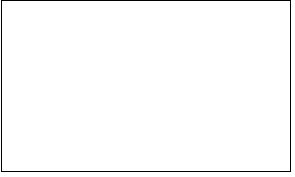
\includegraphics{figs/cas-grabs.pdf}
% \end{graphicalabstract}

% \begin{highlights}
% \item Research highlights item 1
% \item Research highlights item 2
% \item Research highlights item 3
% \end{highlights}

\begin{keywords}
    Quantum Key Distribution (QKD)\sep E91 protocol \sep Entanglement \sep CHSH inequality \sep Steganography \sep ChaCha20-Poly1305 \sep Hashing \sep Secure Hash Algorithm (SHA) \sep Encryption \sep Decryption
\end{keywords}


\maketitle


\section{Introduction}
The simplest, as well as the most important, form of exchange for human beings is verbal communications. The invention of the Telephone by Alexander Graham Bell in 1876 transformed the verbal communication demography - making the transmission of human voice, which are essentially audio signals, over long distances possible. In the subsequent centuries, technological improvements has broadened the scope of audio transmission. With the rise of the Internet, the amount of information exchanged through audio signals increased rapidly. This increase number audio transmission resulted in the development of different encryption techniques and cryptographic algorithms. The most popular among these algorithms are the symmetric AES and the asymmetric RSA encryption schemes. AES \cite{rijmen2001advanced} is a block cipher scheme that utilizes multiple matrix operation to encrypt and decrypt data using the same key. Without any knowledge of the cipher key, it is computationally infeasible to reverse the orations performed during encryption. RSA \cite{rivest1978method}, on the other hand, utilizes prime number factorization to generate public-private key-pairs for each user that are used to encrypt and decrypt data. The security of the RSA scheme relies on the insane amount of computational power required to obtain the private key from a public through prime number factoring.

However, with the advent of Quantum Computers with increasing number of functional qubits, these classical cryptography and encryption schemes face an imposing threat \cite{bernstein2017post}. In 1996, Lov K. Grover proposed an algorithm to search an unordered database of size $N$ using $\sqrt{N}$ quantum queries \cite{grover1996fast}. Using Grover's algorithm, the number of trials required to brute-force a key of length $k$ reduces from $2^{k}$ to $2^{k/2}$. This reduction in number of brute-force trials effectively reduces the security level of symmetric encryption schemes such as AES \cite{Daemen2002}. For example, the AES-128 encryption scheme with a pre-quantum security level of 128 reduces to a post-quantum security level of 64, which is much easier to brute-force. In 1994, P.W. Shor presented a quantum algorithm that can quickly find the prime factorization of any positive integer $N$ \cite{Shor1997}. As the security of the RSA algorithm relies on the arduousness of prime number factorization to derive private key from public key, it is currently facing an existential threat due to the exponential speed of Shor's algorithm. It is estimated that the time complexity for Shor's algorithm is $\mathcal{O}(72(log(N))^{3})$, as opposed to $\mathcal{O}(N^3)$ for classical computers.

\subsection{Current Challenges}
To address these arising challenges, new research is being done on the field of quantum augmented communication systems. These systems exploits the principles of quantum mechanics to attain secure data transmission. One of the most promising area of research in the field of quantum communications is Quantum Key Distribution (QKD). QKD protocols works by establishing a secure cryptographic key between two users over an insecure channel \cite{alleaume2014using}. QKD employ properties unique to quantum mechanics, such as the no-cloning theorem \cite{buvzek1996quantum} and the uncertainty principle \cite{sen2014uncertainty}, that ensures the detection of any eavesdropping attempts and thereby guarantees the security of the key. However, QKD itself does not provide security on its own, rather it facilitates the establishment and secure exchange of secret keys that are subsequently used by other cryptographic algorithms and encryption techniques to secure the transmitted information. In addition, the applicability of QKD is restricted by a few practical challenges such as slow key generation, vulnerability to noise, limited operational distance etc. In resemblance, the research being done on the field of steganography heralds the emergence of an effective information concealing technique to obscure sensitive information within seemingly harmless transmission. Steganography is the technique of hiding secret massage within another massage in such a manner that it is not discernible that a secret message is embedded \cite{Kahn1996}. However, the security of any steganographic technique is heavily dependent on the strength of cryptographic technique employed to encrypt the data \cite{anderson1998limits}. In summary
\begin{itemize}
    \item QKD facilitates secure sharing of encryption keys, but secure data transmission requires classical encryption systems.
    \item In spite of providing improved security, the real-life implementation of QKD is confined due to some practical challenges such as noise vulnerability, slow key generation etc.
    \item The security of steganography is dependent on the employed encryption scheme. If the encryption scheme is compromised, data security is in risk.
    \item Hybrid systems combining classical and quantum cryptography methods defend against different types of attacks but it complicates the system design and implementation.
\end{itemize}
\subsection{Proposed Solution}
The new vulnerabilities in secure data transmission due to quantum computer and the need to oppose them have been the motivation for our research. With the advancement in quantum computing technology, it is imperative to devise innovative cryptographic techniques that can keep the data secure in the prospect of an attack from these powerful computers. It is our aim to develop a vigorous solution for secure data communication by combining the strength of quantum communication with hash function, classical encryption and steganography. Hence, the objective our experimental work is to investigate the viability and credibility of integrating encrypted steganographic techniques with quantum protocols, specifically QKD, to strengthen the security and resilience of audio communication. This innovative amalgamation of steganography and quantum communication embodies a significant furtherance in the field, providing an exceptional and optimistic approach to secure data transmission.

This paper introduces a novel approach to reinforce the security of digital audio communication by combining the competency of QKD, classical encryption schemes and steganography. A high-level outline of our proposed solution is as follows --
\begin{itemize}
    \item \textbf{Secure Key Generation and Distribution:} Utilizing the E91 QKD protocol proposed by Artur K. Ekert in 1991 \cite{Ekert1991}, a shared cryptographic key with enhanced security against quantum threats is generated.
    \item \textbf{Key Derivation:} Employing the Secure Hashing Algorithm-3 (SHA3-256) \cite{dworkin2015sha}, the QKD-generated key is hashed to produce a fixed-length, high-entropy key for symmetric encryption.
    \item \textbf{Steganography:} Using Least Significant Bit (LSB) substitution steganography, an audio signal is hidden inside another audio signal \cite{cvejic2002increasing}.
    \item \textbf{Symmetric Encryption with Authentication:} The ChaCha20-Poly1305 AEAD (Authenticated Encryption with Associated Data) algorithm \cite{rfc7539} - which combines the stream cipher scheme, ChaCha20 \cite{bernstein2008chacha} with the message authentication code, Poly1305 \cite{bernstein2005poly1305} - the steganographic audio is encrypted. The encrypted audio is bundled with a message authentication tag, which is used for authentication and integrity verification.
\end{itemize}
% Our system utilizes the E91 QKD protocol proposed by Artur K. Ekert in 1991 \cite{Ekert1991} to generate a shared key with increased security, which is then hashed to produce a fixed-length (256 bits), high-entropy key that is suitable for symmetric encryption by employing the Secure Hashing Algorithm-3 (SHA3-256) \cite{dworkin2015sha}. We inspect the use of ChaCha20-Poly1305 authenticated encryption with associated data (AEAD) algorithm \cite{rfc7539} - which combines the stream cipher scheme, ChaCha20 \cite{bernstein2008chacha} with the message authentication code, Poly1305 \cite{bernstein2005poly1305} - to encrypt the steganographic audio. We performed least significant bit (LSB) substitution steganography to hide an audio signal inside another audio signal \cite{cvejic2002increasing}. 
The incorporation of QKD with classical symmetric encryption addresses various security concernment, providing protection against both classical and quantum threats.
\subsection{Paper Organization}
Our paper is organized is as follows - Section \ref{sec:relatedWorks} demonstrates the present sate of the field through the review of existing research and their development, laying the foundation for our our proposed scheme. Section \ref{sec:preliminaries} describes the foundational concepts of our proposed schemes. Section \ref{sec:methodology} describes the proposed methodology, presenting a detailed piecemeal explanation of our proposed architecture. Section \ref{sec:implementation} delves into the detailed description of our implementation. In section \ref{sec:analysis}, we present the analysis methods as well as the findings. Section \ref{sec:discussion} explore deeper into an extensive analysis of the results, construing the findings and excerpting key insights. Finally, section \ref{sec:conclusion} concludes the paper by indicating the direction of future work, highlighting the potential application and extension of our research.
% The Elsevier cas-sc class is based on the
% standard article class and supports almost all of the functionality of
% that class. In addition, it features commands and options to format the
% \begin{itemize} \item document style \item baselineskip \item front
% matter \item keywords and MSC codes \item theorems, definitions and
% proofs \item lables of enumerations \item citation style and labeling.
% \end{itemize}

% This class depends on the following packages
% for its proper functioning:

% \begin{enumerate}
% \itemsep=0pt
% \item {natbib.sty} for citation processing;
% \item {geometry.sty} for margin settings;
% \item {fleqn.clo} for left aligned equations;
% \item {graphicx.sty} for graphics inclusion;
% \item {hyperref.sty} optional packages if hyperlinking is
%   required in the document;
% \end{enumerate}  

% All the above packages are part of any
% standard \LaTeX{} installation.
% Therefore, the users need not be
% bothered about downloading any extra packages.
\section{Related Works}
\label{sec:relatedWorks}
Post-Quantum cryptography (PQC), also known as Quantum resistant Cryptography, is designed to stave off attacks
by both classical and quantum computers. In other words, to design a dependable and future-proof data communication
system, a blending of Classical Cryptography and Quantum Cryptography is imperative. One such type of blending
could be combining some form of symmetric encryption with quantum key distribution (QKD), as explored in this research.

Classical cryptography -- based on the hardness of mathematical problems and computation complexity -- has been used to secure information and communication for decades. The classical cryptographic techniques include Symmetric Encryption techniques such as Advanced Encryption System(AES), Data Encryption Standard (DES); Asymmetric key algorithms such as Rivest-Shamir-Adleman(RSA), Elliptic Curve Cryptography (ECC) and Hash Functions. These classical cryptography techniques could be the focus of brute force attacks, as they are not capable enough of handling the quantum attacks. To address this vulnerability, the algorithms of Post Quantum Cryptography was proposed -- which are strong, reliable and secure against the quantum attacks \cite{sharma2023post}.

E91 and BB84 are the methods of Quantum Key Distribution (QKD) based on the completeness of quantum mechanics. BB84 is the first QKD protocol, relying on the Heisenberg uncertainty principle and the no-cloning theorem.On the other hand, E91 is an entanglement based protocol basically generalized from of Bell's theorem. The users (Alice and Bob) can easily detect the eavesdropping attempt checking the Bell's inequality by using this protocol \cite{Ekert1991}. Among them, E91 is considered as safer and reliable though it faces some technical difficulties \cite{alvarez2016comparison}.

Hash functions are frequently used in modern cryptography in order to ensure authentication of the digital communication system. It takes an arbitrary length input and produces a fixed sized hashed value where any small changes in input results in an alteration of the hashed value. SHA-0, SHA-1, SHA-2, SHA-3 are the dedicated hash functions of the SHA family \cite{madhuravani2013cryptographic}. Among them, the SHA-3 family is based on permutation having an extendable output function. SHA3-224, SHA3-256, SHA3-384, SHA3-512 are known as cryptographic hash functions. SHA-3 provides resistance to collision, preimage and second preimage attacks which ensures the security attacks such as digital signature generation and verification, key derivation and pseudorandom bit generation  \cite{dworkin2015sha}.

Steganography is a common practice of hiding information. The main purpose of steganography is to secure the information so that it is completely undetectable through human senses \cite{amin2003information}. There are many types of steganography using different types of cover objects such as text \cite{yang2018rnn}, audio \cite{jayaram2011information}\cite{hemeida2021comparative}\cite{djebbar2012comparative}, video, images (2D and 3D) \cite{farrag2020secure} and information matrices \cite{mashaly2019multiple}. Due to their high level of data transmission rate and redundancy, digital audio signal are highly suitable for steganography \cite{singh2014survey}. Some of the audio stenographic process include LSB codding, Parity codding, Phase codding, Spread spectrum, Echo hiding. Among them, LSB is comparatively better as it increases robustness against noise addition and MPEG compression, high capacity and simplicity \cite{cvejic2004increasing}\cite{jayaram2011information}. When QKD protocols are combined with this, it improves more data security. using  Bernstein-Vazirani algorithm and the BB84 protocol, it generates a secret key to ensure only authorized access to quantum messages. This quantum steganography method increases hidden channel capacity, resists attacks like intercept-resend, and reduces message detectability by using more Bell states and random information distribution \cite{yalla2022novel}.

ChaCha, a variant of Salsa20, represent the ChaCha family of stream ciphers, which improves upon the previous Salsa20 design. It increases the resistance to cryptoanalysis by improving the diffusion per round while maintaining performance. It also achieves better software speed compared to Salsa20 in certain platforms due to its efficient design that allows for SIMD operations \cite{bernstein2008chacha}. ChaCha is a robust alternative to Salsa20, with enhancements that could make it preferable for various cryptographic applications.

The Poly1305 is a specific type of MAC(Message Authentication Protocol) which is a cryptographic tools used to verify the integrity and authenticity of a message \cite{bernstein2005poly1305}. It computes a 16-byte authenticator for variable-length messages using a 32-byte secret key, which includes a 16-byte key derived from some symmetric encryption and a 16-byte additional randomly generated key which helps in high-speed computations and making it suitable for various applications \cite{bernstein2005poly1305}. The probability of successful attack is also very low due to the uniqueness of nonces and the unpredictability of keys. For all the reasons, it is used widely for network protocols and secure communications.
\subsection{Novel Contributions to Existing Literature Gap}
The mentioned works offer valuable contributions, but they all have shortcomings as well. QKD by itself can not
provide any data security. Classical cryptography along with hash function as an integrity verifier provides good data
security, but this method is not competent enough to stave off quantum attacks. The consolidation of quantum
and classical cryptography offers a promising avenue for reinforcing security, as the combined strengths of these two
approaches can lead to more robust and resilient cryptographic systems. To that end, we introduce a cryptography
scheme combining Quantum Key Distribution and Classical cryptography, added with Steganography technique. This
mixture of different types of information-securing techniques provides a system that is resilient against both classical
and quantum attacks while providing efficient data security.   Our main contribution can be summarized as follows -
\begin{itemize}
    \item Proposed an original architecture that successfully combines E91 QKD protocol, ChaCha20-Poly1305 AEAD and audio steganography using LSB.
    \item Utilized E91 as the key distribution protocol which employs principles of quantum mechanics for secure key exchange.
    \item Assimilated audio steganography using LSB substitution into the architecture to augment the security and robustness of the overall system.
    \item Assessed the performance and reliability of the proposed scheme by measuring the security through end-to-end encryption.
\end{itemize}
\section{Preliminaries}
\label{sec:preliminaries}
In this section, we present the primary concepts employed in our methodology. We start with the quantum key distribution (QKD) protocol proposed by Artur Ekert in 1991, commonly known as the E91 key distribution protocol. Protected by Bell's inequality, E91 protocol provides a secure method of sharing generated key pairs. Then we proceed to the SHA3 family of hashing algorithms, specifically the SHA3-256 function, which can produce a unique 256-bit long hexstream for an input of any length. Next, we introduce the ChaCha20-Poly1305 AEAD, which combines the strong yet simple ChaCha20 stream cipher with Poly1305 MAC. Finally, we discuss the LSB steganography algorithm, which is essentially a technique of hiding an audio signal in the least significant bits of another, larger audio.
\subsection{Ekert 91 Protocol}
\label{sec:e91}
The E91 protocol is a quantum key distribution (QKD) scheme that uses entangled photon pairs and the violation of Bell's inequality to securely distribute cryptographic keys between two parties, typically referred to as Alice and Bob. The E91 protocol, based on the principles of quantum mechanics and entanglement, allows secure key distribution between two parties, Alice and Bob. The steps are as follows:
\begin{enumerate}
    \item Creating Entangled Pairs: Either alice or bob or any other third party, Charlie, can initiates the process by generating pairs of strongly entangled quantum particles (Bell states). These states ensure that the measurements on the particles are perfectly correlated. There are four Bell states, which are below:
          \[\ket{\Phi^{+}}=\frac{1}{\sqrt{2}}(\ket{00}+\ket{11}),\ket{\Phi^{-}}=\frac{1}{\sqrt{2}}(\ket{00}-\ket{11})\]
          \[\ket{\Psi^{+}}=\frac{1}{\sqrt{2}}(\ket{01}+\ket{10}),\ket{\Psi^{-}}=\frac{1}{\sqrt{2}}(\ket{01}-\ket{10})\]
          For notions such as $\ket{01}$ and $|\ket{11}$, the first digit in brackets refers to the first qubit, and the second digit refers to the second qubit.

    \item Sharing the Particles: After generating the entangled pairs, Charlie sends one particle of each pair each to Alice and the other to Bob or if they produced entangled qubits without the help of third party then they will send one particle to another.
    \item Performing Measurements: Alice and Bob, located far apart, independently measure their received particles using quantum measurement tools. Their devices are configured with randomly chosen azimuthal angles e.g.  \[
              \varphi_{A_1} = 0, \quad \varphi_{A_2} = \frac{\pi}{2}, \quad \varphi_{A_3} = \frac{\pi}{4} \quad \text{for Alice;}
          \]

          \[
              \varphi_{B_1} = 0, \quad \varphi_{B_2} = \frac{3\pi}{2}, \quad \varphi_{B_3} = \frac{\pi}{4} \quad \text{for Bob.}
          \]

          The outcomes (0 or 1) are inherently random due to quantum principles.
          Figure~\ref{fig:mesurement_direction} shows the measurement direction:

          \begin{figure}[pos=h]
              \centering
              \includesvg[width=0.75\textwidth]{measurement.svg}
              \caption{Measurement Direction for Ekert Protocol}
              \label{fig:mesurement_direction}
          \end{figure}

    \item Comparing Results:  Alice and Bob will share their measurement bases over a classical channel. They discard results where their measurement angles differed and keep only those whose bases are aligned. This filtered data forms the raw material for their shared key.
    \item Building the Shared key: For the matching bases, Alice and Bob use their correlated outcomes to construct an identical secret key. This key is a binary sequence that is used to securely encrypt/decrypt messages.
    \item Checking for Eavesdroppers: The protocol's security depends on the quantum entanglement. If an eavesdropper intercepts the particles, the entanglement is disrupted, altering the expected correlations. By testing a subset of their results, Alice and Bob can detect anomalies. If inconsistencies arise, they abort the key and restart the process.
\end{enumerate}

Alice and Bob can detect the presence of Eve using two steps. The first step is to check if, after measurement, they find that the measurement results differ despite using the same corresponding bases. They can also detect anomalies using the CHSH inequality test. If the measurement result don't violate CHSH inequality, then they can assume that there was an anomaly.
The CHSH inequality quantifies correlations between two spatially separated particles measured in different bases. For an entangled pair, if measurements on the first particle are labeled with settings A and a (yielding outcomes $ \pm 1 $), and those on the second particle use settings B and b (yielding outcomes $ \pm 1 $), the CHSH parameter S is defined as:
\begin{equation}
    S = A(B - b) + a(B + b)
\end{equation}
Classically, the absolute average value is given by:
\[
    |\langle S \rangle| \leq 2 \quad \text{or} \quad \pm 2.
\]
It is bounded by 2, as one of the terms \( (B \pm b) \) necessarily cancels out, leaving \( S = \pm 2 \).
Expanding S in terms of A, a, B and b results in:
\[
    \left| \langle S_1 \rangle \right| = \left| \langle AB \rangle - \langle Ab \rangle + \langle aB \rangle + \langle ab \rangle \right| \leq 2.
\]

Remarkably, quantum mechanics predicts violations of these classical bounds. Entangled particles, such as those in Bell states, exhibit stronger correlation due to nonlocal quantum interactions. When measured in specific non-commuting bases the CHSH parameter can reach
\[
    \left| \langle S \rangle \right| = 2\sqrt{2} \approx 2.828 \quad \left| \langle S \rangle \right|
\]
In our experiment, we expect to obtain a CHSH value close to \( 2\sqrt{2} \); otherwise, we can claim that there were anomalies/eavesdroppers in the channel.
\subsection{SHA3 -- 256 Hash Function}
\label{sec:sha3}
SHA-3 is the latest member \cite{nistHashFunctions} of the Secure Hash Algorithm (SHA) family of cryptographic hash functions. Based on the K\textsc{eecak} algorithm \cite{Bbbbbbb2011}, the SHA-3 standard differs fundamentally from its MD-5 \cite{rivest1992md5} like structured predecessors -- SHA-1 and SHA-2 \cite{penard2008secure}. In its essence, the SHA-3 standard is a hash function, that is, for any length of binary data input, there is an output of fixed length. The output is called the \textit{digest} or \textit{hash value}. Depending on the digest length, the four hash functions are called SHA3-224, SHA3-256, SHA3-384 and SHA3-512. The suffixes after the dash indicate the fixed length of the digest, for example, SHA3-256 -- which is of interest to our methodology -- produces 256 bits long digest. As the digest length is constant irrespective of input length, SHA3 is ideal for integrity and signature verification, as well as password hashing, that is not storing password in clear-text format, rather storing the hash of the password for verification.

SHA-3 works by using the sponge construction \cite{keccakKeccakTeam}. Here, data is "absorbed" into the sponge and the result is "squeezed" out, as sown in Figure \ref{fig:sponge}. For an input bit string $N$, a padding function $pad$, and a permutation function $f$ yields the sponge construction $Z=\text{sponge}[f,pad,r](N,d)$. Here, the permutation function $f$ operates on a bit block of width $b$, rate $r$ and yields and output of length $d$. From the sponge construct, we have capacity $c=b-r$ and digest $Z$ of length $b$. The block permutation $f$ is Keccak-f[1600] that utilizes XOR, AND and NOT operations. It is defined for any power-of-two word size, $w=2^l$. The basic block permutation function consists of $12+2l$ rounds of five steps: $\theta$ (parity computation), $\rho$ (bitwise rotation), $\phi$ (permutation), $\chi$ (bitwise combination) and $\iota$ (XOR).

\begin{figure}[pos=h]
    \centering
    \includesvg[width=0.75\textwidth]{SpongeConstruction.svg}
    % 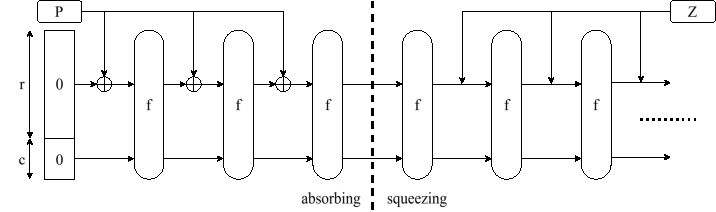
\includegraphics[width=0.75\textwidth]{SpongeConstruction.pdf}
    \caption{The sponge construction for SHA-3.}
    \label{fig:sponge}
\end{figure}

The process of retrieving the digest $Z$ from input $N$ is described below --
\begin{itemize}
    \item The input $N$ is padded using the padding function, $pad$. This yields in a padded bit strength $P$ the length of which is devisable by $r$ ($n=\text{len}(P)/r$).
    \item $P$ is broken into $n$ consecutive pieces, each piece of length $r$, so that $P \to P_{0},\ldots,P_{n-1}$
    \item State $S$ is initialized with sting of $b$ zero bits.
    \item The input is absorbed into the state: for each block $P_{i}$, \begin{itemize}
              \item $P_{i}$ is extended at the end by $c$ zero bits, so that the length is $b$.
              \item The resulting bit string is XORed with $S$.
              \item The block permutation $f$ is applied on the result, yielding a new state $S$.
          \end{itemize}
    \item $Z$ is initialized with empty string
    \item while \textit{length}$(Z)<d$:\begin{itemize}
              \item The first $r$ bits of $S$ is appended to $Z$.
              \item \textit{if} $(\textit{length}(Z)<d)$, apply $f$ to $S$, yielding a new $S$.
          \end{itemize}
    \item $Z$ is truncated to $d$ bits.
\end{itemize}

For example, for the following binary stream, \[N=00100000010001010100000110011000010001001111101010000001100011001111101101011110\]
the digest is $43b3d090d2aebb7790183e58808b71fe890858b5ca3fd308efb2aeba2fde0b71$
\subsection{ChaCha20-Poly1305}
\label{sec:chacha20}
ChaCha20-Poly1305 is an authenticated encryption with associated data (AEAD) algorithm that provides a comparatively fast software performance. It is typically faster than AES-GCM (Galois/Counter Mode) in the absence of hardware acceleration \cite{rfc7539}. This algorithm combines the ChaCha20 stream cipher \cite{bernstein2008chacha} and the Poly1305 \cite{bernstein2005poly1305} universal hash family that acts as message authentication code -- both of which was developed independently by Daniel J. Bernstein.

A stream cipher is a symmetric key cipher, that is an encryption and decryption algorithm, that combines plaintext data with a pseudorandom keystream \cite{robshaw1995stream}. Stream ciphers works by encrypting each plaintext digit one at a time with the corresponding keystream digit, as opposed to block ciphers where blocks of plaintext with a certain length is encrypted with the keystream. In 2008, Bernstein proposed the ChaCha family of stream ciphers, a successor to the Salsa20 stream cipher \cite{bernstein2005salsa20} proposed by Bernstein in 2005. ChaCha was proposed as an alternative to Salsa20 \cite{bernstein2008chachaFamily} with slightly better performance. Similar to it's predecessor, the initial state of ChaCha is 512-bit long -- made up of a 128-bit constant, a 256-bit key, a 64-bit counter and a 64-bit nonce. The 128-bit constant is usually \textit{"expand 32-byte k"}. This 512-bit long input is arranged in a $4\times4$ matrix where each entry is a 32-bit word. The matrix arrangement is shown bellow --
\begin{equation}\label{initialState}
    \left[
        \begin{array}{cccc}
            \text{Constant}[0] & \text{Constant}[1] & \text{Constant}[2] & \text{Constant}[3] \\
            \text{Key}[0]      & \text{Key}[1]      & \text{Key}[2]      & \text{Key}[3]      \\
            \text{Key}[4]      & \text{Key}[5]      & \text{Key}[6]      & \text{Key}[7]      \\
            \text{Counter}[0]  & \text{Counter}[1]  & \text{Nonce}[0]    & \text{Nonce}[1]
        \end{array}
        \right]
\end{equation}
The core operation of ChaCha, and it's predecessor Salsa20, is the quarter-round \text{\ttfamily{QR(a,b,c,d)}}. ChaCha uses 4 additions, 4 XORs and 4 rotations to update 4 32-bit state words -- \text{\ttfamily{a,b,c,d}}. The update procedure is as follows --
\begin{lstlisting}[basicstyle=\ttfamily,frame=none]
    a += b; d ^= a; d <<<= 16;
    c += d; b ^= c; b <<<= 12;
    a += b; d ^= a; d <<<=  8;
    c += d; b ^= c; b <<<=  7;
\end{lstlisting}

\noindent If the elements of matrix \ref{initialState} is indexed from 0 to 15
\[\left[
        \begin{array}{cccc}
            0  & 1  & 2  & 3  \\
            4  & 5  & 6  & 7  \\
            8  & 9  & 10 & 11 \\
            12 & 13 & 14 & 15
        \end{array}
        \right]\]
a double round in ChaCha is defined as --
\begin{lstlisting}[basicstyle=\ttfamily,frame=none]
    // Odd round
    QR(0, 4,  8, 12) // column 1
    QR(1, 5,  9, 13) // column 2
    QR(2, 6, 10, 14) // column 3
    QR(3, 7, 11, 15) // column 4
    // Even round
    QR(0, 5, 10, 15) // diagonal 1 (main diagonal)
    QR(1, 6, 11, 12) // diagonal 2
    QR(2, 7,  8, 13) // diagonal 3
    QR(3, 4,  9, 14) // diagonal 4
\end{lstlisting}
ChaCha20 uses 10 iterations of the double round -- an overall of 20 rounds. Hence the name ChaCha20.

\begin{figure}[pos=h]
    \centering
    \includesvg[width=0.75\textwidth]{ChaCha_Cipher_Quarter_Round_Function.svg}
    \caption{The ChaCha quarter-round function.}
\end{figure}

Each word is updated twice in ChaCha20's quarter rounds, as opposed to Salsa20 where each word is updated only once. This results in an average of $12.5$ output bits to change in each quarter round of ChaCha20, while the Salsa20 quarter-round changes 8 output bits. Although the ChaCha quarter round contains the same number of adds, xors, and bit rotates as the Salsa20 quarter round, it is slightly faster because two of the rotate functions are multiples of 8, allowing for a small optimization for x86 and other architectures.

After the 10 iterations, a keystream, $K$ is generated which is XORed with the message stream, $M$, to produce the cipher, C.
\[C = K \oplus M\]
For decryption, the keystream, $K$, is XORed with the cipher, $C$, to retrieve the message, $M$.
\[M = C \oplus K\]


A hash function is a special mathematical function that can data of arbitrary size to constant-sized values. The output of a hash function is called hash digest or simply hashes. A unique property of most hash functions is their ability to generate unique digests for each unique inputs. This makes hash functions invaluable for authentication and data integrity verification.In 2002, Bernstein designed the Poly1305 universal hash function, which was intended to provide a message authentication code to authenticate a message using a shared secret key \cite{bernstein2005protecting}. The original implementation of Poly1305 was in 2005 when Poly1305 hash was combined as a Carter-Wegman authenticator \cite{carter1981new} with AES-128 to authenticate encrypted messages.

Poly1305 provides a 128-bit long authentication tag from a 256-bit long one-time key, and a message of arbitrary length. The key has two portions -- $r$ and $s$. It is recommended that the pair $(r,s)$ to be unique. The first portion, $r$, is a 128-bit key produced form a symmetric encryption scheme similar to AES. The later portion, $s$, is a 128-bit long integer arranged as a 16-octet little-endian format. It is required that --
\begin{itemize}
    \item $r[3], r[7], r[11]$ and $r[15]$ have their top four bits clear (to be in $\{0,1,\ldots,15\}$).
    \item $r[4], r[8]$ and $r[12]$ have their bottom four bits clear (to be in $\{0,4,8,\ldots,252\}$).
\end{itemize}

Each message is required to accompanied by a 128-bit Nonce generated from the accompanying encryption scheme. The process of producing the authenticator tag from the message and the key are briefly outlined here --
\begin{itemize}
    \item A variable called the "accumulator" is initialized with zeros
    \item The message is divided into 128-bit long blocks. Each block is read in little-endian sequence.
    \item Each block is appended by 1 byte so that each block is 136-bit long. If any of the block is not 136-bit long (usually the last block), the block is padded with zeros to make it of proper length.
    \item Each 136-bit long message block is multiplied with a clamped value $r$ and the multiplication result is added to the accumulator.
    \item The value stored in the accumulator is reduced using $mod(2^{128})$ and the reduced value is stored in the accumulator.
    \item When the whole message is converted, the value in the accumulator is added to $s$.
    \item From the result, the 128 least significant bits are formatted in little-endian format to produce the tag.
\end{itemize}

The ChaCha20-Poly1305 AEAD adopted for Internet Engineering Task Force (IETF) \cite{rfc8439} and subsequently as the standard for Transport Layer security (TLS) \cite{rfc7905} and the OpenBSD Secure Shell (OpenSSH) \cite{miller2015chacha20} is slightly different from the original structures proposed by Daniel J. Bernstein. To be precise, the ChaCha20 symmetric encryption is slightly modified. As opposed to a 64-bit Nonce, the modified ChaCha20 has a 96-bit long Nonce. The modified matrix is shown below --
\begin{equation}\label{initialStateMod}
    \left[
        \begin{array}{cccc}
            \text{Constant}[0] & \text{Constant}[1] & \text{Constant}[2] & \text{Constant}[3] \\
            \text{Key}[0]      & \text{Key}[1]      & \text{Key}[2]      & \text{Key}[3]      \\
            \text{Key}[4]      & \text{Key}[5]      & \text{Key}[6]      & \text{Key}[7]      \\
            \text{Counter}[0]  & \text{Nonce}[0]    & \text{Nonce}[1]    & \text{Nonce}[2]
        \end{array}
        \right]
\end{equation}

The remaining portions of the ChaCha20 scheme remains unaltered. The same is true for the Poly1305 authenticator. A high level overview of this modified ChaCha20 encryption and Poly1305 authenticator tag generation is outlined below --
\begin{itemize}
    \item A 256-bit long string is used as key for the ChaCha20 key along with a unique 96-bit long Nonce.
    \item Using the key and the nonce, the ChaCha20 block function is activated, which produces a 512-bit state.
    \item The first 256 serialized bits of the 512-bit state is taken as the Poly1305 key -- the 128 bit as $r$ and the next 128 bit as $s$.
    \item The 512-bit state is serialized in little-endian format to produce a keystream.
    \item The keystream is XORed with the message to produce the ciphertext.
    \item The Poly1305 function is called with the ciphertext and the previously derived key as input to produce the authenticator tag.
\end{itemize}
The output from the AEAD is the concatenation of the following --
\begin{itemize}
    \item A ciphertext which is as long as the plaintext message.
    \item A 128-bit authenticator tag, generated by the Poly1305 function.
\end{itemize}
\subsection{LSB Steganography}
\label{sec:steganography}
Steganography is the process where we don't encrypt the secrete message, rather we hide it in another file. Trough this process we can hide different types of secrete data like text, image, video, audio etc. within cover data which can also be in any different data types.\cite{jayaram2011information}\cite{hemeida2021comparative}
\begin{figure}[pos=H]
    \begin{center}
        \includesvg[width=0.6\textwidth]{steganographyApplication.svg}
        \caption{Steganography Application Scenario}
        \label{fig:stegoApplication}
    \end{center}
\end{figure}

In Audio Steganography secret message is hidden in cover audio but there is no much change in the cover audio because it is it use of the psycho-acoustical masking phenomenon of the human auditory system(HAS). There are different methods of steganography. Among them some notables are: LSB Coding, Parity Coding, Phase coding, Spread spectrum, Echo hiding etc.\cite{hemeida2021comparative} A very popular methodology among them is the LSB(Least Significant Bit) algorithm, which only replaces the least significant bits of the some of the bytes of the cover audio. Due to LSB substitution there is no much changes in the audio also.
\begin{figure}[pos=h]
    \begin{center}
        \includesvg[width=\textwidth]{embedStego.svg}
        \caption{Block Diagram of LSB Embedding implementation logic.}
        \label{fig:stegoEmbed}
    \end{center}
\end{figure}

LSB encoding embeds secret audio by replacing the least significant bits of carrier audio frames with bits from the secret audio. First, the carrier and secret audio are checked for compatibility in terms of channels and sample width. The secret audio frames are resized to fit the carrier's capacity. A mask is applied to clear the carrier's LSBs, which are then replaced with shifted bits from the secret audio. The result is a modified carrier audio with embedded data, saved as a new file.
\begin{figure}[pos=h]
    \begin{center}
        \includesvg[width=\textwidth]{extractStego.svg}
        \caption{Block Diagram for Steganalysis for extracting the embedded data.}
        \label{fig:stegoExtract}
    \end{center}
\end{figure}

Decoding isolates the embedded bits by applying a mask on the embedded audio and shifting these bits back to their original positions to reconstruct the secret audio. To improve quality, a low-pass filter reduces noise. The reconstructed audio is clipped to valid ranges and saved as the extracted secret.
\section{Methodology}
\label{sec:methodology}
\begin{figure}[pos=h]
    \begin{center}
        \includesvg[width=\textwidth]{methodology.svg}
        \caption{A high level overview of the proposed methodology}
        \label{fig:methodology}
    \end{center}
\end{figure}
The architecture that we proposed is a system that integrates E91 QKD protocol with classical cryptographic schemes and lsb steganography to ensure a heavily secure audio data encryption system. The system utilizes the E91 for QKD to generate and exchange the cryptographic keys called the Ekert key, SHA3 to derive a high-entropy 256-bit key from the Ekert key for ChaCha20-Poly1305 encryption and LSB substitution for steganography. The architecture ensures augmented data security through the combination of classical and quantum techniques. Figure \ref{fig:methodology} provides a high level overview of our proposed system.
\subsection{Initialization}
\label{sec:init}
As outlined by Ekert \cite{Ekert1991}, an entangled pair generator, referred to as Charlie, produces pairs of entangled qubits and shares them with Alice and Bob. The circuit shown in Figure \ref{fig:singlet} is used to produce the entangled qubit pairs. The circuit applied a Hadamard $(H)$ gate to put a qubit in superposition and a CNOT $(\oplus)$ gate to control the other qubit. Here, $qr_{0}$ and $qr_{1}$ denotes quantum registers, that is, qubits, while $cr$ denotes classical register.
\begin{figure}[pos=h]
    \centering
    \begin{quantikz}
        \lstick{$qr_{0}$} & \gate{H} & \ctrl{1} & \\
        \lstick{$qr_{1}$} & & \targ{} &  \\
        \lstick{$cr$}\setwiretype{c} & & &
    \end{quantikz}
    \caption{Singlet circuit for creating entanglement qubit pairs.}
    \label{fig:singlet}
\end{figure}
\subsection{Measurement}
\label{sec:measurement}
Alice and Bob independently create a random set of bases of length $n$. Using this set of random bases, Alice and Bob perform measurements on the qubits they received from Charlie. After the completion of the measurements, both parties share their measurement bases over an unsecured Classical Channel. Upon comparison of these measurement bases, the states that lack a common base are discarded. The result is a secret key called the Final Ekert Key that is shared between Alice and Bob. The measurement process is illustrated in Figure \ref{fig:combined}.
\begin{figure}[pos=h]
    \begin{center}
        \begin{quantikz}
            \lstick{$qr_{0}$} & \gate{H}\gategroup[2,steps=2,style={dashed,rounded corners}]{Charlie} & \ctrl{1} & & \gate{A}\gategroup[3,steps=1,style={dashed,rounded corners}]{Alice} \wire[d][2]{q} & & & \\
            \lstick{$qr_{1}$} & & \targ{} & & & & \gate{B}\gategroup[2,steps=1,style={dashed,rounded corners}]{Bob} \wire[d][1]{q} & \\
            \lstick{$cr$}\setwiretype{c} & & & & & & &
        \end{quantikz}
        \caption{Combined circuit for E91 QKD protocol}
        \label{fig:combined}
    \end{center}
\end{figure}
\subsection{Encryption key generation}
\label{sec:keyGen}
After the creation of the final Ekert key, Alice and Bob pass the key through the SHA3-256 hashing algorithm to generate another key of fixed length (256 bits) and high entropy. The use of the hashed key is instead of the original Ekert key provides an additional layer of security by obscuring the contents of the original key. If an eavesdropper gets hold of the hashed key, he/she will not be able distill the original key as the SHA3 hash function provides a vital protection against reverse calculation.

For 500 singlet states, we may get a key like the following --\\
$01011000100110100111011110111100001100111111000101110001100000011110111011000000100101110111$

\noindent The hash digest of this key is $486340cb54e65a96edc02257b48f3415a0c374f771871a4240ef8097cecdeec2$.

Similarly, for 128 singlet states, we may get a key like the following -- $0001001110110110111000101100$. \\
The hash digest of this key is $9e0ae69c28e4f4e8ba13e1c496fb237284df4e0b6540e168b18bec0cde9ee70f$.
\subsection{Steganographic embedding}
\label{sec:stegoEncode}
Prior encryption, the audio data is embedded in a cover audio using Steganography. The technique of Least Significant Bit (LSB) substitution is used to produce the stego audio, that is, the audio file created from the cover audio that hides the message audio. First, the message and the cover audio is checked for compatibility. Upon success, the cover audio frames are modified through masking, which clears the LSB of each frame. They are subsequently replaced by the bits of the message audio.
\subsection{Encryption and Authenticator generation}
\label{sec:chacha20poly1305encryption}
The hashed key generated in \ref{sec:keyGen} is used to encrypt the stego audio generated in \ref{sec:stegoEncode}. The encryption process is accompanied by the generation of an authenticator tag. The ChaCha20-Poly1305 AEAD is used to perform the encryption. The high-level over view of the process is shown in Figure \ref{fig:chacha20poly1305encryption}.
\begin{figure}[pos=h]
    \centering
    \includesvg[width=0.5\textwidth]{chacha20poly1305.svg}
    \caption{ChaCha20-Poly1305 Encryption and Authenticator tag generation.}
    \label{fig:chacha20poly1305encryption}
\end{figure}

The 256-bit key derived from the SHA3-256 hashing algorithm is input along with a 96-bit Nonce and a 8-bit Counter to the ChaCha20 Block function. The function generates a 512-bit state after 20 rounds, which is serialized into a keystream in little-endian format. The first 256-bits of the keystream is input to the Poly1305 hash function along with other associated data. The keystream is XORed with the stego audio to produce the encrypted audio. The encrypted audio is put into the Poly1305 hash function which produces a 128-bit long authenticator tag.
\subsection{Decryption and Authentication}
\label{sec:chacha20poly1305decryption}
The decryption process is the exact reverse of the encryption process. Similar to the encryption process, a 256-bit long key is derived from the shared Ekert key using the SHA3-256 hash function. The key is used to generate the ChaCha20 keystream, similar to the encryption process. The keystream is used in the Poly1305 hash function along with the received encrypted audio to generate a authenticator tag. The generated tag is compared with the received tag to verify the validity and integrity of the received data. Upon validation, the encrypted audio is XORed with the previously generated keystream to recover the stego audio.
\subsection{Steganography extraction}
\label{sec:stegoExtract}
The stego audio recovered in \ref{sec:chacha20poly1305decryption} is modified to isolate the cover audio and the message audio. As the least significant bits of each frame of the cover audio was replaced by the message audio bits, the LSBs of each frame was extracted in order to reconstruct the binary stream of the message audio. The reconstructed binary stream is modified according to bit-depth to form audio frames. From these frames the message audio is reconstructed.

In summary, Charlie creates entangled pairs of qubits which are shared with Alice and Bob. They perform measurements on the received qubits, resulting in the creation of the Final Ekert Key. This key is hashed using SHA3-256 to produce 256-bit high-entropy symmetric encryption key. Alice embeds the secret audio file in a cover audio file through LSB steganography. This embedded audio is encrypted using ChaCha20-Poly1305 AEAD, which uses the symmetric encryption key. The encrypted audio is decrypted by Bob using the same key through ChaCha20-Poly1305 decryption and authenticates the validity of the message. Finally, through LSB extraction, Bob reproduces the secret audio from the decrypted audio.
% \newpage
\section{Implementation Details}
\label{sec:implementation}
In the course of our research, we utilized an amalgamation of powerful tools and libraries in the pursuit of the effective implementation of our proposed scheme. The Qiskit SDK from IBM \cite{Wille2019IBMsQT} acted as one of the foundational columns of our research by enabling us to develop and simulate quantum circuits and thus properly implementing the E91 protocol. For our implementation, we specifically used Qiskit v0.39.2. Using Qiskit, we developed the singlet circuit for entangled pair generation \ref{fig:singlet}, the measurement circuits of Alice and Bob and the creation of the Final Ekert Key. The respective measurement circuits are shown in Figures \ref{fig:aliceMeasurements} and \ref{fig:bobMeasurements}.
\begin{figure}[pos=h]
    \begin{subfigure}[!h]{0.48\textwidth}
        \centering
        \begin{quantikz}
            \lstick{$qr_{0}$} & \gate{S} & \gate{H} & \gate{T} & \gate{H} & \meter{} \wire[d][2]{c} & \\
            \lstick{$qr_{1}$} & & & & & & \\
            \lstick{$cr$}\setwiretype{c} & & & & & &
        \end{quantikz}
        \caption{$W$ basis}
    \end{subfigure}
    \hfill
    \begin{subfigure}[!h]{0.48\textwidth}
        \centering
        \begin{quantikz}
            \lstick{$qr_{0}$} & \gate{H} & \ctrl{1} & \meter{} \wire[d][2]{c} & \\
            \lstick{$qr_{1}$} & & \targ{} & & \\
            \lstick{$cr$}\setwiretype{c} & & & &
        \end{quantikz}
        \caption{$X$ basis}
    \end{subfigure}
    \vfill
    \begin{subfigure}[!h]{\textwidth}
        \centering
        \begin{quantikz}
            \lstick{$qr_{0}$} & \meter{} \wire[d][2]{c} & \\
            \lstick{$qr_{1}$} & & \\
            \lstick{$cr$}\setwiretype{c} & &
        \end{quantikz}
        \caption{$Z$ basis}
    \end{subfigure}
    \caption{Alice's measurement circuits.}
    \label{fig:aliceMeasurements}
\end{figure}
\begin{figure}[pos=h]
    \begin{subfigure}[!h]{0.48\textwidth}
        \centering
        \begin{quantikz}
            \lstick{$qr_{0}$} & & & & & & \\
            \lstick{$qr_{1}$} & \gate{S} & \gate{H} & \gate{T^\dag} & \gate{H} & \meter{} \wire[d][1]{c} & \\
            \lstick{$cr$}\setwiretype{c} & & & & & &
        \end{quantikz}
        \caption{$V$ basis}
    \end{subfigure}
    \hfill
    \begin{subfigure}[!h]{0.48\textwidth}
        \centering
        \begin{quantikz}
            \lstick{$qr_{0}$} & & & & & & \\
            \lstick{$qr_{1}$} & \gate{S} & \gate{H} & \gate{T} & \gate{H} & \meter{} \wire[d][1]{c} & \\
            \lstick{$cr$}\setwiretype{c} & & & & & &
        \end{quantikz}
        \caption{$W$ basis}
    \end{subfigure}
    \vfill
    \begin{subfigure}[!h]{\textwidth}
        \centering
        \begin{quantikz}
            \lstick{$qr_{0}$} & & \\
            \lstick{$qr_{1}$} & \meter{} \wire[d][1]{c} & \\
            \lstick{$cr$}\setwiretype{c} & &
        \end{quantikz}
        \caption{$Z$ basis}
    \end{subfigure}
    \caption{Bob's measurement circuits.}
    \label{fig:bobMeasurements}
\end{figure}

The key was then zero padded to make it divisible by 8. The zero padded key was converted into a high entropy 256-bit long encryption key using PyCryptodome's \cite{pycryptodome} hash function -- specifically the SHA3-256 function, as stated in \ref{sec:keyGen}.

For our research, we used a single cover audio to hide two secret message audios using LSB steganography following the process detailed in \ref{sec:stegoEncode} using the computational tools and libraries provided by NumPy \cite{harris2020array}. For our cover audio, we chose \href{https://pixabay.com/music/beats-no-place-to-go-216744/}{No Place To Go}. The original audio was in \textit{.mp3} format. We converted it into \textit{.wav} format using FFmpeg \cite{newmarch2017ffmpeg} and stored it as \textit{cover.wav}. The waveform of the cover audio is shown in Figure \ref{fig:coverAudio}. For our secret audios, we chose \href{https://pixabay.com/music/future-bass-alone-296348/}{Alone} as secret audio 1 and \href{https://pixabay.com/music/future-bass-stylish-deep-electronic-262632/}{Stylish Deep Electronic} as secret audio 2. Similar to the cover audio, the secret audios were converted from \textit{.mp3} format to \textit{.wav} format using FFmpeg and was saved as \textit{secret1.wav} and \textit{secret2.wav}, respectively. Their respective waveforms are shown in Figure \ref{fig:secretAudio1} and \ref{fig:secretAudio2}.

\begin{figure}[pos=H]
    \begin{center}
        \begin{subfigure}[!h]{0.45\textwidth}
            \includesvg[width=\textwidth]{cover.svg}
            \caption{Waveform of Cover audio (\href{https://drive.google.com/file/d/13kdXTKmjT0xhZVx6o9LQ5Vw33wbg7ZUV/view?usp=drive_link}{\textit{cover.wav}.})}
            \label{fig:coverAudio}
        \end{subfigure}
    \end{center}
    \begin{subfigure}[!h]{0.45\textwidth}
        \begin{center}
            \centering
            \includesvg[width=\textwidth]{secret1.svg}
            \caption{Waveform of Secret audio 1 (\href{https://drive.google.com/file/d/18i7FJQoh4t5WSy7vJ1vKk0Vf5ALFBXbC/view?usp=drive_link}{\textit{secret1.wav}.})}
            \label{fig:secretAudio1}
        \end{center}
    \end{subfigure}
    \hfill
    \begin{subfigure}[!h]{0.45\textwidth}
        \begin{center}
            \includesvg[width=\textwidth]{secret2.svg}
            \caption{Waveform of Secret audio 2 (\href{https://drive.google.com/file/d/1-nvo0a90pLwNstRUYJz0A_JeYxTTvCC0/view?usp=drive_link}{\textit{secret2.wav}}).}
            \label{fig:secretAudio2}
        \end{center}
    \end{subfigure}
    \caption{Waveforms of Cover audio and Secret audios.}
\end{figure}

Using the LSB steganography technique, we embedded \textit{secret1.wav} and \textit{secret2.wav} inside \textit{cover.wav} and saved them as \textit{embedded1.wav} and \textit{embedded2.wav}. Their respective waveforms are shown in Figure \ref{fig:embeddedAudio1} and \ref{fig:embeddedAudio2}. From visual and auditory analysis of the waveforms, we found imperceptible differences between these three audio signals, indicating effective implementation of LSb steganography.
\begin{figure}[pos=h]
    \begin{subfigure}[!h]{0.45\textwidth}
        \begin{center}
            \centering
            \includesvg[width=\textwidth]{embedded1.svg}
            \caption{Waveform of Embedded audio 1 (\href{https://drive.google.com/file/d/1QLpjPCV-qFr1sKiN3rxpOOmUICOiu5hA/view?usp=drive_link}{\textit{embedded1.wav}}).}
            \label{fig:embeddedAudio1}
        \end{center}
    \end{subfigure}
    \hfill
    \begin{subfigure}[!h]{0.45\textwidth}
        \begin{center}
            \includesvg[width=\textwidth]{embedded2.svg}
            \caption{Waveform of Embedded audio 2 (\href{https://drive.google.com/file/d/1weMUGkD9NFAO6HAVIQ7LOt6ksLJKHcn6/view?usp=drive_link}{\textit{embedded2.wav}}).}
            \label{fig:embeddedAudio2}
        \end{center}
    \end{subfigure}
    \caption{Waveforms of Embedded audios produced through LSB Steganography.}
\end{figure}

The encryption key was used as the input key to PyCryptodome's ChaCha20-Poly1305 AEAD function in order to generate the cipher keystream as per the procedure stated in \ref{sec:chacha20poly1305encryption}. Using the keystream, the embedded audios, \textit{embedded1.wav} and \textit{embedded2.wav} was encrypted as ciphertext. From the the ciphertext, the authenticator tag was generated. The nonce used in producing the ciphertext, the ciphertext itself and the corresponding tag was stored in \textit{.bin} files, namely, \textit{encrypted1.bin} and \textit{encrypted2.bin}. The \textit{.bin} files were structured in such a way that the 96-bit nonce was followed by the ciphertext, which was in turn followed by the 128-bit tag. The waveforms of the encrypted audios are shown in Figure \ref{fig:encrypted1} and \ref{fig:encrypted2}.

\begin{figure}[pos=h]
    \begin{subfigure}[h]{0.45\textwidth}
        \begin{center}
            \includesvg[width=\textwidth]{encrypted1.svg}
            \caption{Waveform of Encrypted audio 1 (\href{https://drive.google.com/file/d/1fyl3awT4OiCKDLbgOBVyJiQFywCXubHJ/view?usp=drive_link}{\textit{encrypted1.wav}}).}
            \label{fig:encrypted1}
        \end{center}
    \end{subfigure}
    \hfill
    \begin{subfigure}[h]{0.45\textwidth}
        \begin{center}
            \includesvg[width=\textwidth]{encrypted2.svg}
            \caption{Waveform of Encrypted audio 2 (\href{https://drive.google.com/file/d/13Yfz3mYeFxycPza1hi8XbAg1jy4cI5Wr/view?usp=drive_link}{\textit{encrypted2.wav}}).}
            \label{fig:encrypted2}
        \end{center}
    \end{subfigure}
    \caption{Waveforms of the Encrypted audios produced by encrypting the Embedded audios.}
\end{figure}

The encrypted file was received by the intended recipient, who decrypted the file and authenticated it by comparing the received tag and the newly computed tag, as illustrated in \ref{sec:chacha20poly1305decryption}. Upon decryption and successful authentication, the audio was stored in \textit{.wav} files, namely, \textit{decrypted1.wav} and \textit{decrypted2.wav}, corresponding to \textit{embedded1.wav} and \textit{embedded2.wav}. The waveforms of these decrypted audios are shown in Figure \ref{fig:decrypted1} and \ref{fig:decrypted2}. Upon analyzing both visually and aurally, we found the decrypted audios, \textit{decrypted1.wav} and \textit{decrypted2.wav} to be indistinguishable from their embedded counterparts, \textit{embedded1.wav} and \textit{embedded2.wav}.

\begin{figure}[pos=h]
    \begin{subfigure}[h]{0.45\textwidth}
        \begin{center}
            \includesvg[width=\textwidth]{decrypted1.svg}
            \caption{Waveform of Decrypted audio 1 (\href{https://drive.google.com/file/d/1BbYutJlHVgVStUuAX9_TGZQJQnQrmKWd/view?usp=drive_link}{\textit{decrypted1.wav}}).}
            \label{fig:decrypted1}
        \end{center}
    \end{subfigure}
    \hfill
    \begin{subfigure}[h]{0.45\textwidth}
        \begin{center}
            \includesvg[width=\textwidth]{decrypted2.svg}
            \caption{Waveform of Decrypted audio 2 (\href{https://drive.google.com/file/d/1NXJOFLN7jP7fxDNhsJQ88p4ldTJE_9Pe/view?usp=drive_link}{\textit{decrypted2.wav}}).}
            \label{fig:decrypted2}
        \end{center}
    \end{subfigure}
    \caption{Waveforms of the Decrypted audios produced by decrypting the Encrypted audios.}
\end{figure}

From the decrypted audios, we extracted the secret audio as detailed in \ref{sec:stegoExtract}. The extracted audios was stored as \textit{extracted1.wav} and \textit{extracted2.wav}, corresponding to \textit{decrypted1.wav} and \textit{decrypted2.wav}. The waveforms of these audios are shown in Figure \ref{fig:extracted1} and \ref{fig:extracted2}. Visual analysis depicted a slight variation between original secret audios and extracted audios, that is, between \ref{fig:secretAudio1} and \ref{fig:extracted1} as well as \ref{fig:secretAudio2} and \ref{fig:extracted2}. This change was corroborated by the auditory analysis. Nevertheless, these slight variations did not make the extracted audio intelligible, rather, it felt like the amplitude of the audio signals was slightly decreased, proving an effective LSB steganographic extraction.

\begin{figure}[pos=h]
    \begin{subfigure}[h]{0.45\textwidth}
        \begin{center}
            \includesvg[width=\textwidth]{extracted1.svg}
            \caption{Waveform of Extracted audio 1 (\href{https://drive.google.com/file/d/12_0keSBukOVs4bYei2KcD-kNjAPxFFdQ/view?usp=drive_link}{\textit{extracted1.wav}}).}
            \label{fig:extracted1}
        \end{center}
    \end{subfigure}
    \hfill
    \begin{subfigure}[h]{0.45\textwidth}
        \begin{center}
            \includesvg[width=\textwidth]{extracted2.svg}
            \caption{Waveform of Extracted audio 2 (\href{https://drive.google.com/file/d/1Ikted9eaGw5HmMriXayIZHRsX-7acT6Z/view?usp=drive_link}{\textit{extracted2.wav}}).}
            \label{fig:extracted2}
        \end{center}
    \end{subfigure}
    \caption{Waveforms of the Extracted audios produced through LSB extraction.}
\end{figure}

All the audio waveforms shown in this section were generated using MATLAB \cite{MATLAB:R2016a}.
\section{Analysis}
\label{sec:analysis}
\subsection{Analysis of Encryption Properties}
With the help of the tools provided by NumPy, we calculated various properties of the encrypted audio signals obtained in the course of implementing our methodology. These properties ranges from entropy of the encrypted signal to sample change rate analysis.
\subsubsection{Entropy Analysis}
The randomness and unpredictability of a cipher can be measured by the Shanon entropy \cite{shannon1948mathematical}. In our scenario, the entropy of an encrypted audio signal is an indication of its unpredictability and randomness. The method of calculating entropy is as follows --
\begin{equation}
    H(x)=-\sum_{i=1}^{n}P(x_i)\log_{b}(P(x_i))
\end{equation}
Here, $H(x)$ is the entropy of the signal while $P(x_i)$ is the probability of the $i$th value of signal $x$. For a good encryption technique, it is desirable to have the entropy of the encrypted signal to be as close to $16$ as possible (for 16-bit audio signals). Table \ref{table:entropy} shows the entropy values of the two encrypted signals, as well as those of the embedded signals.
\begin{table}[pos=h]
    \begin{center}
        \caption{Entropy of original embedded audios before encryption, after encryption and after decryption.}
        % \begin{tabular}{cc}
        %     \hline
        %     Audio File              & Entropy             \\ \hline
        %     \textit{embedded1.wav}  & $5.343236996344665$ \\
        %     \textit{encrypted1.wav} & $7.999996690800791$ \\ \hdashline
        %     \textit{embedded2.wav}  & $5.372078566472842$ \\
        %     \textit{encrypted2.wav} & $7.999997028544158$ \\ \hline
        % \end{tabular}
        % Please add the following required packages to your document preamble:
        % \usepackage{booktabs}
        % \usepackage{multirow}
        \begin{tabular}{ccrc}
            \hline
            \multicolumn{1}{c|}{Audio File} & Original            & \multicolumn{1}{c}{Encrypted}               & Decrypted           \\ \hline
            \multicolumn{1}{c|}{Audio 1}    & $9.708523634053172$ & $15.998421037422506$                        & $9.708523634053172$ \\
            \multicolumn{1}{c|}{Audio 2}    & $9.792556077074044$ & $15.998420782458867$                        & $9.792556077074044$ \\ \hline
                                            &                     & \textit{avg.:}$\mathbf{15.998420909940687}$ &
        \end{tabular}
        \label{table:entropy}
    \end{center}
\end{table}

From the table above, it can be seen that the entropy of the embedded signals are far below $16$, almost by a margin of $1.6$, while that of the encrypted signals are $\approx16$, indicating proper encryption. In addition, the entropy of the decrypted signals being equal
to those of the original signals indicate precise decryption.
\subsubsection{Correlation Coefficient Analysis}
Correlation coefficient provide an insight into the relationship between two random variables. For this research, we calculated the correlation coefficients between the adjacent sample of the audio signals before and after encryption. The general formula of correlation coefficient is given by the following --
\begin{equation}
    r(x,y)=\frac{\sum_{i=1}^{n}(x_i-\overline{x})(y_i-\overline{y})}{\sqrt{\sum_{i=1}^{n}(x_i-\overline{x})^2\sum_{i=1}^{n}(y_i-\overline{y})^2}}
\end{equation}

Here, $x$ is each sample of both the embedded and encrypted audios, while $y$ is the adjacent sample of both the embedded and the encrypted audios. $\overline{x}$ and $\overline{y}$ are the means of $x$ and $y$, respectively. The correlation coefficients between the embedded and the encrypted audio signals are shown in Table \ref{table:corrcoef}.
\begin{table}[pos=h]
    \begin{center}
        \caption{Correlation between adjacent samples of original embedded audios before encryption, after encryption and after decryption.}
        \begin{tabular}{crrr}
            \hline
            \multicolumn{1}{c|}{Audio File} & \multicolumn{1}{c}{Original} & \multicolumn{1}{c}{Encrypted}         & \multicolumn{1}{c}{Decrypted} \\ \hline
            \multicolumn{1}{c|}{Audio 1}    & $0.543752985460514$          & $-0.000019216$                        & $0.543752985460514$           \\
            \multicolumn{1}{c|}{Audio 2}    & $0.5437499517001024$         & $0.0000484704$                        & $0.5437499517001024$          \\ \hline
                                            &                              & \textit{avg.:}$\mathbf{0.0000146272}$ &                               \\
        \end{tabular}
        \label{table:corrcoef}
    \end{center}
\end{table}

From the table above, it is evident that both of the encrypted audio signals have very poor correlation among their corresponding adjacent samples, as both correlation coefficients were well below zero, indicating high randomness of the encrypted signals. Furthermore, the correlation coefficient for the decrypted signals are the same as those of the original signals, implying proper decryption.

Figure \ref{fig:audio1Correlation} and \ref{fig:audio2Correlation} shows the correlation map before encryption, after encryption and after encryption of Audio 1 and Audio 2 produced through steganography, respectively. The blatant difference between Figure \ref{fig:embedded1Correlation} and Figure \ref{fig:encrypted1Correlation} as well as Figure \ref{fig:embedded2Correlation} and Figure \ref{fig:encrypted2Correlation} is a testimony of proper encryption.The similarities between Figure \ref{fig:embedded1Correlation} and Figure \ref{fig:decrypted1Correlation} as well as Figure \ref{fig:embedded2Correlation} and Figure \ref{fig:decrypted2Correlation} indicates proper decryption. Furthermore, the accuracy of the steganography scheme is proved by the fact that Figures \ref{fig:embedded1Correlation}, \ref{fig:decrypted1Correlation}, \ref{fig:embedded2Correlation} and \ref{fig:decrypted2Correlation} are all objectively similar.
\begin{figure}[pos=h]
    \begin{subfigure}[h]{0.3\textwidth}
        \begin{center}
            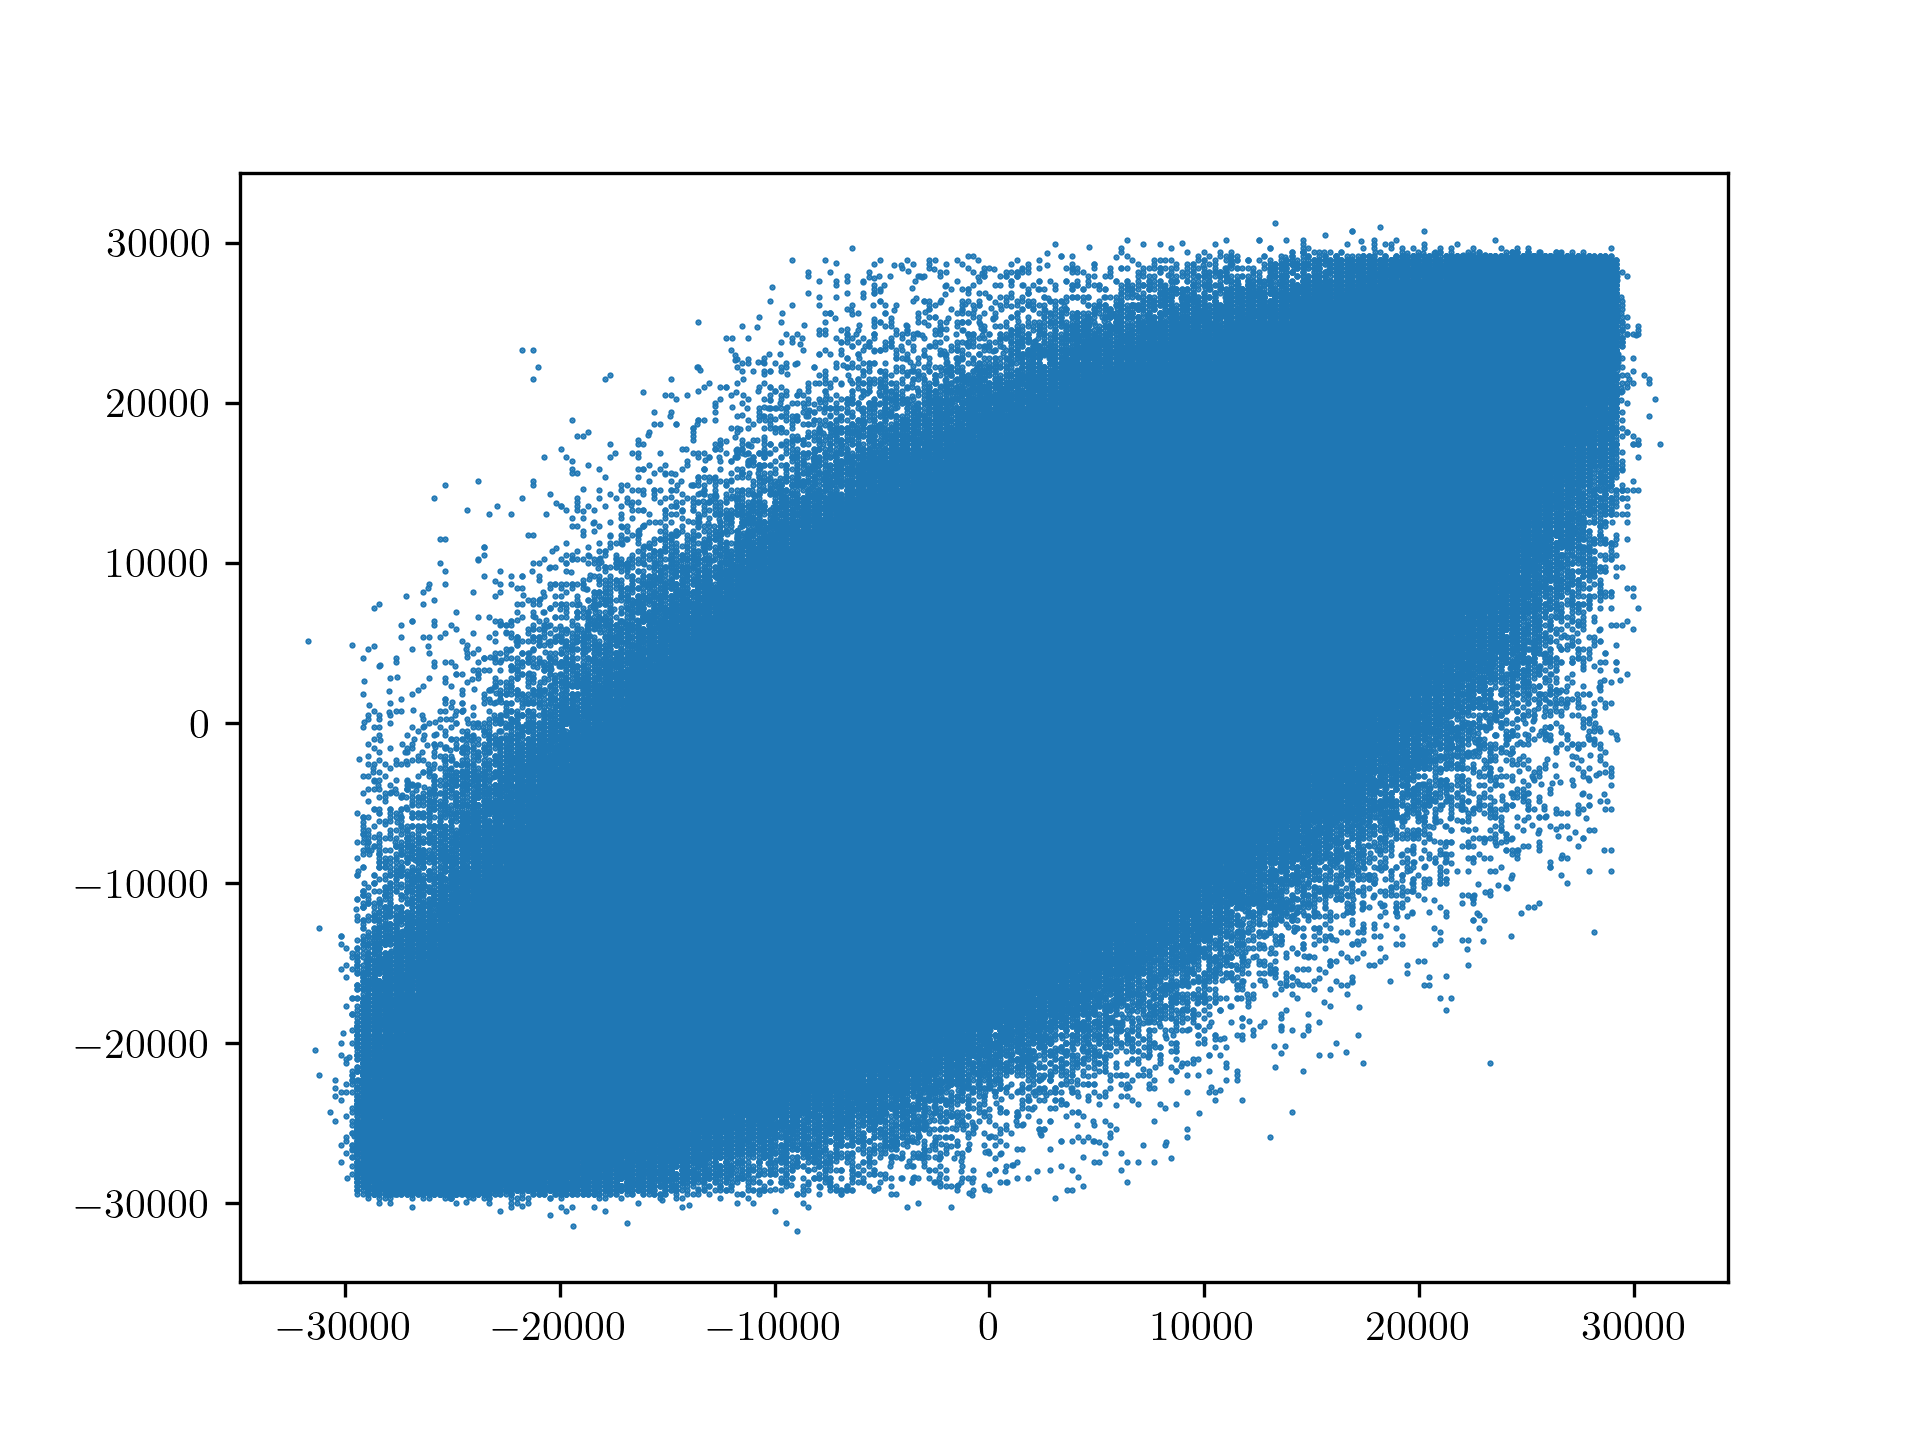
\includegraphics[width=\textwidth]{embedded1Correlation.png}
            \caption{Original}
            \label{fig:embedded1Correlation}
        \end{center}
    \end{subfigure}
    \begin{subfigure}[h]{0.3\textwidth}
        \begin{center}
            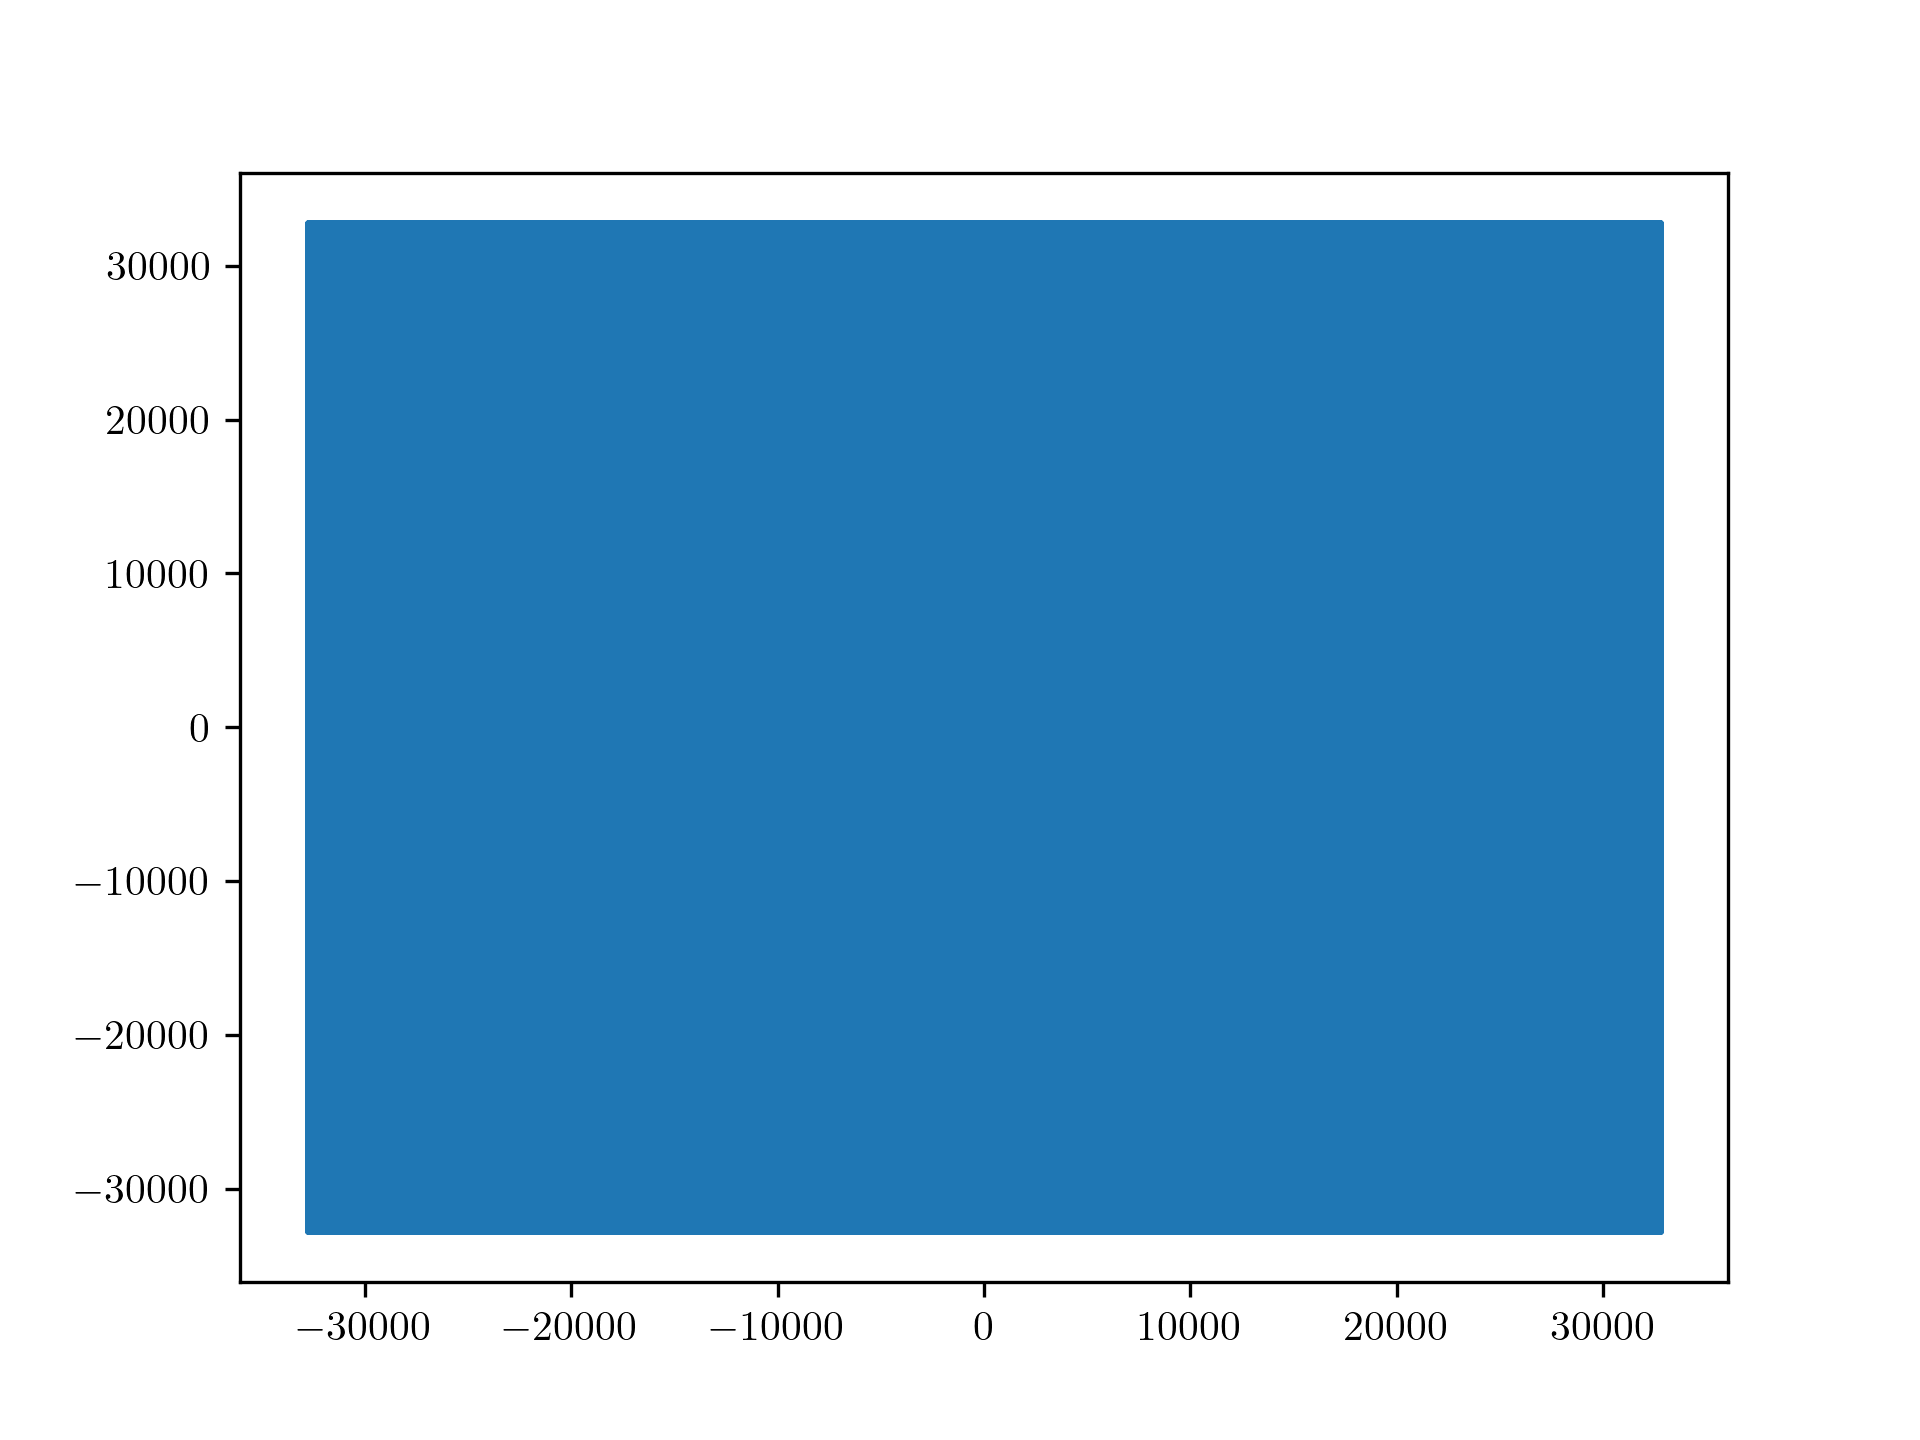
\includegraphics[width=\textwidth]{encrypted1Correlation.png}
            \caption{Encrypted}
            \label{fig:encrypted1Correlation}
        \end{center}
    \end{subfigure}
    \begin{subfigure}[h]{0.3\textwidth}
        \begin{center}
            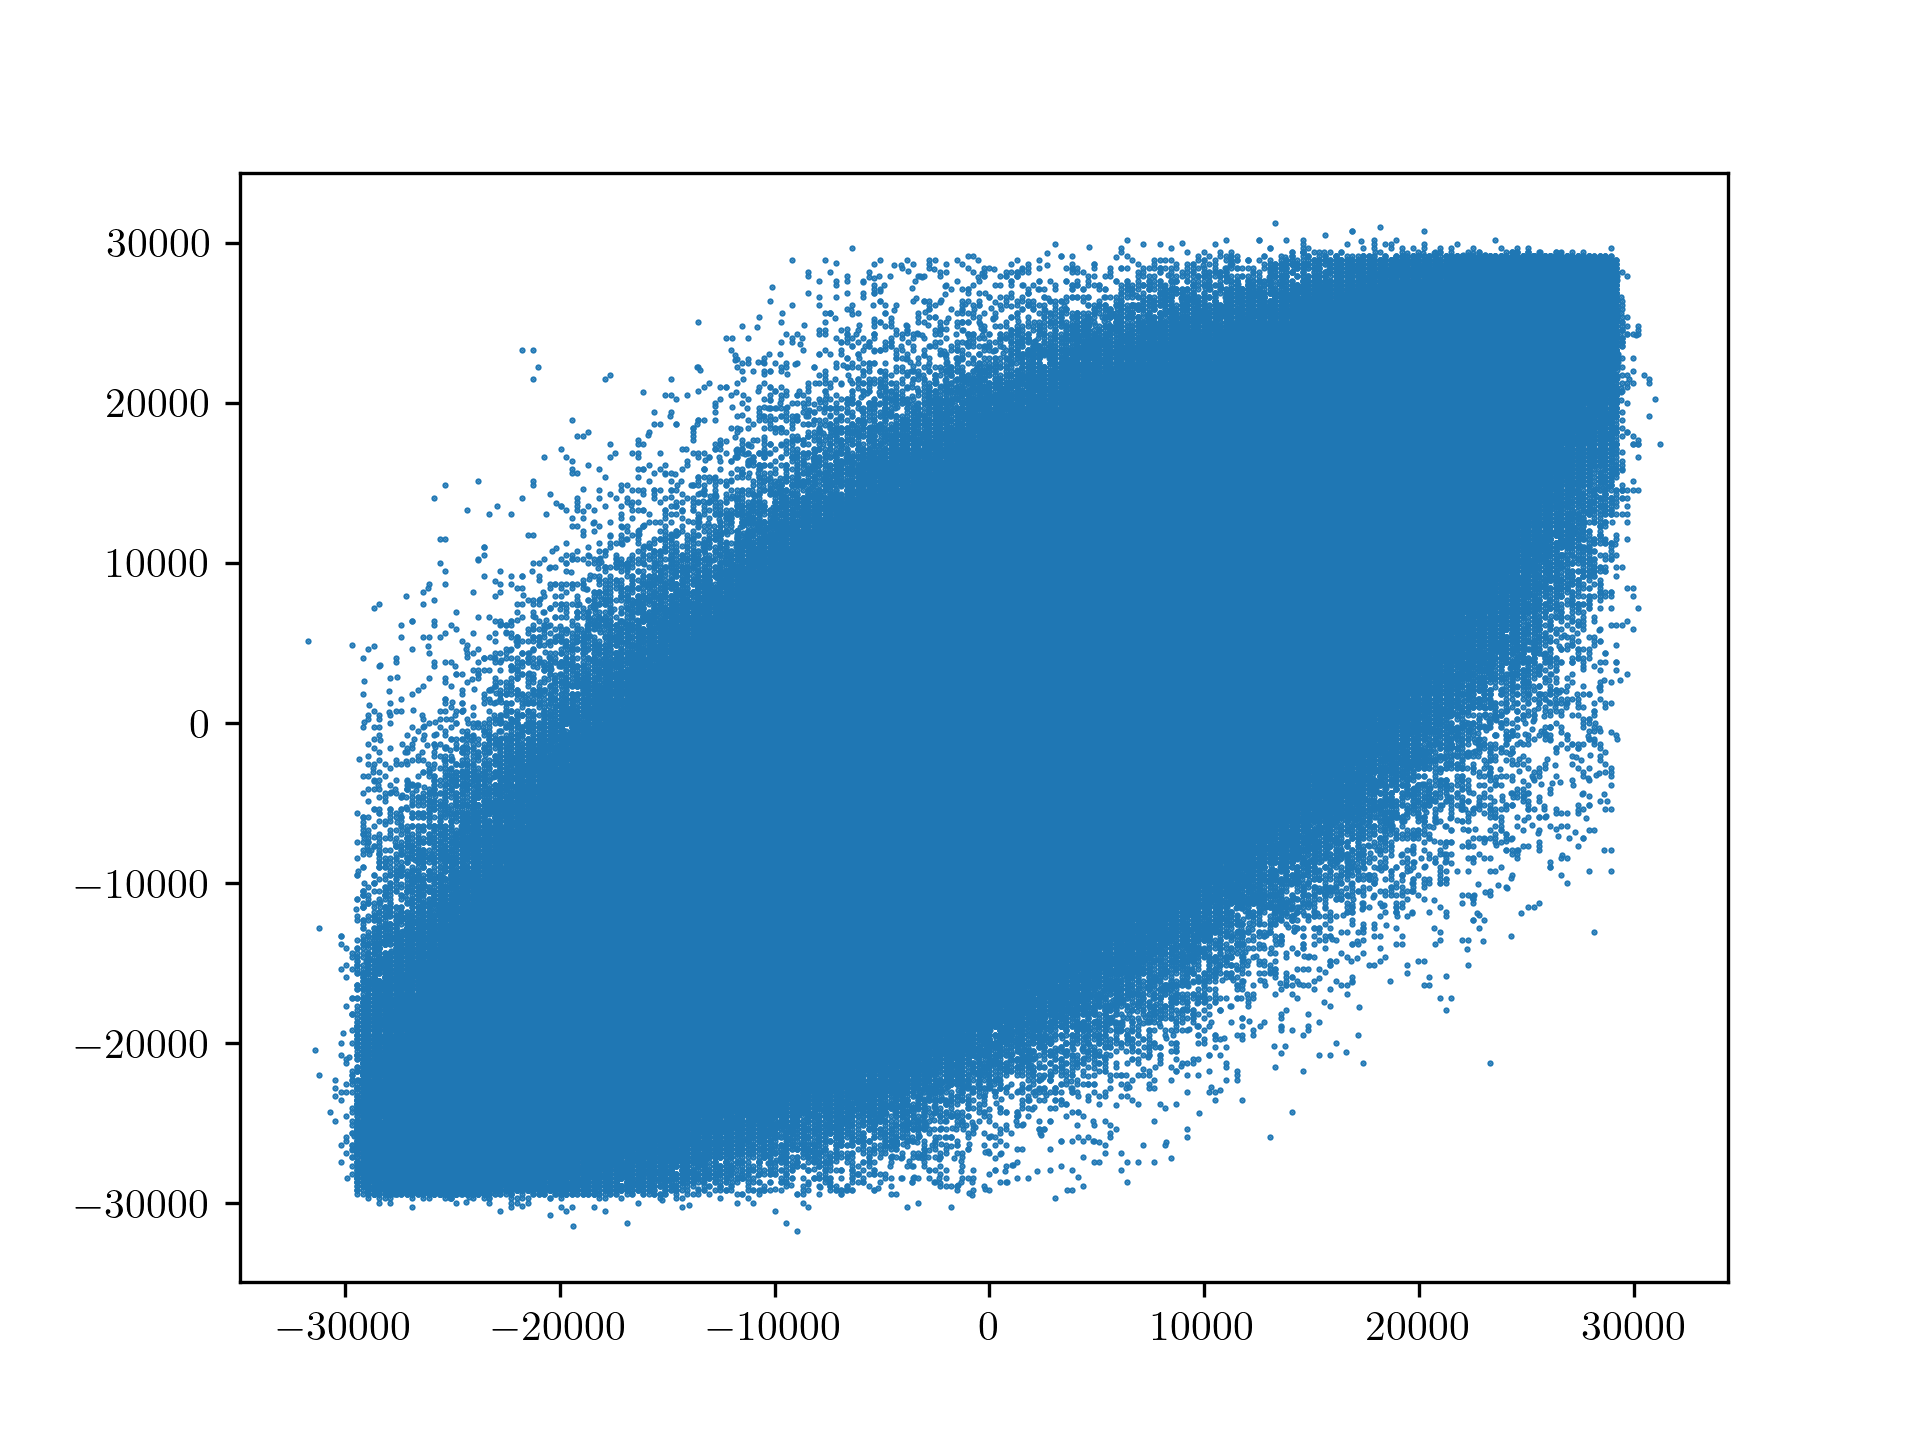
\includegraphics[width=\textwidth]{decrypted1Correlation.png}
            \caption{Decrypted}
            \label{fig:decrypted1Correlation}
        \end{center}
    \end{subfigure}
    \caption{Correlation map of Audio 1: (\ref{fig:embedded1Correlation}) before encryption, (\ref{fig:encrypted1Correlation}) after encryption and (\ref{fig:decrypted1Correlation}) after decryption.}
    \label{fig:audio1Correlation}
\end{figure}
\begin{figure}[pos=h]
    \begin{subfigure}[h]{0.3\textwidth}
        \begin{center}
            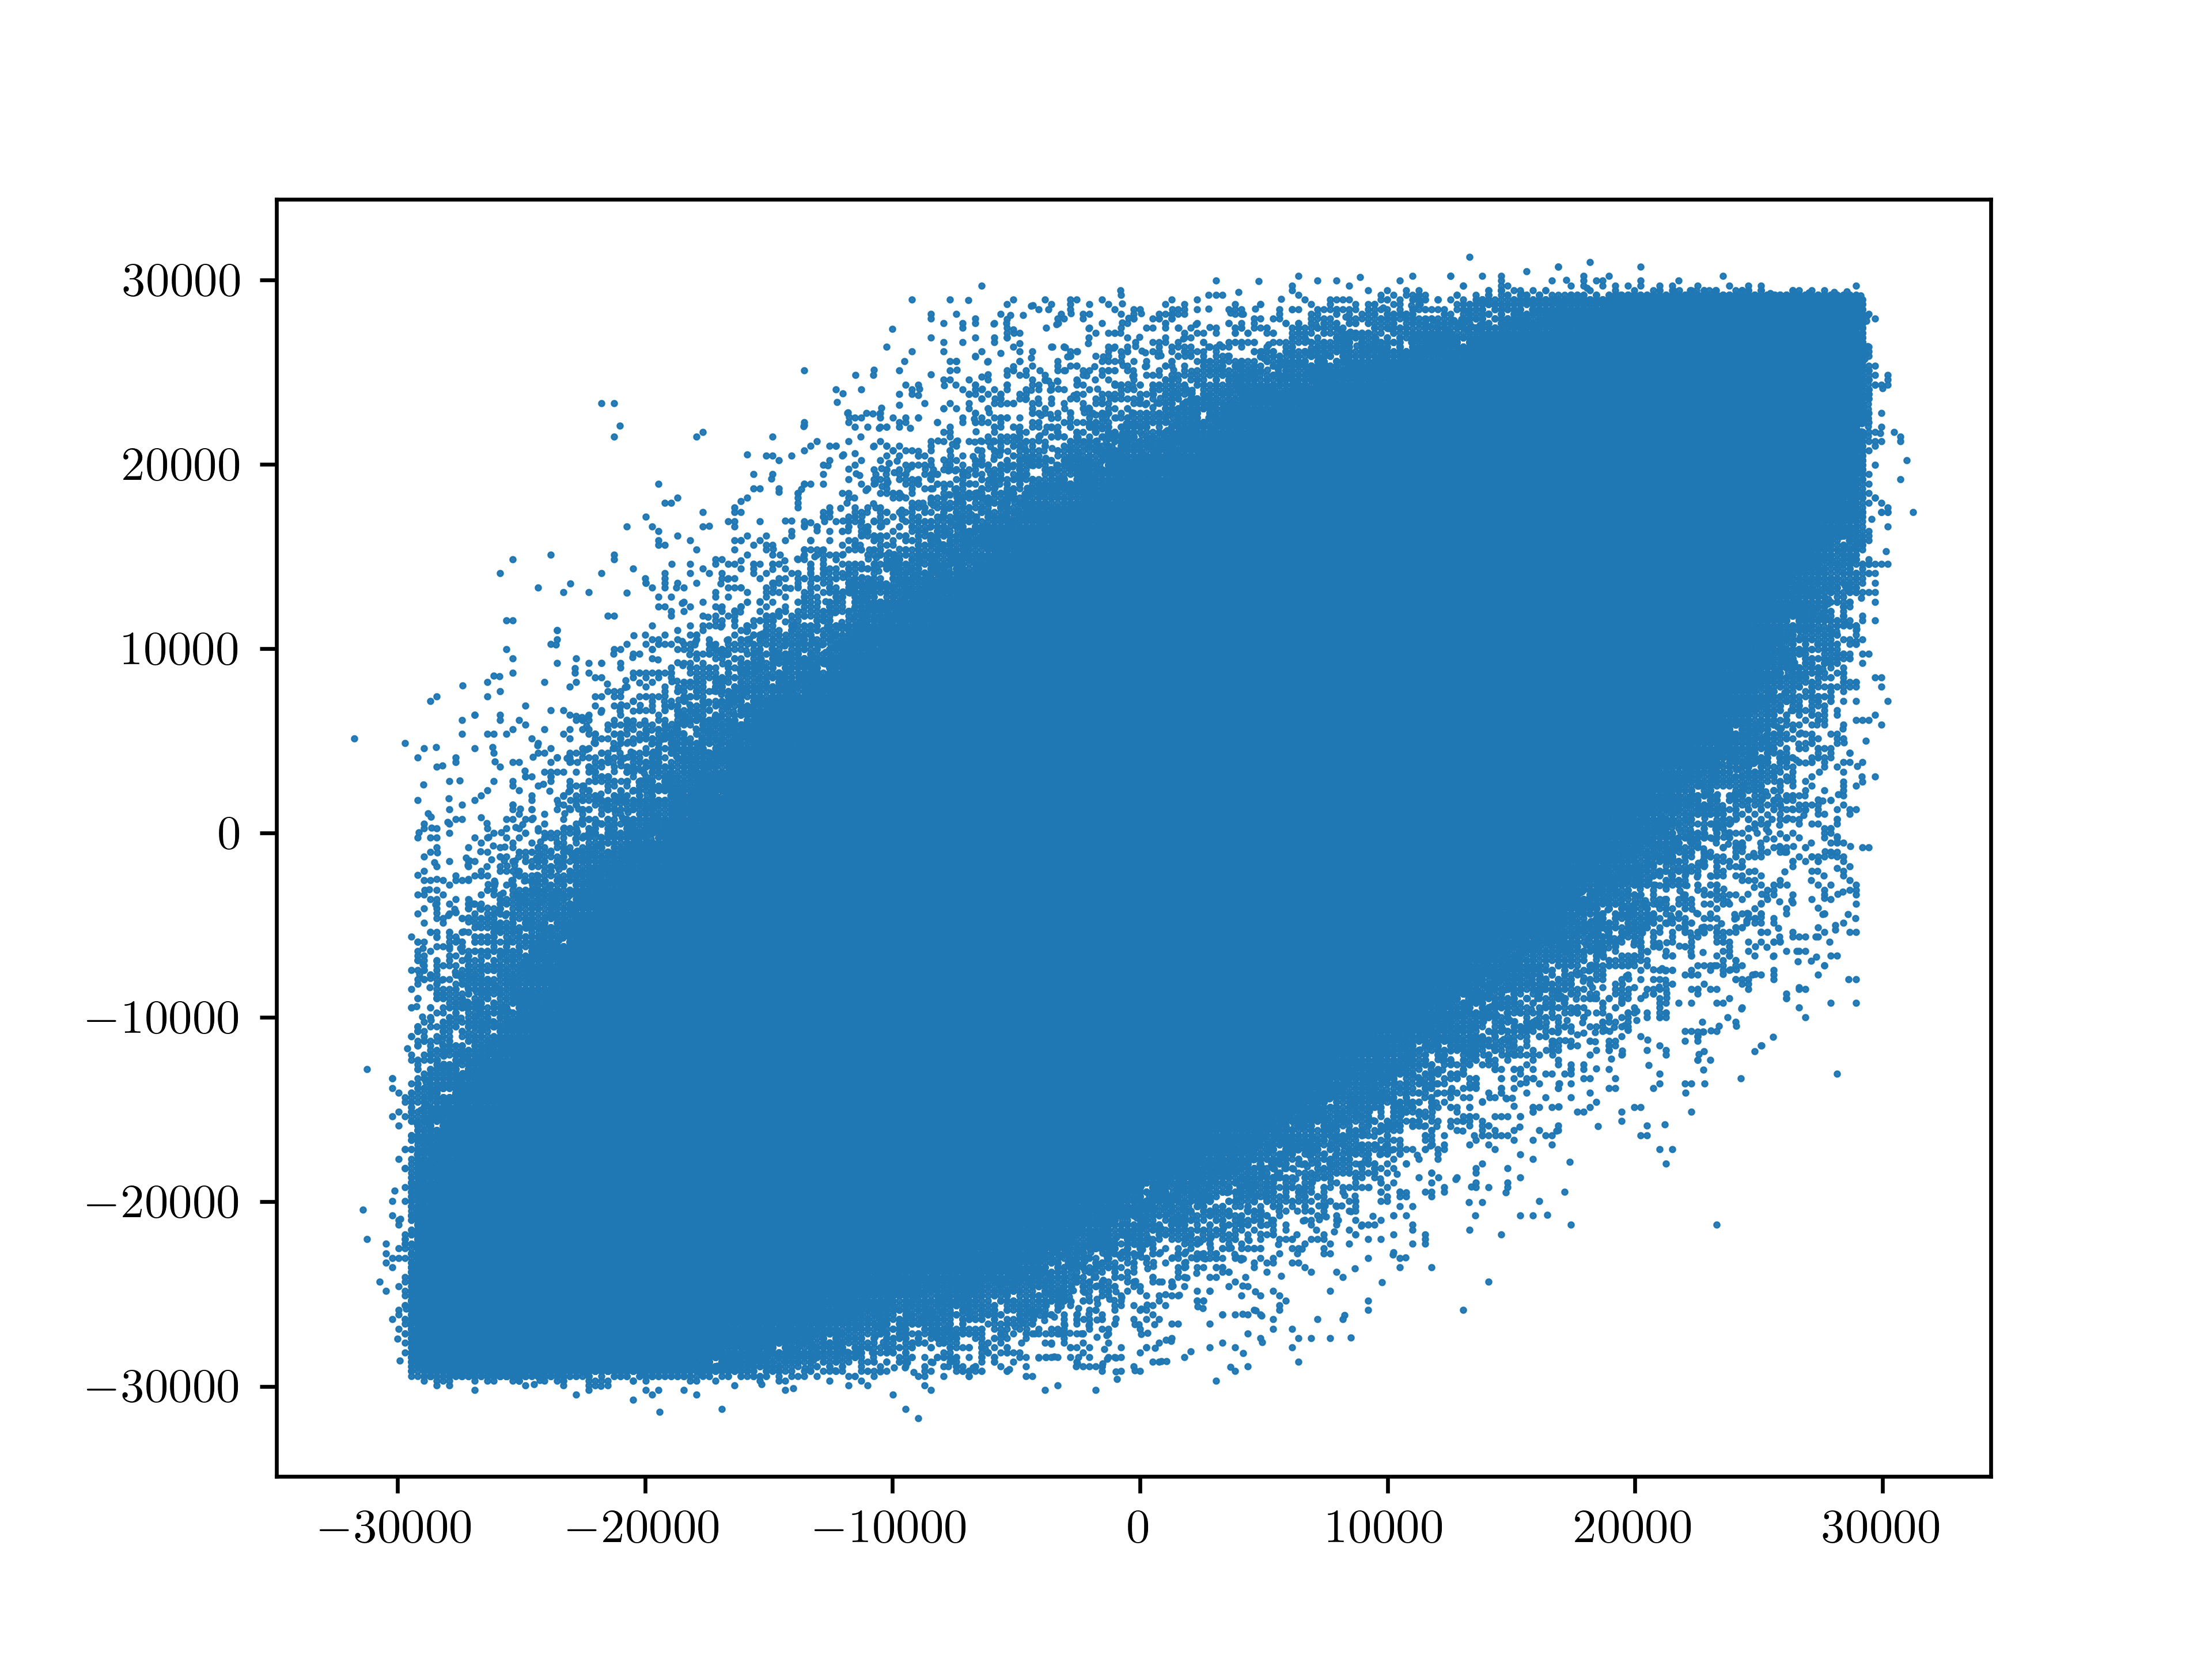
\includegraphics[width=\textwidth]{embedded2Correlation.png}
            \caption{Original}
            \label{fig:embedded2Correlation}
        \end{center}
    \end{subfigure}
    \begin{subfigure}[h]{0.3\textwidth}
        \begin{center}
            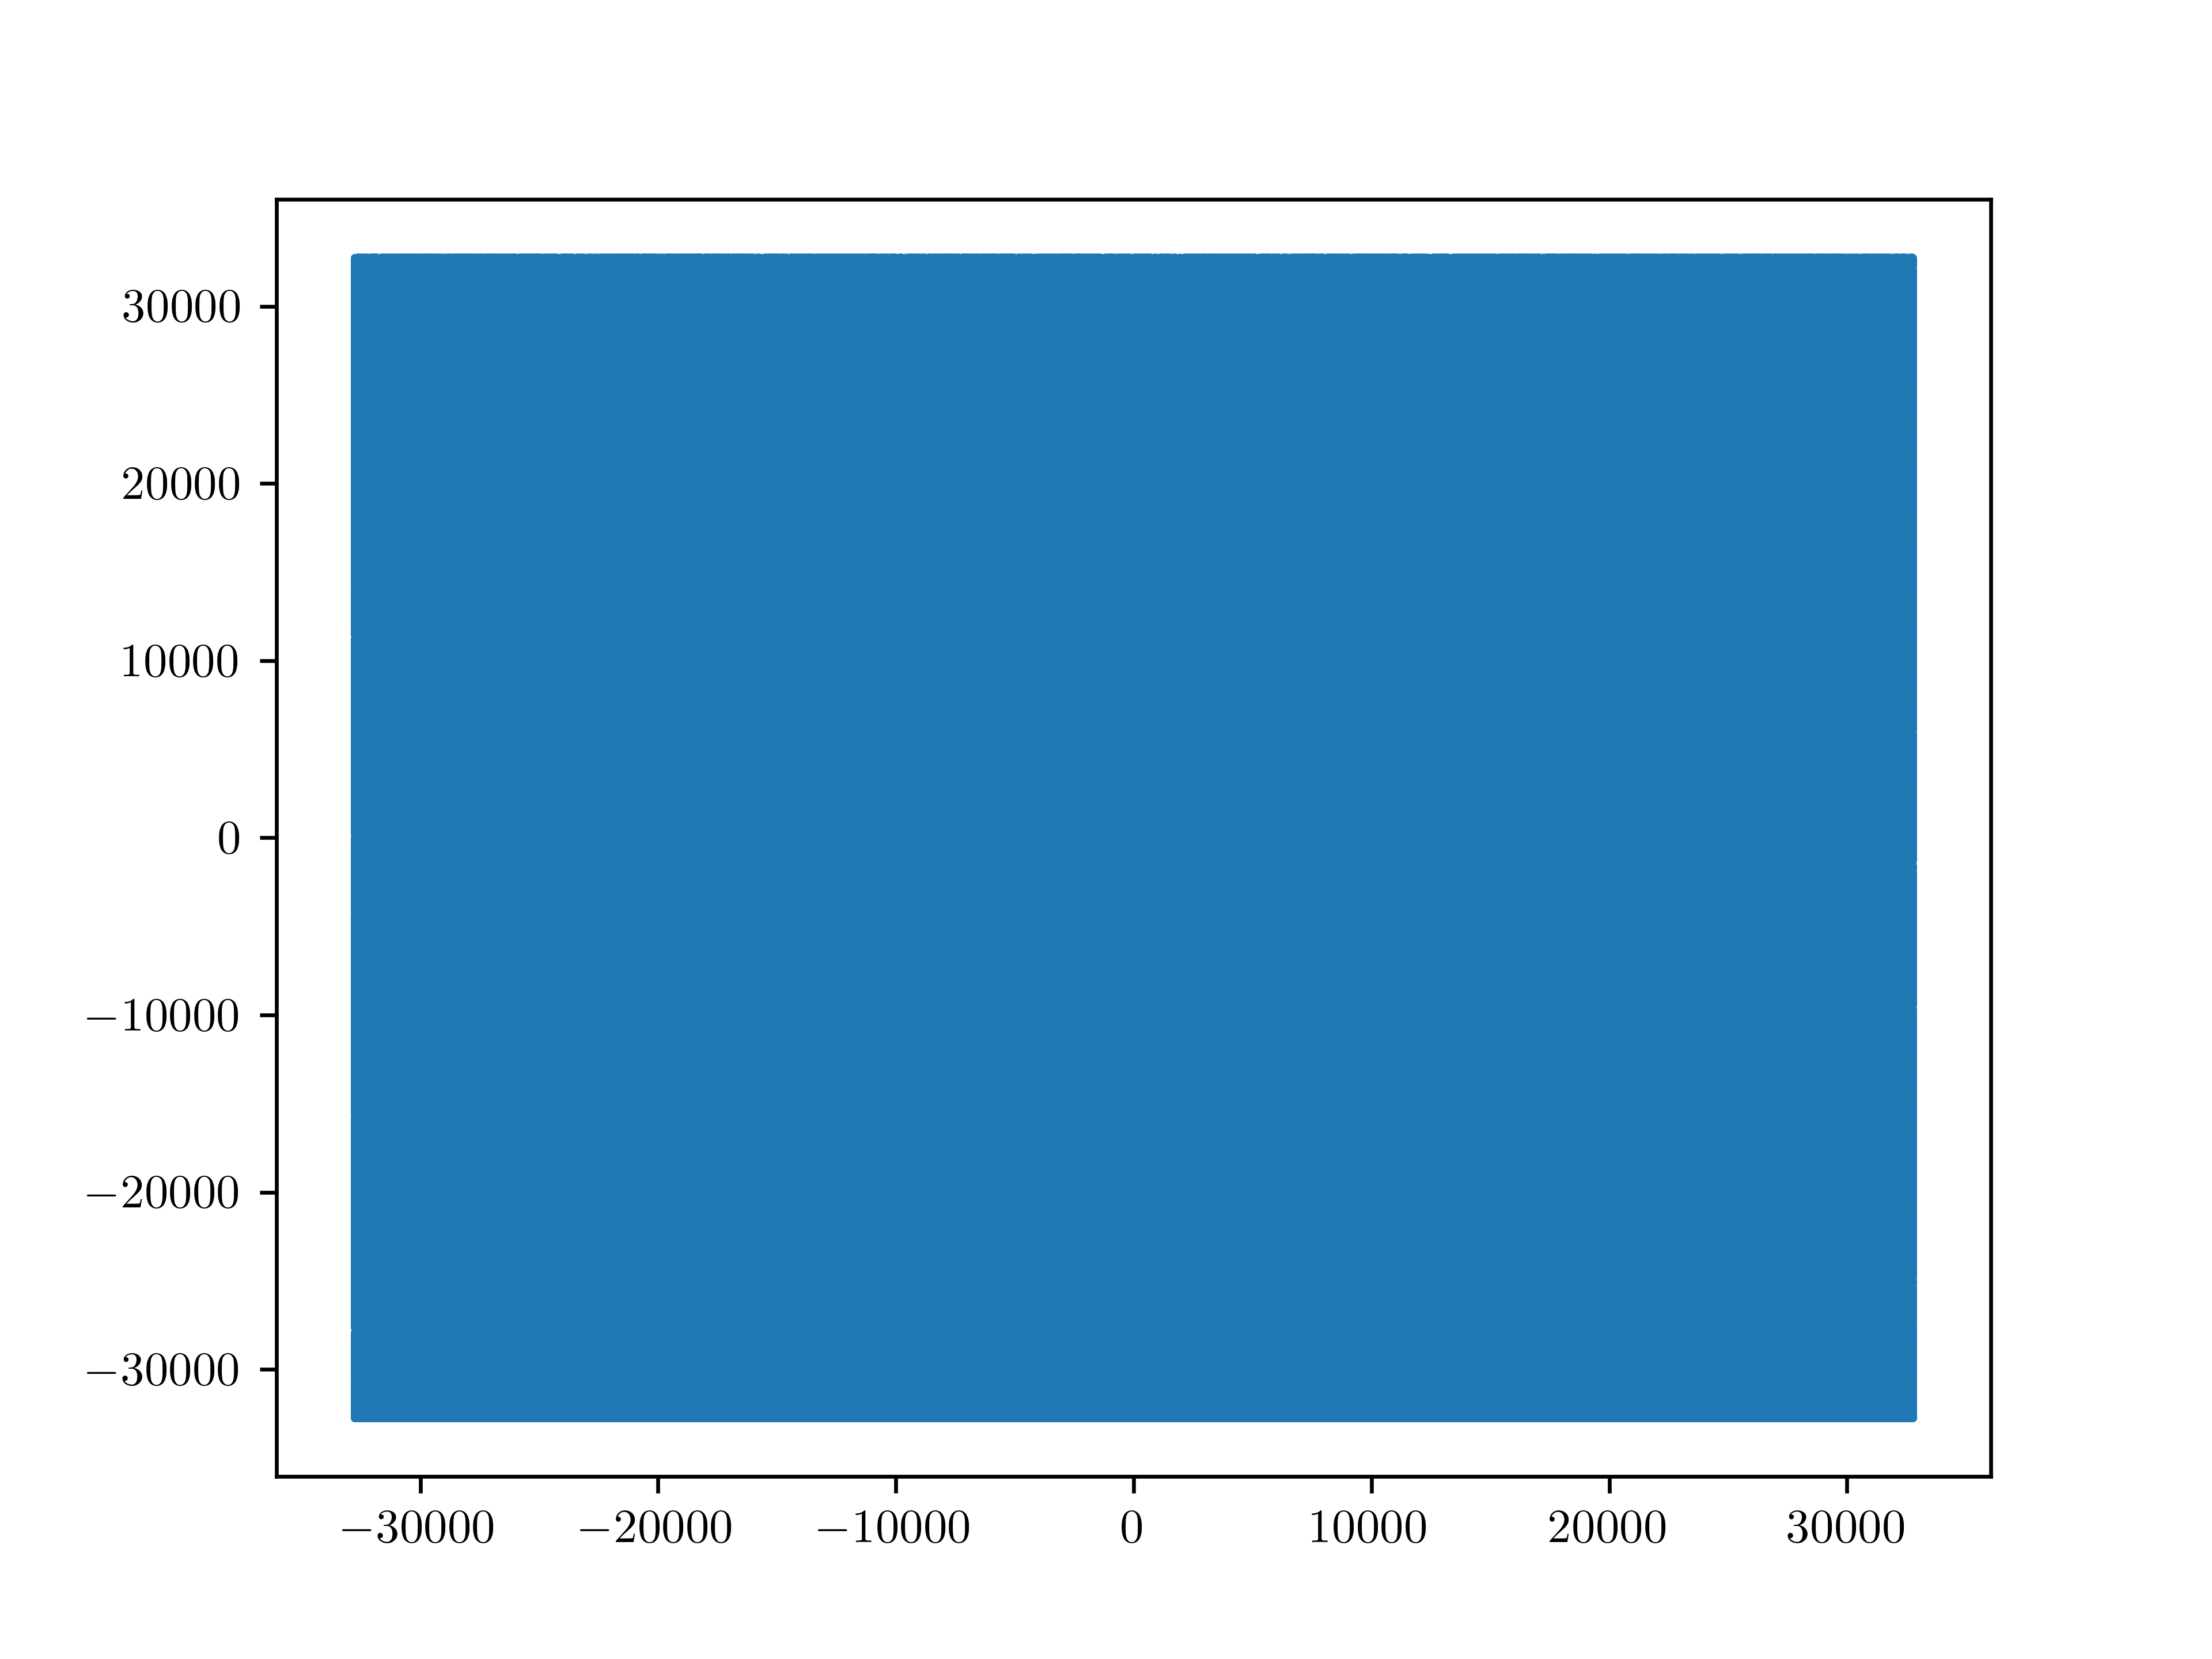
\includegraphics[width=\textwidth]{encrypted2Correlation.png}
            \caption{Encrypted}
            \label{fig:encrypted2Correlation}
        \end{center}
    \end{subfigure}
    \begin{subfigure}[h]{0.3\textwidth}
        \begin{center}
            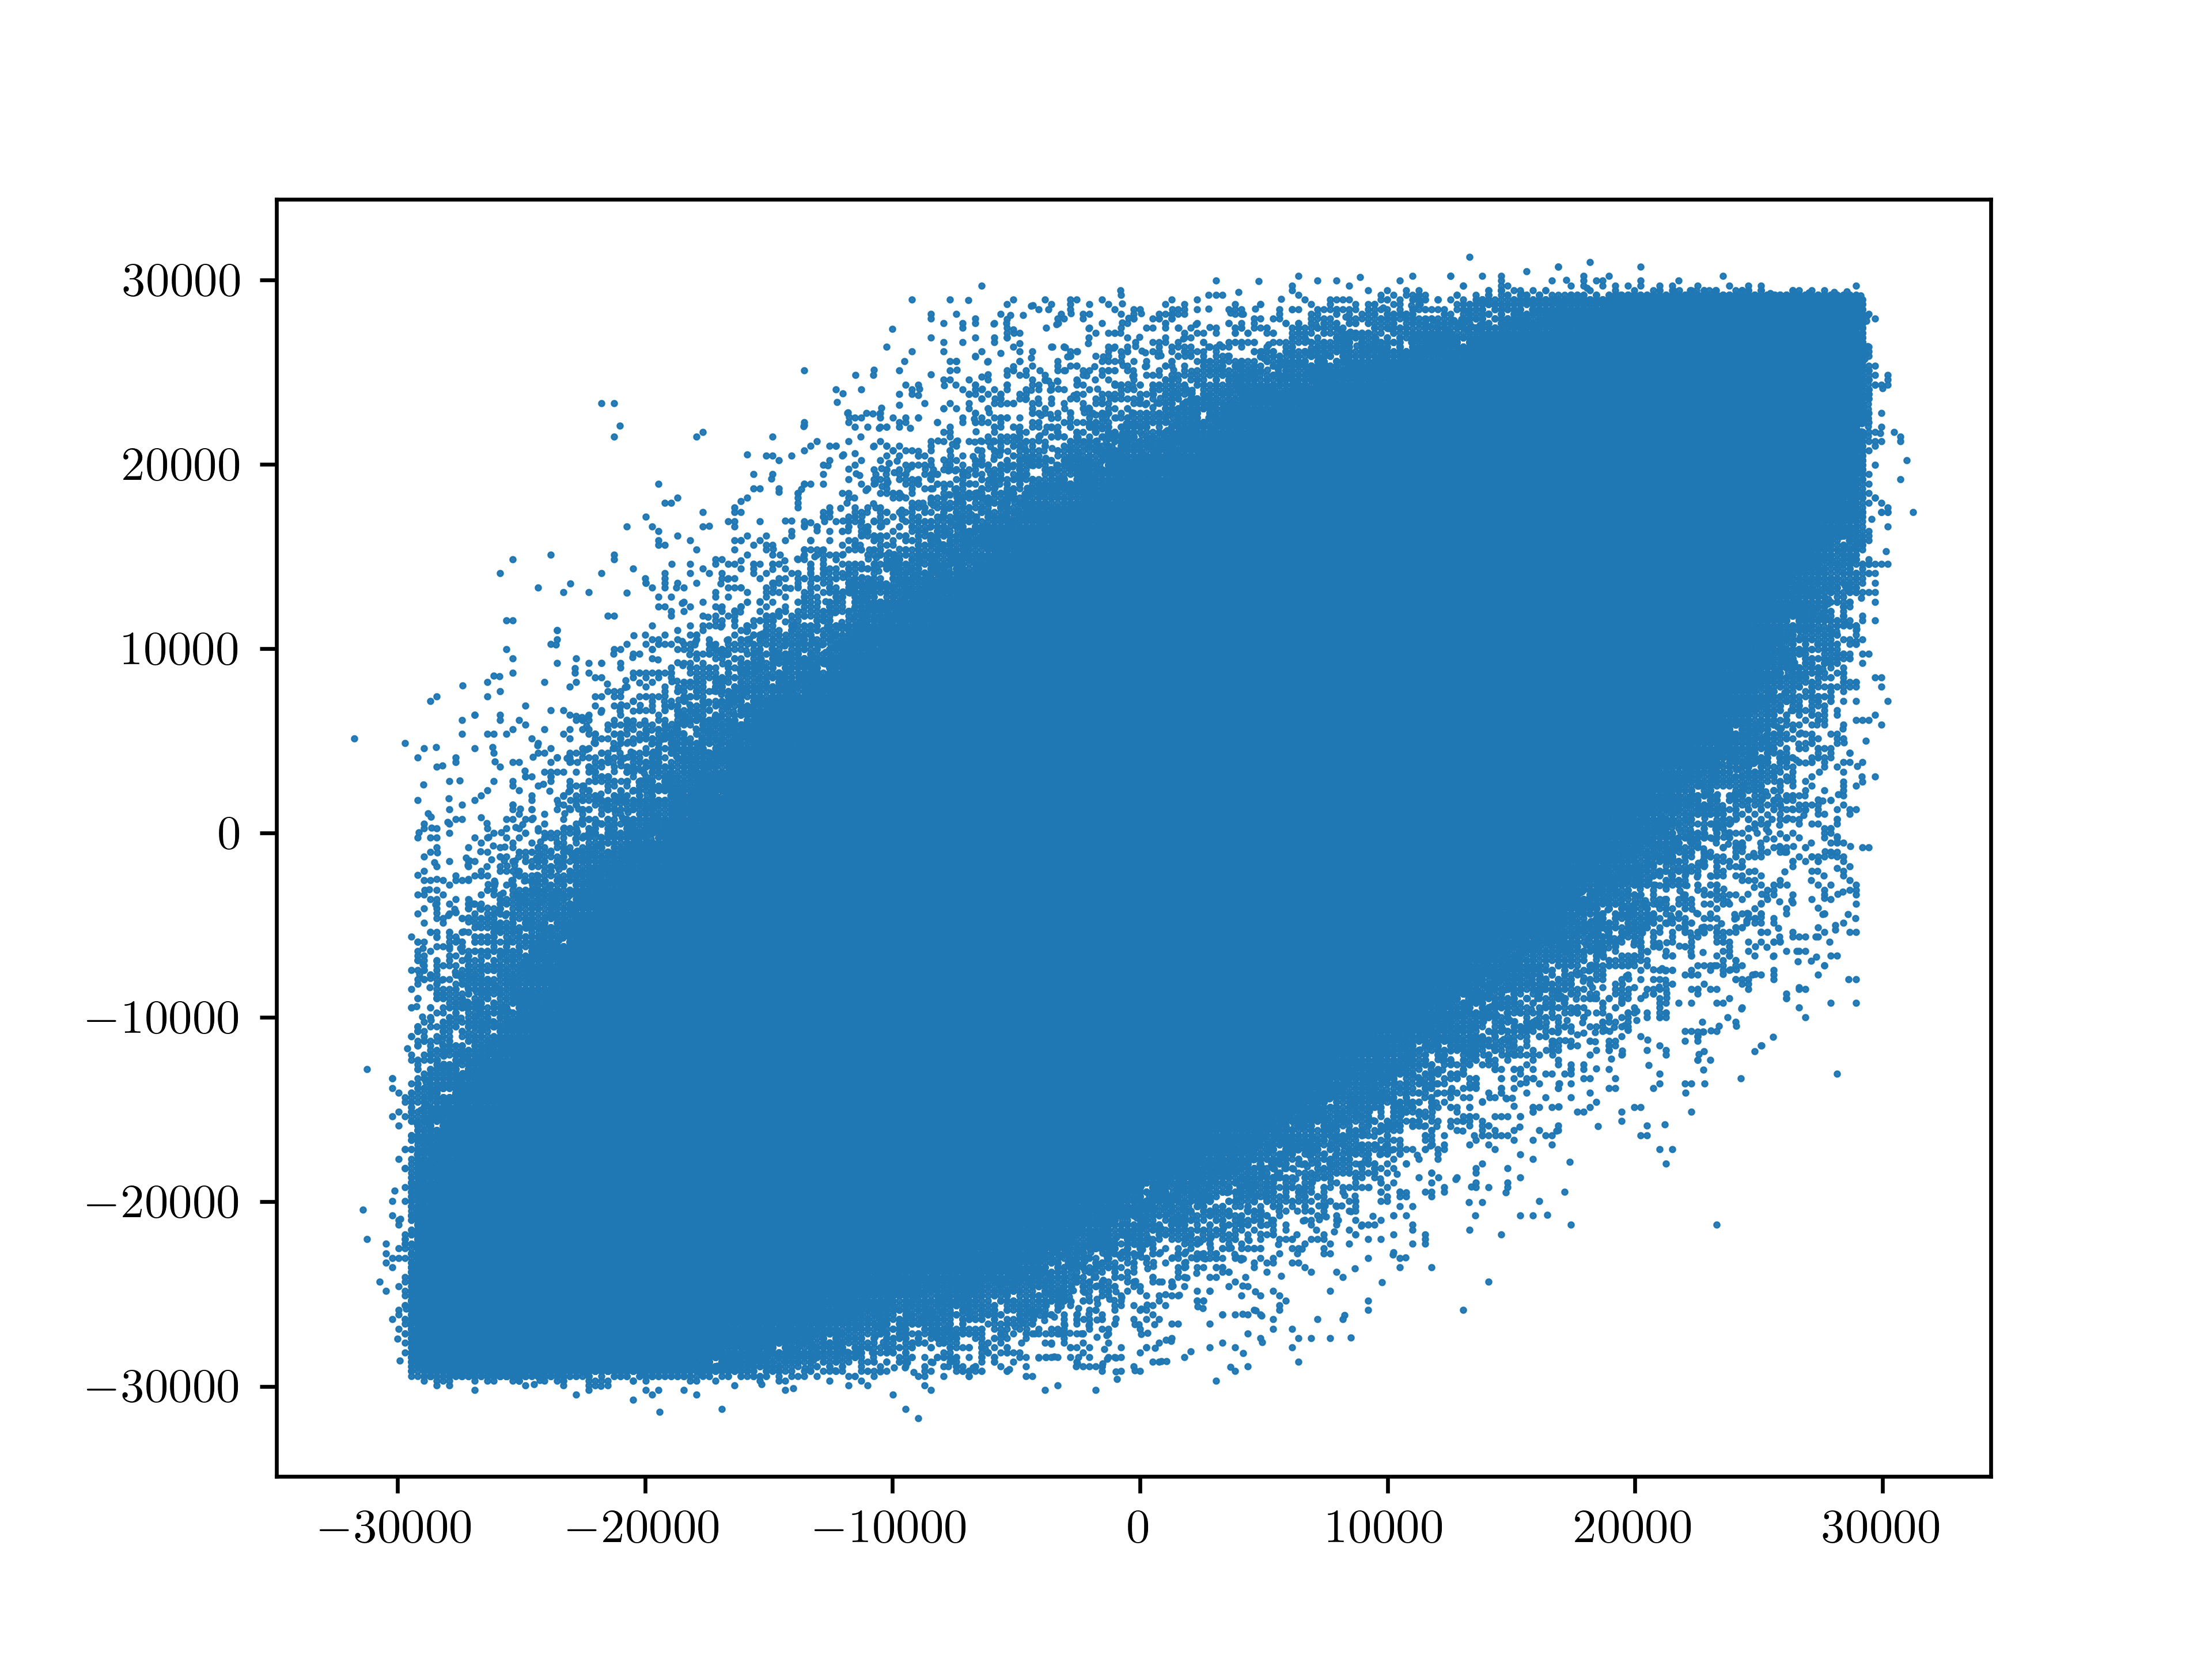
\includegraphics[width=\textwidth]{decrypted2Correlation.png}
            \caption{Decrypted}
            \label{fig:decrypted2Correlation}
        \end{center}
    \end{subfigure}
    \caption{Correlation map of Audio 2: (\ref{fig:embedded2Correlation}) before encryption, (\ref{fig:encrypted2Correlation}) after encryption and (\ref{fig:decrypted2Correlation}) after decryption.}
    \label{fig:audio2Correlation}
\end{figure}
\subsubsection{Histogram Analysis}
Histogram is a visual representation of how data is distributed. For audio signals, Histogram depicts the sample frequency with respect to sample amplitude. For a good encryption, the histogram is expected to be uniformly distributed instead of being converging or diverging. Figure \ref{fig:audio1Histogram} and \ref{fig:audio2Histogram} shows the histogram before encryption, after encryption and after encryption of Audio 1 and Audio 2 produced through steganography, respectively.
\begin{figure}[pos=h]
    \begin{subfigure}[h]{0.3\textwidth}
        \begin{center}
            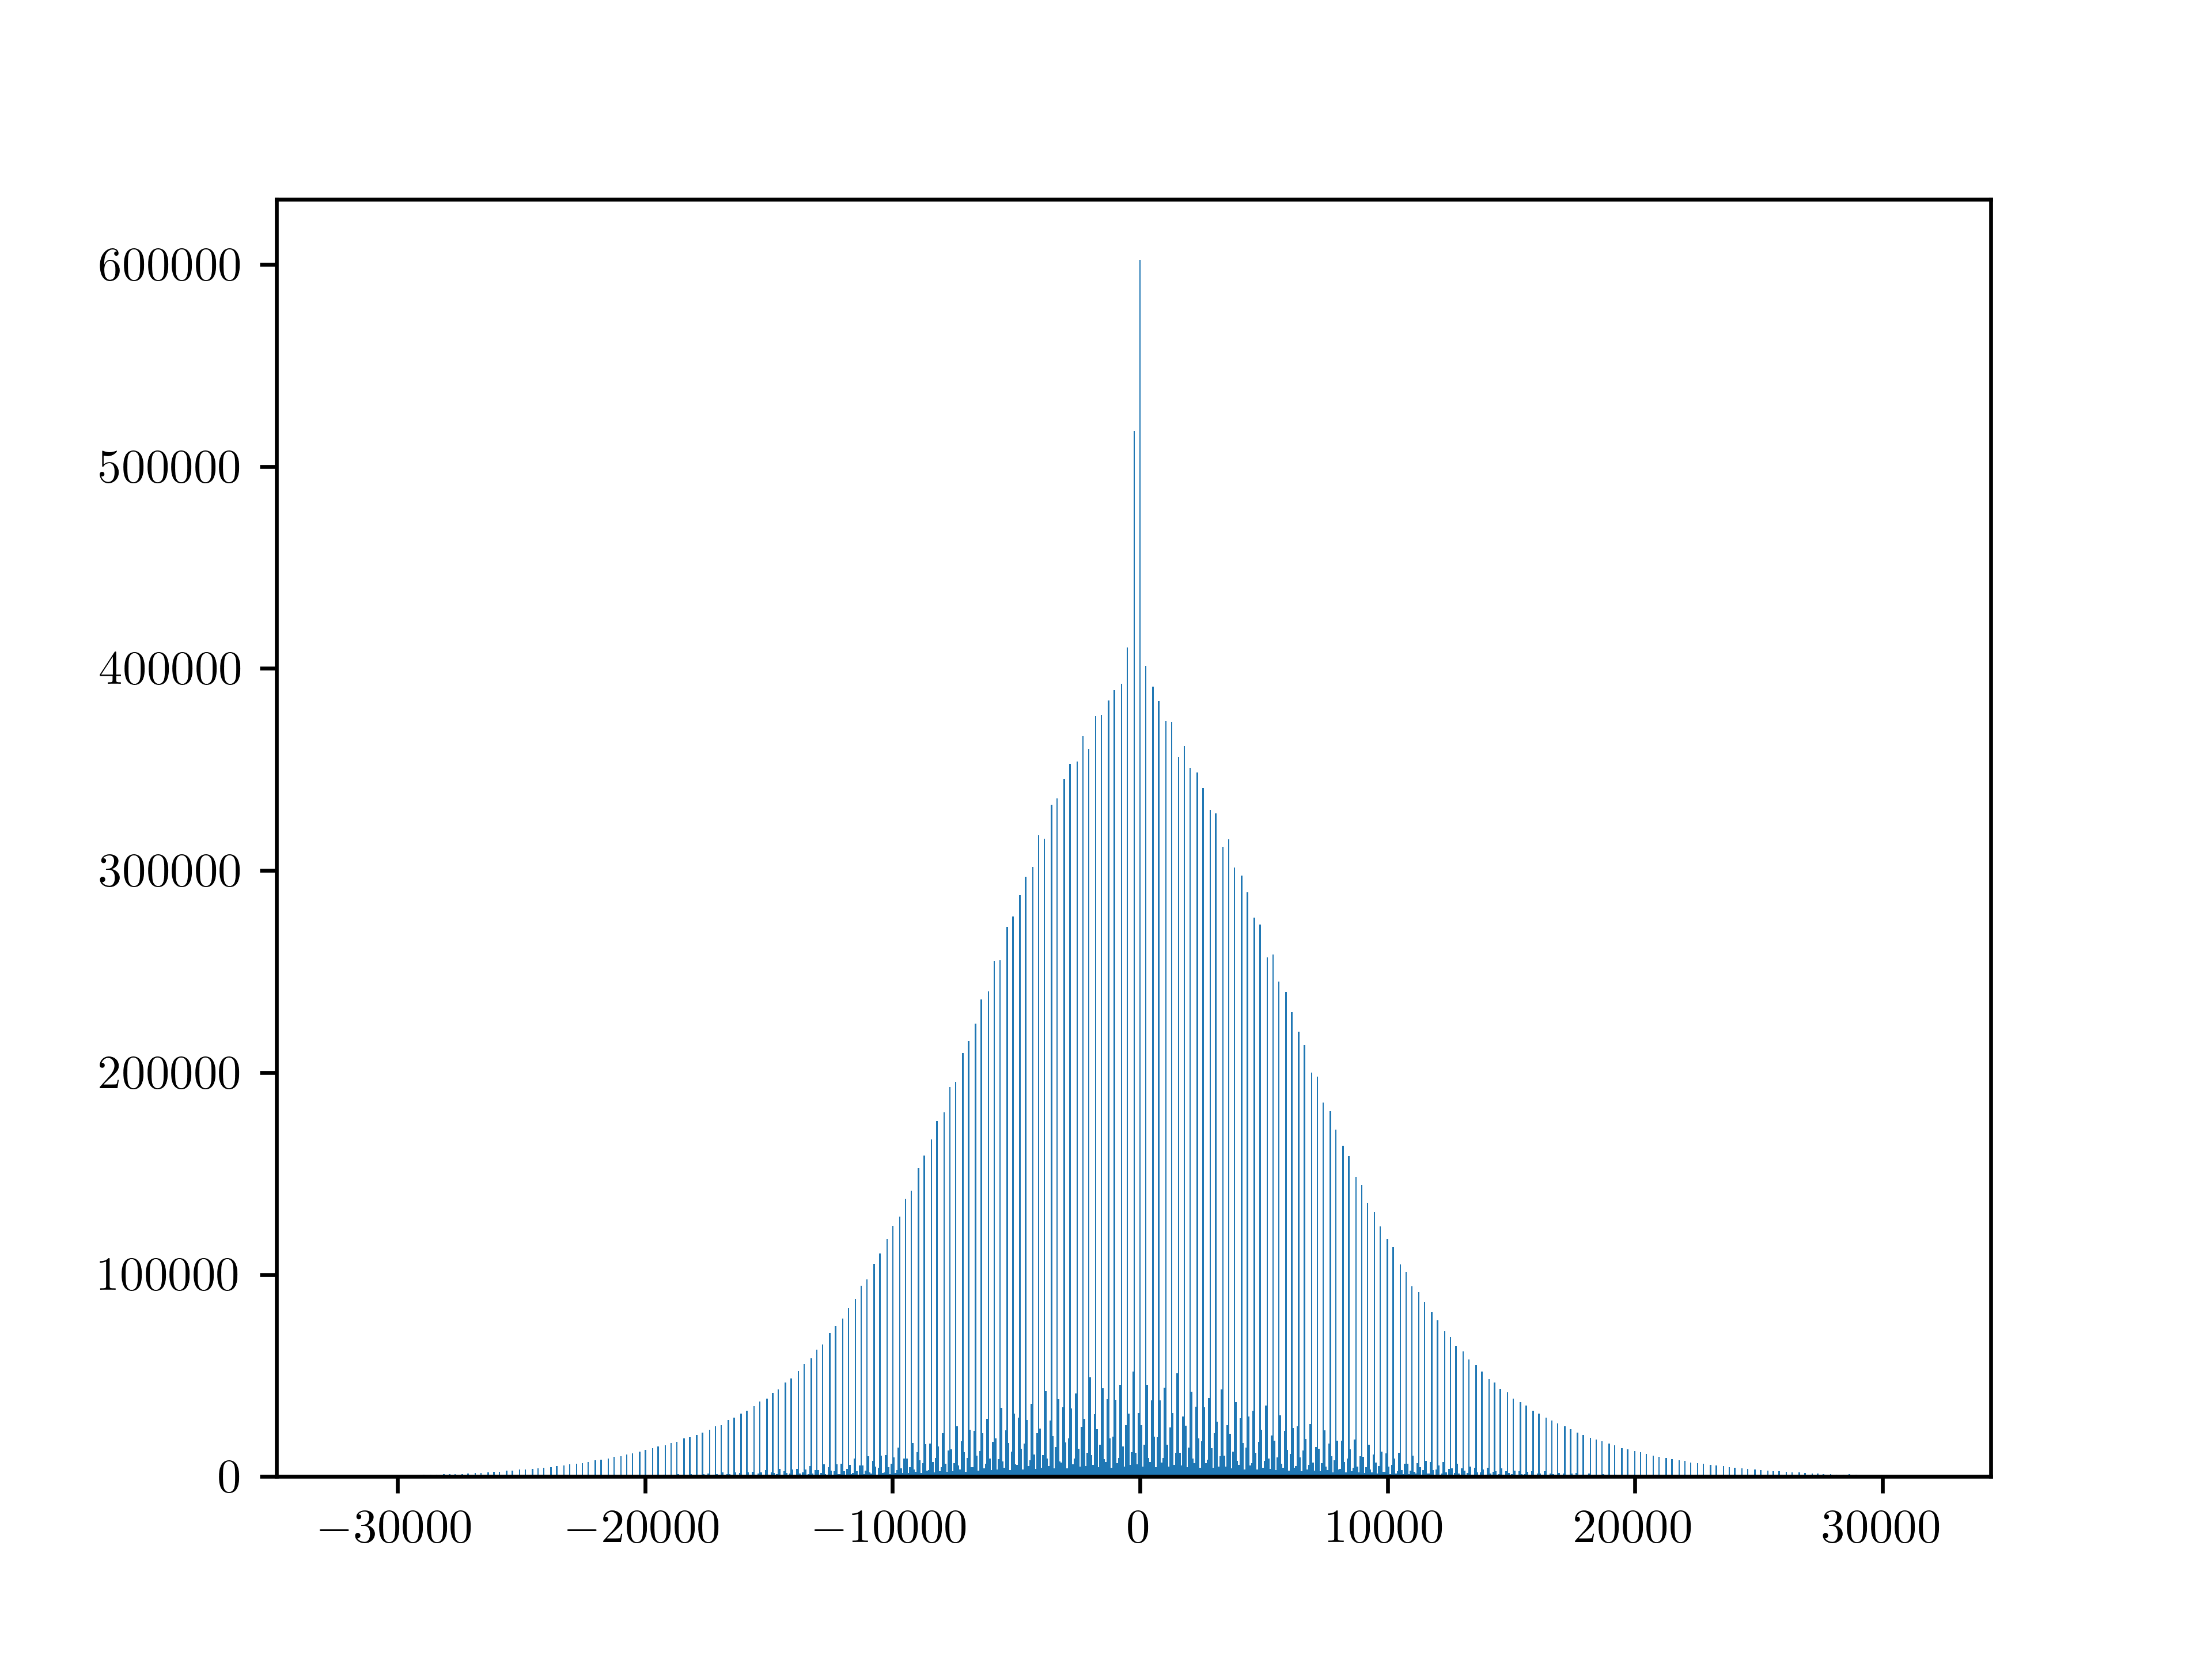
\includegraphics[width=\textwidth]{embedded1Histogram.png}
            \caption{Original}
            \label{fig:embedded1Histogram}
        \end{center}
    \end{subfigure}
    \begin{subfigure}[h]{0.3\textwidth}
        \begin{center}
            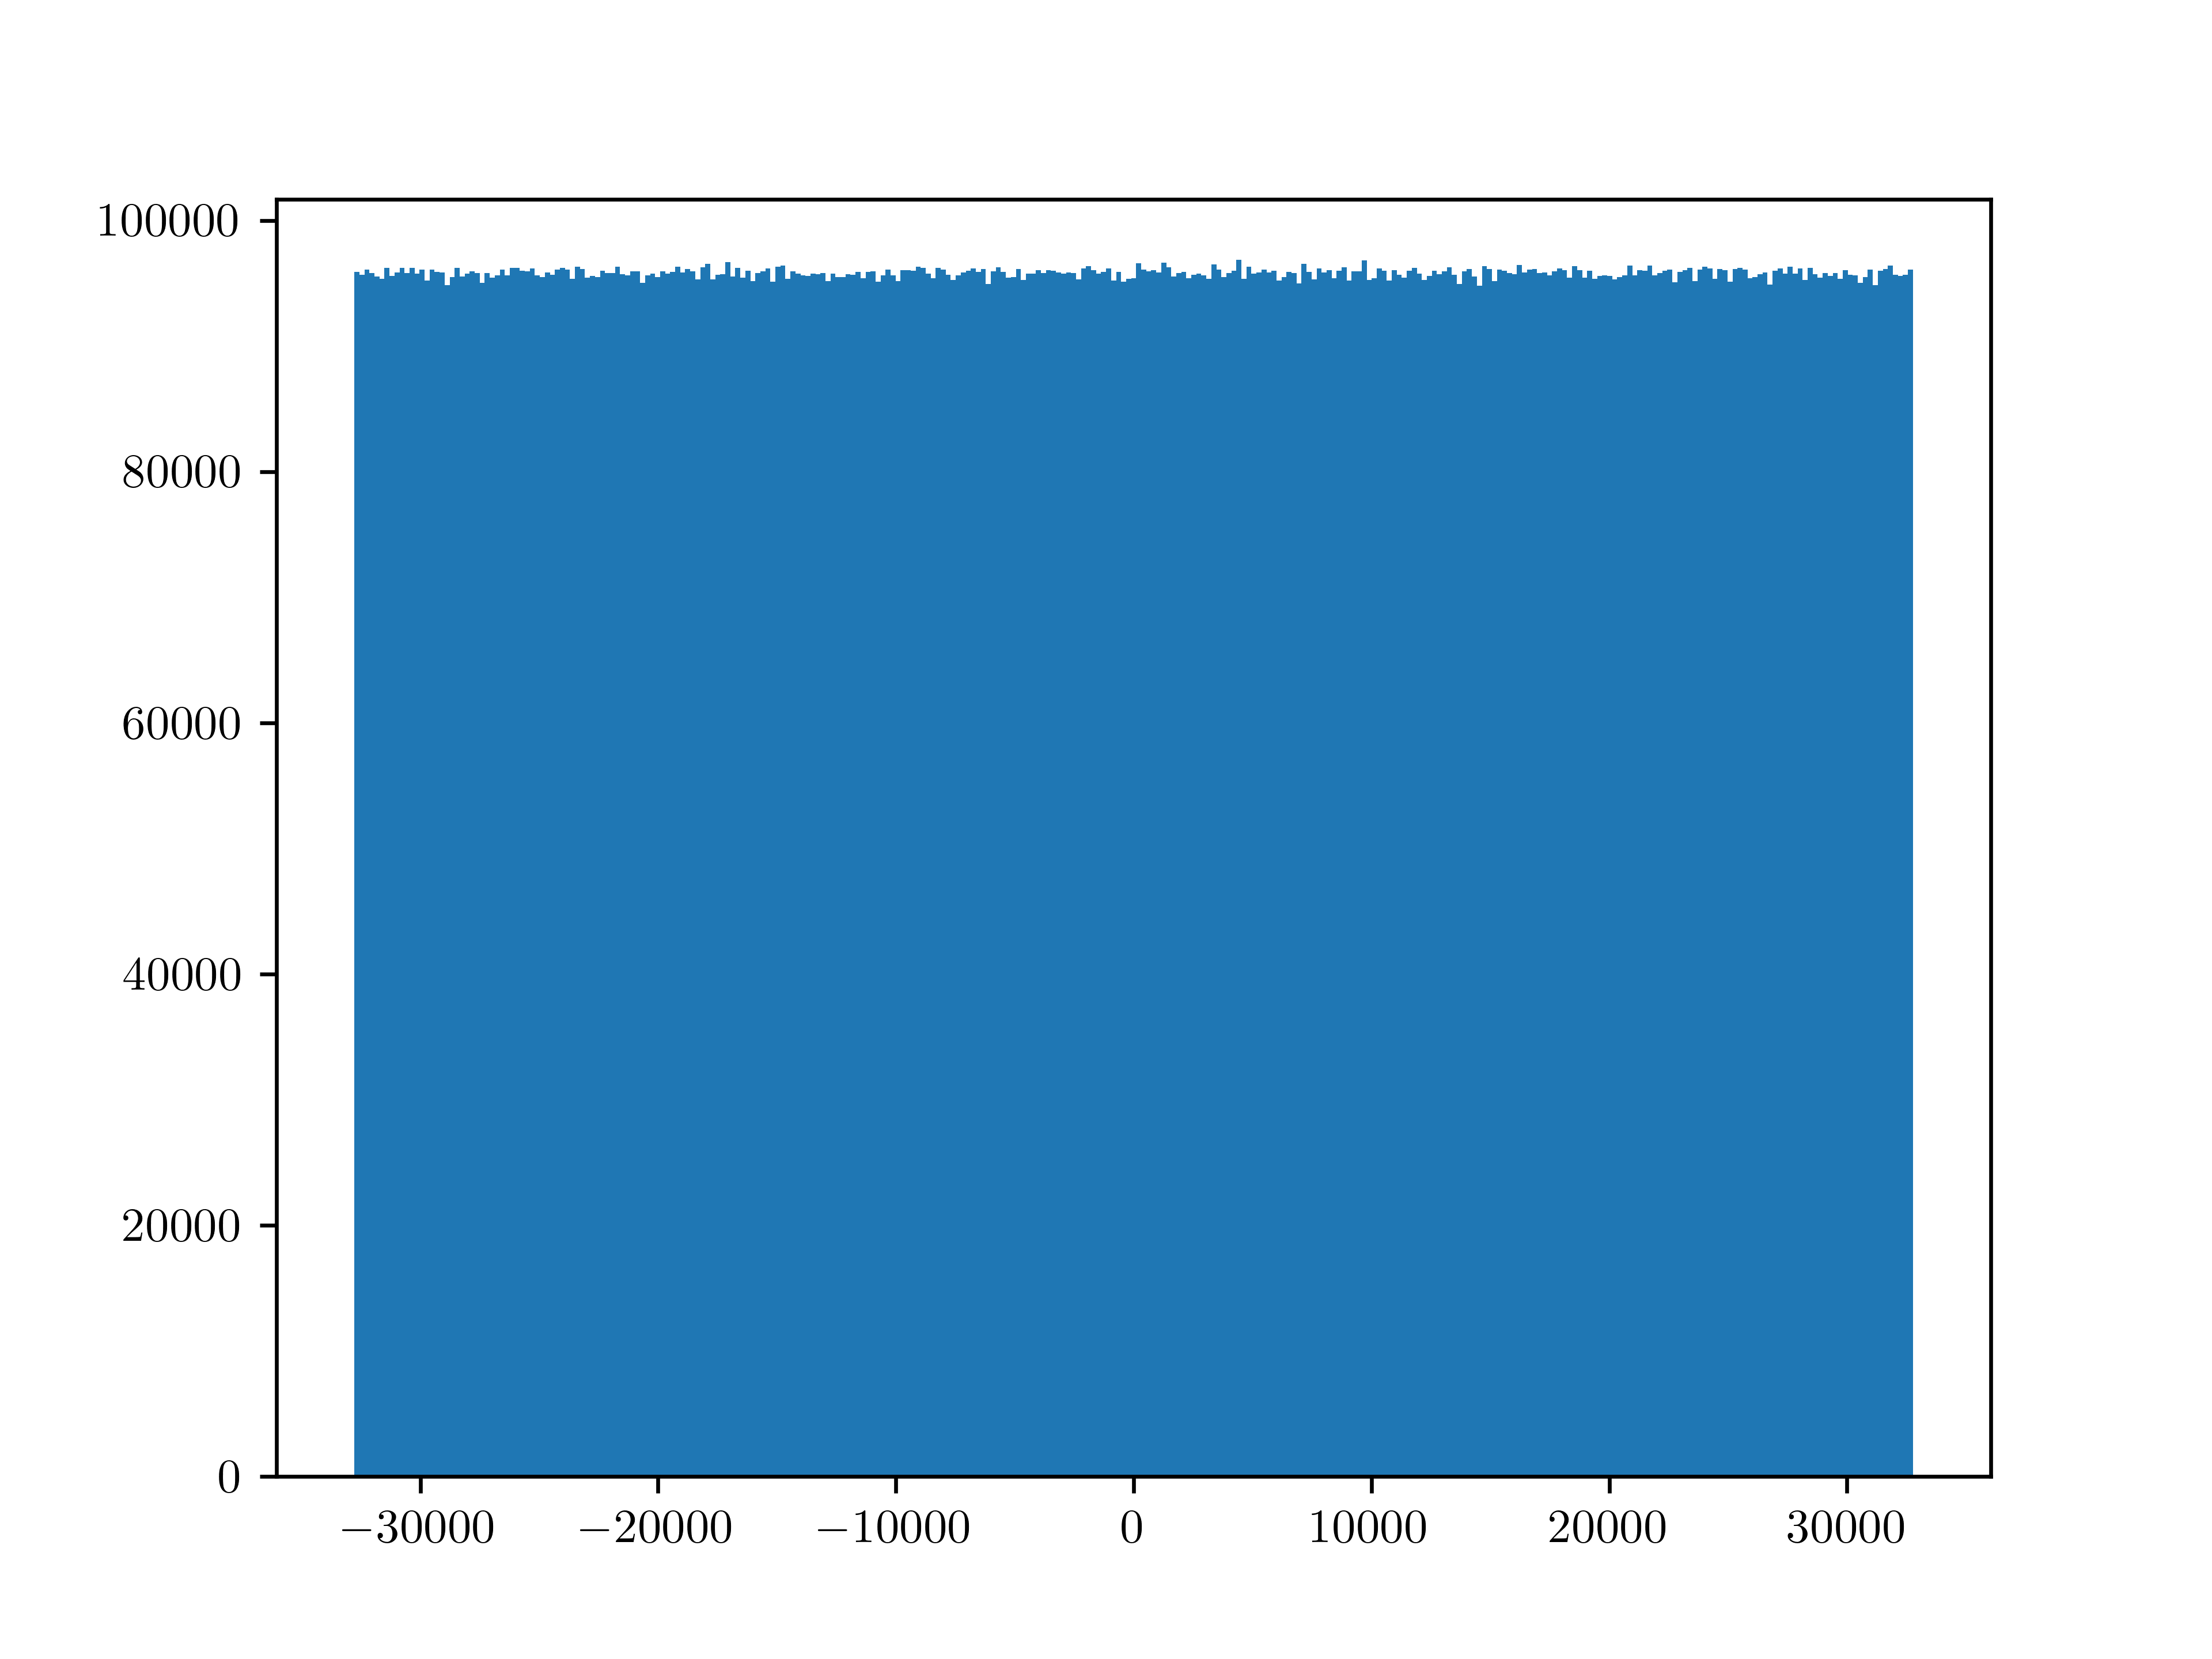
\includegraphics[width=\textwidth]{encrypted1Histogram.png}
            \caption{Encrypted}
            \label{fig:encrypted1Histogram}
        \end{center}
    \end{subfigure}
    \begin{subfigure}[h]{0.3\textwidth}
        \begin{center}
            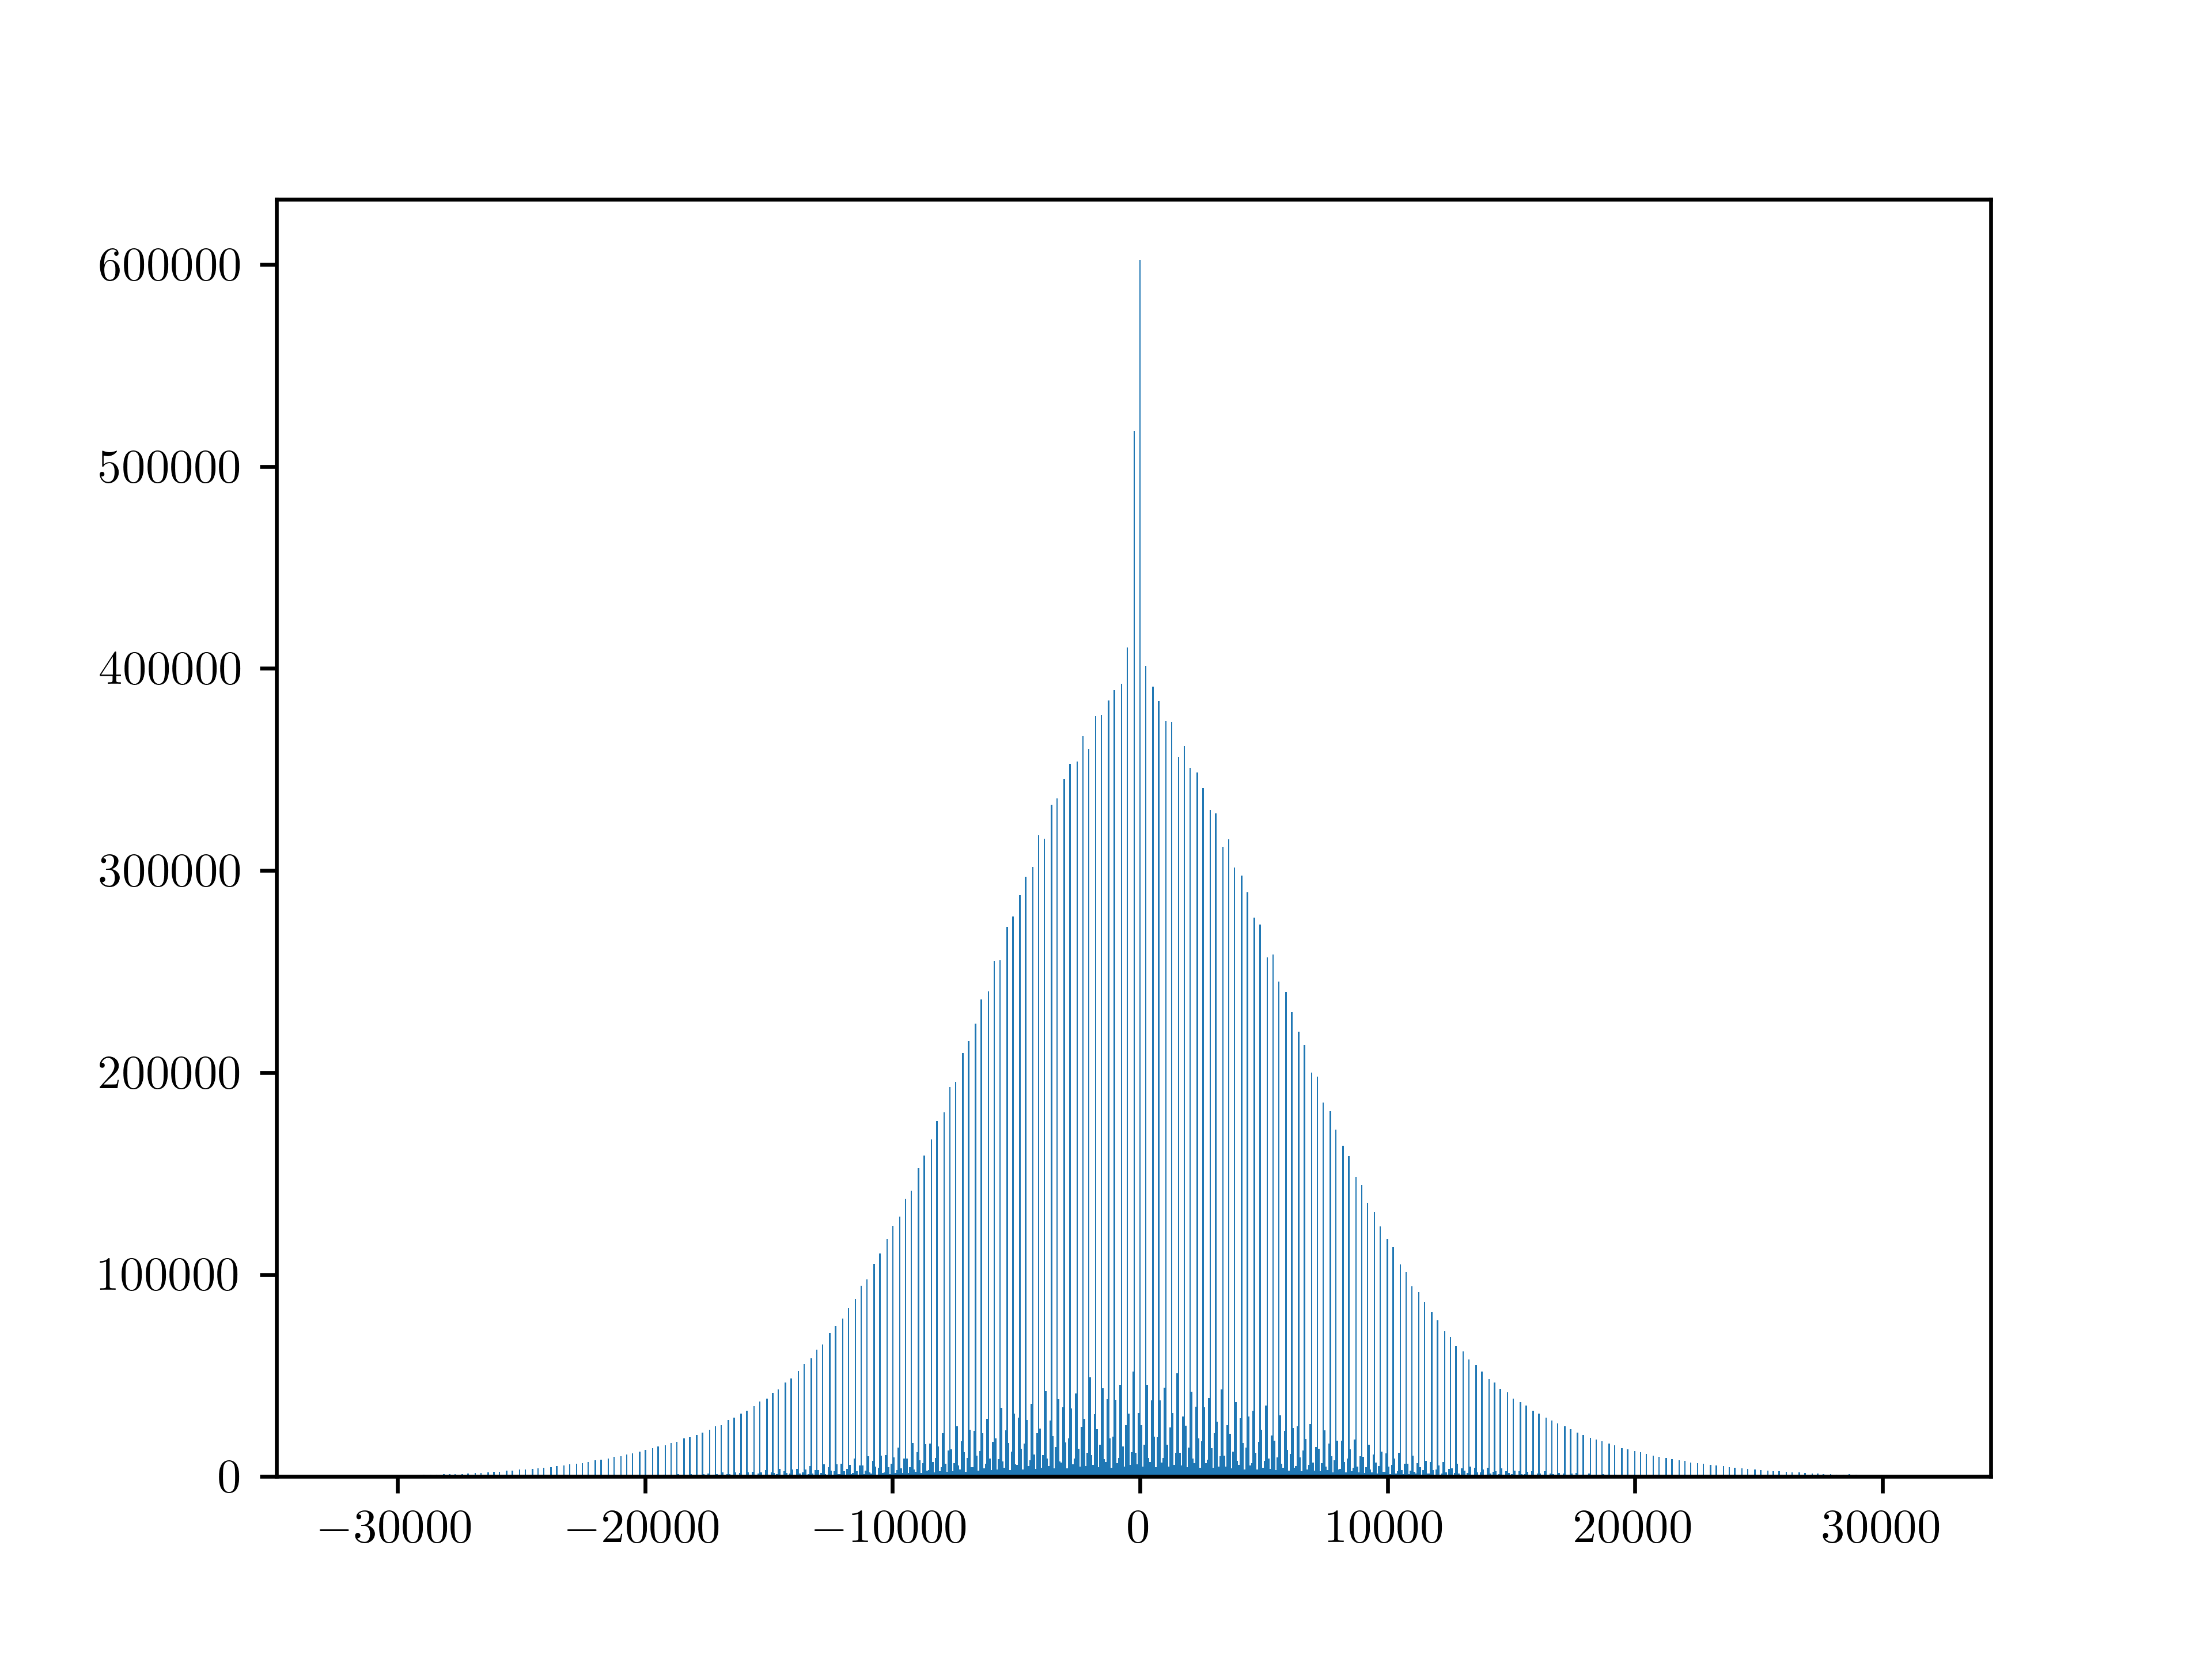
\includegraphics[width=\textwidth]{decrypted1Histogram.png}
            \caption{Decrypted}
            \label{fig:decrypted1Histogram}
        \end{center}
    \end{subfigure}
    \caption{Histogram of Audio 1: (\ref{fig:embedded1Histogram}) before encryption, (\ref{fig:encrypted1Histogram}) after encryption and (\ref{fig:decrypted1Histogram}) after decryption.}
    \label{fig:audio1Histogram}
\end{figure}
\begin{figure}[pos=h]
    \begin{subfigure}[h]{0.3\textwidth}
        \begin{center}
            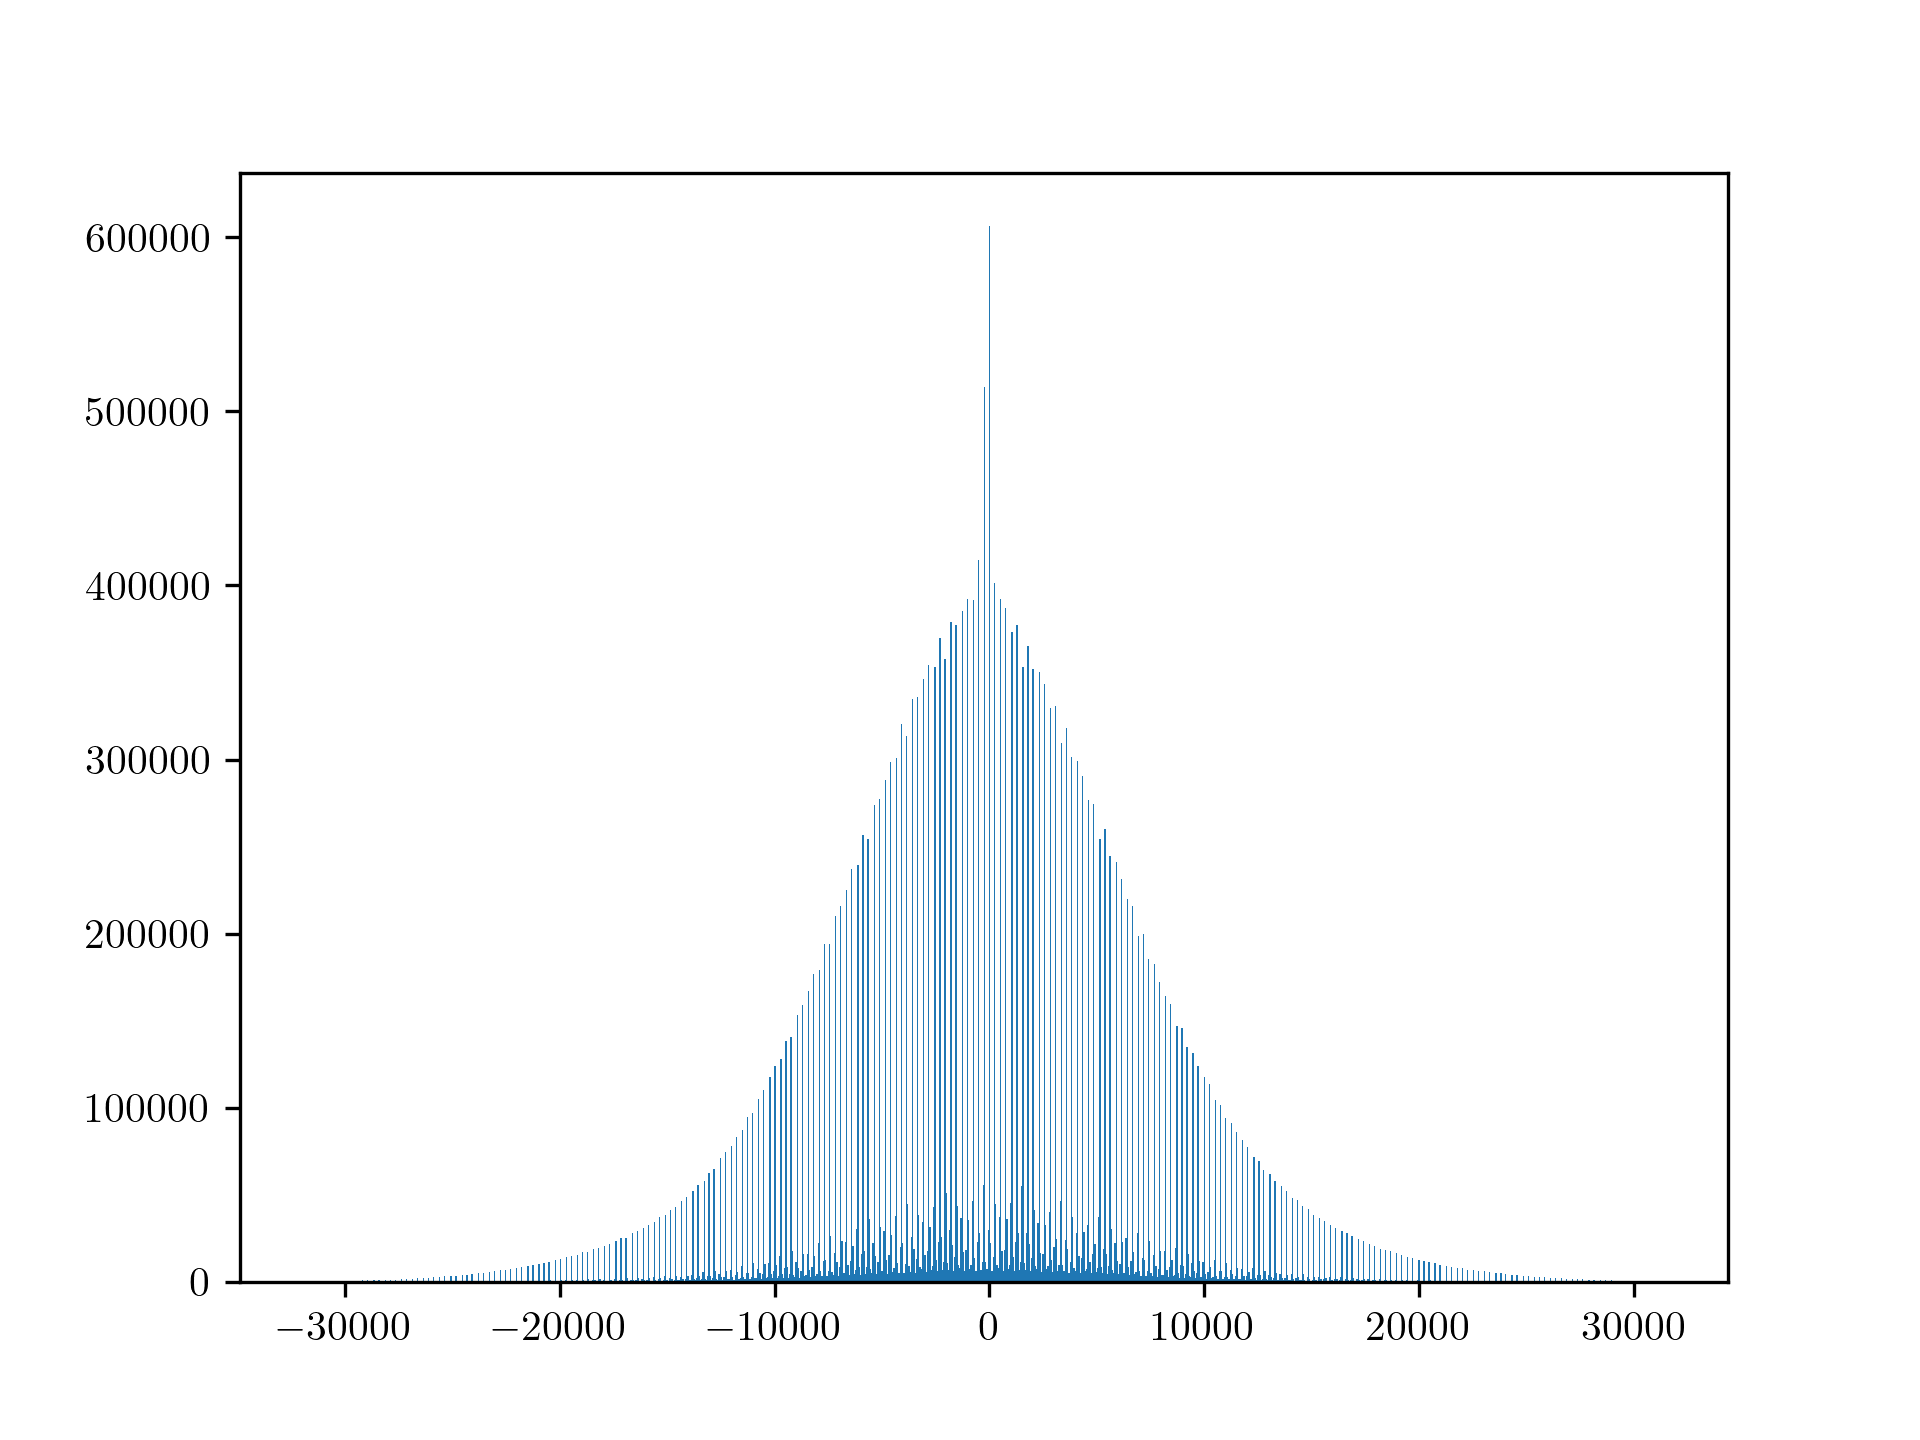
\includegraphics[width=\textwidth]{embedded2Histogram.png}
            \caption{Original}
            \label{fig:embedded2Histogram}
        \end{center}
    \end{subfigure}
    \begin{subfigure}[h]{0.3\textwidth}
        \begin{center}
            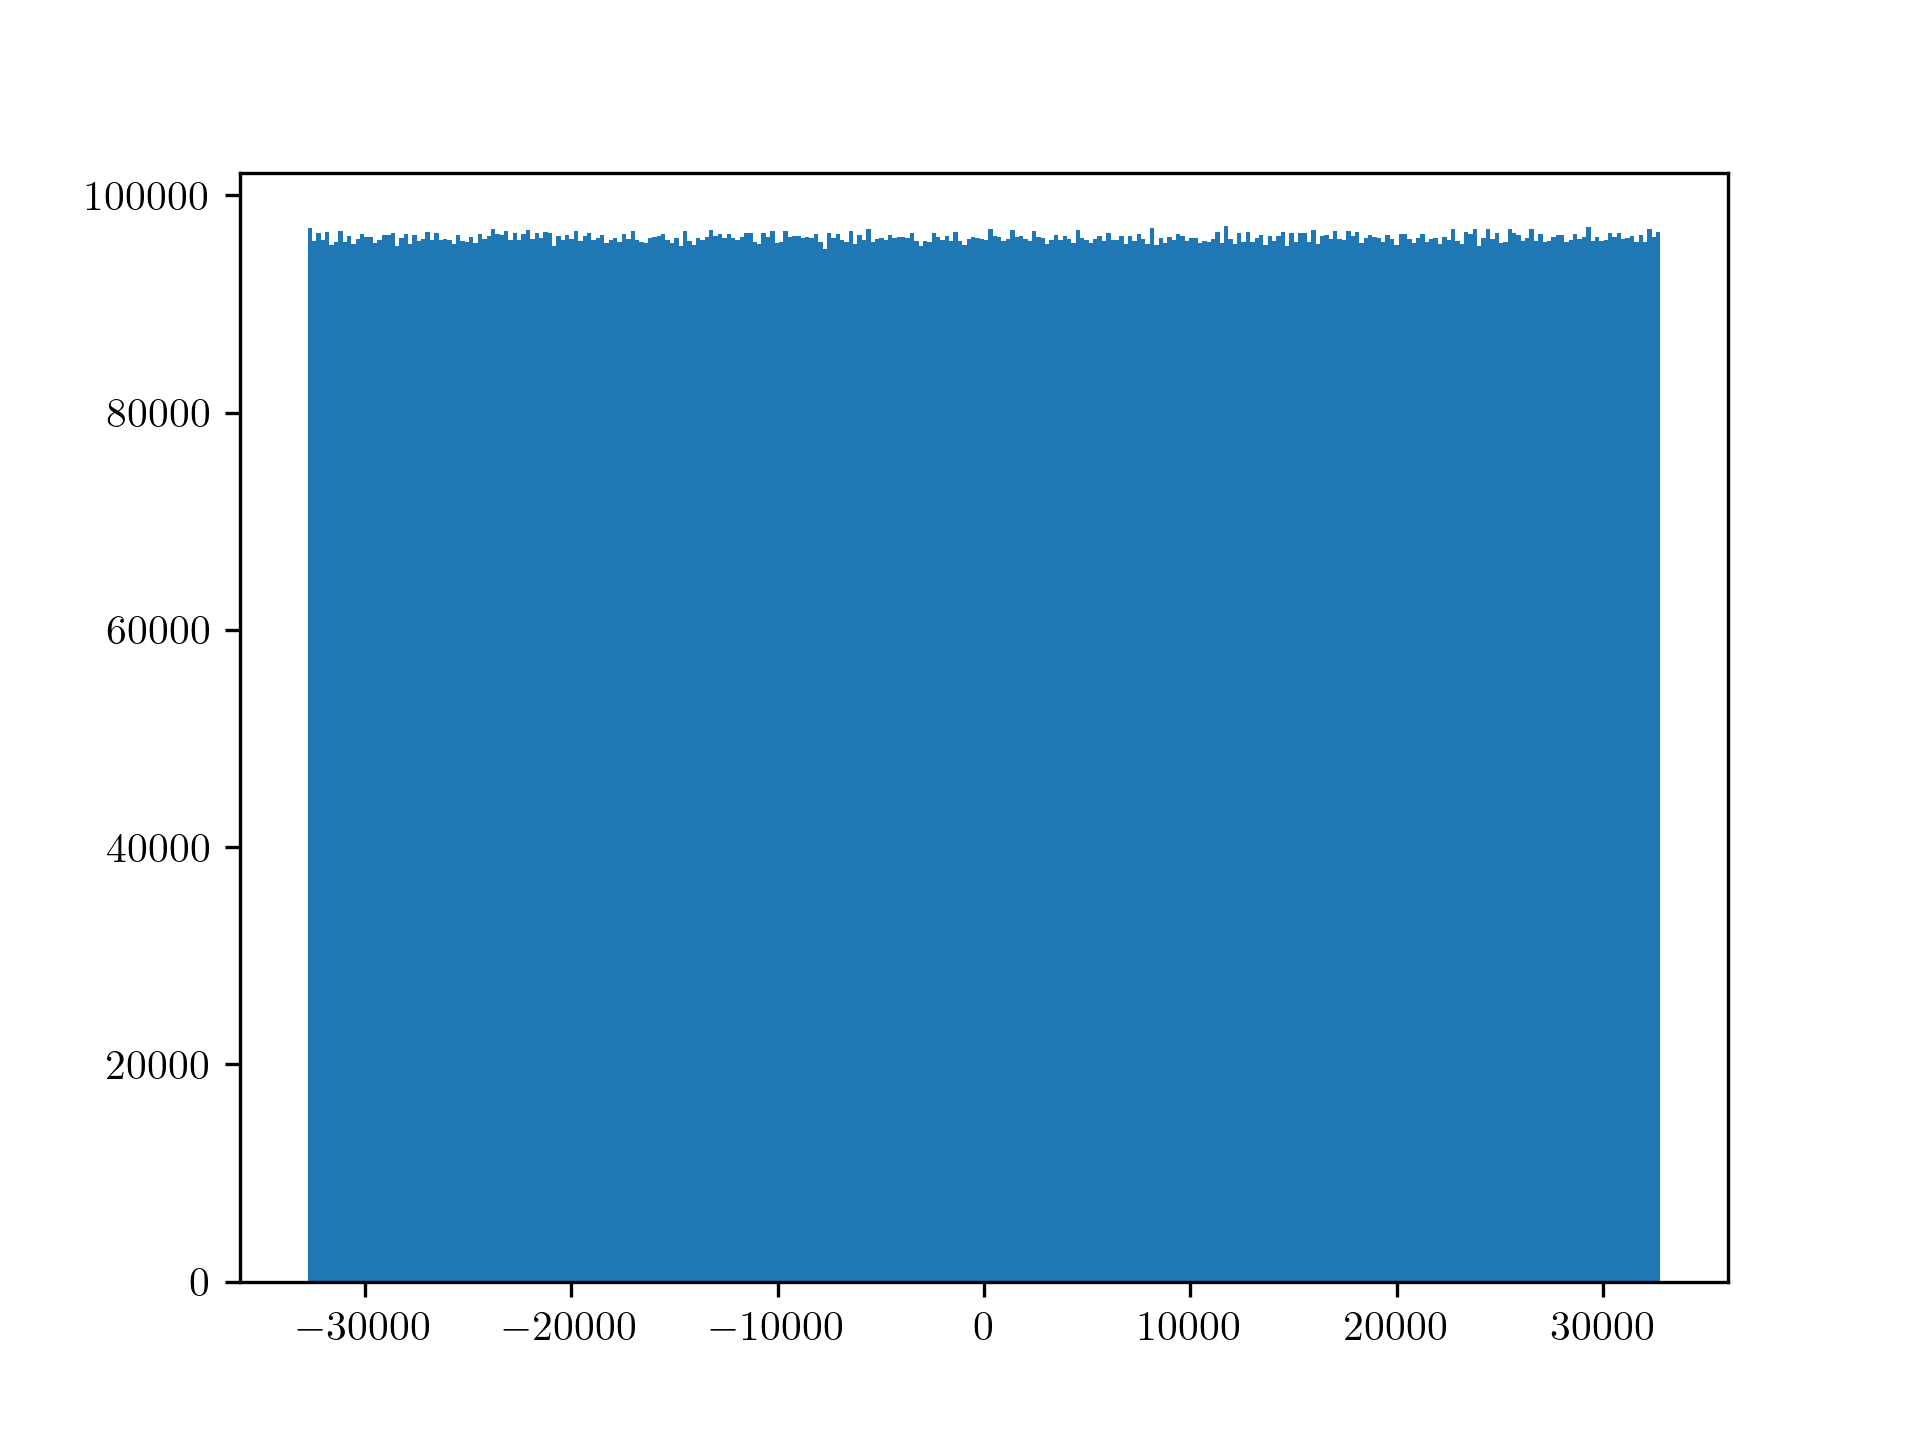
\includegraphics[width=\textwidth]{encrypted2Histogram.png}
            \caption{Encrypted}
            \label{fig:encrypted2Histogram}
        \end{center}
    \end{subfigure}
    \begin{subfigure}[h]{0.3\textwidth}
        \begin{center}
            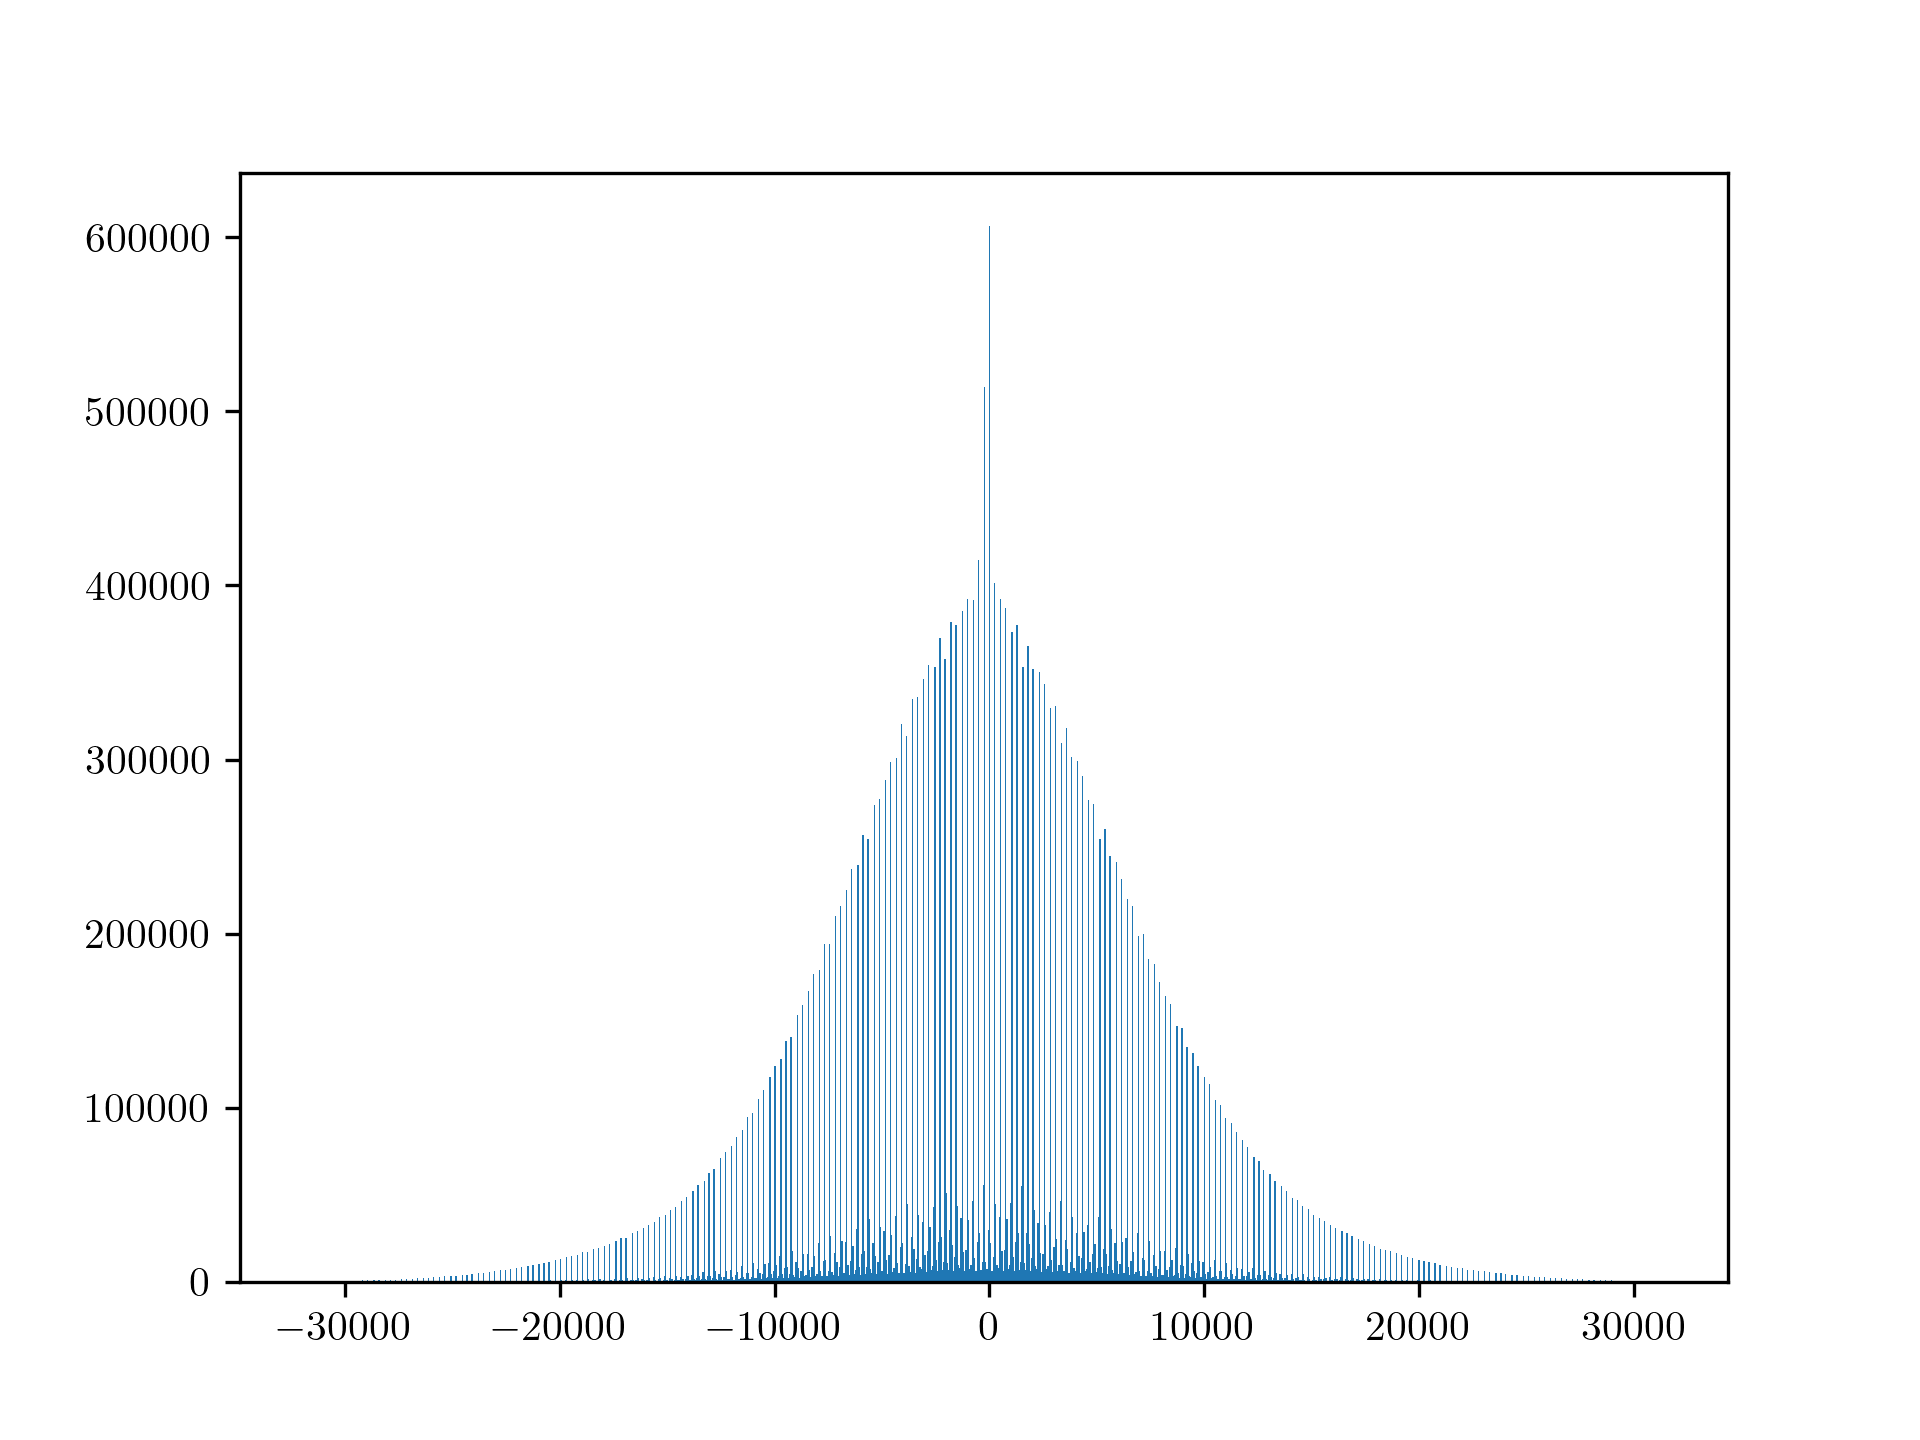
\includegraphics[width=\textwidth]{decrypted2Histogram.png}
            \caption{Decrypted}
            \label{fig:decrypted2Histogram}
        \end{center}
    \end{subfigure}
    \caption{Histogram of Audio 2: (\ref{fig:embedded2Histogram}) before encryption, (\ref{fig:encrypted2Histogram}) after encryption and (\ref{fig:decrypted2Histogram}) after decryption.}
    \label{fig:audio2Histogram}
\end{figure}
The histograms depicted in Figures \ref{fig:audio1Histogram} and \ref{fig:audio2Histogram} demonstrate a significant difference between the embedded and encrypted audio signals, confirming the effectiveness of the encryption process. In contrast, the similarity between the histograms of the embedded and decrypted audio signals (Figures \ref{fig:embedded1Histogram} and \ref{fig:decrypted1Histogram}, and Figures \ref{fig:embedded2Histogram} and \ref{fig:decrypted2Histogram}) verifies the accuracy of the decryption process. Moreover, the visual similarity between the histograms of the embedded and decrypted audio signals provides strong evidence for the reliability of the steganography scheme.
\subsubsection{Spectrogram Analysis}
Spectrogram is a visual representation of the variation of the spectrum of frequencies of a signal with respect to time. Figure \ref{fig:audio1Spectrogram} and \ref{fig:audio2Spectrogram} shows the histogram before encryption, after encryption and after encryption of Audio 1 and Audio 2 produced through steganography, respectively.
\begin{figure}[pos=h]
    \begin{subfigure}[h]{0.3\textwidth}
        \begin{center}
            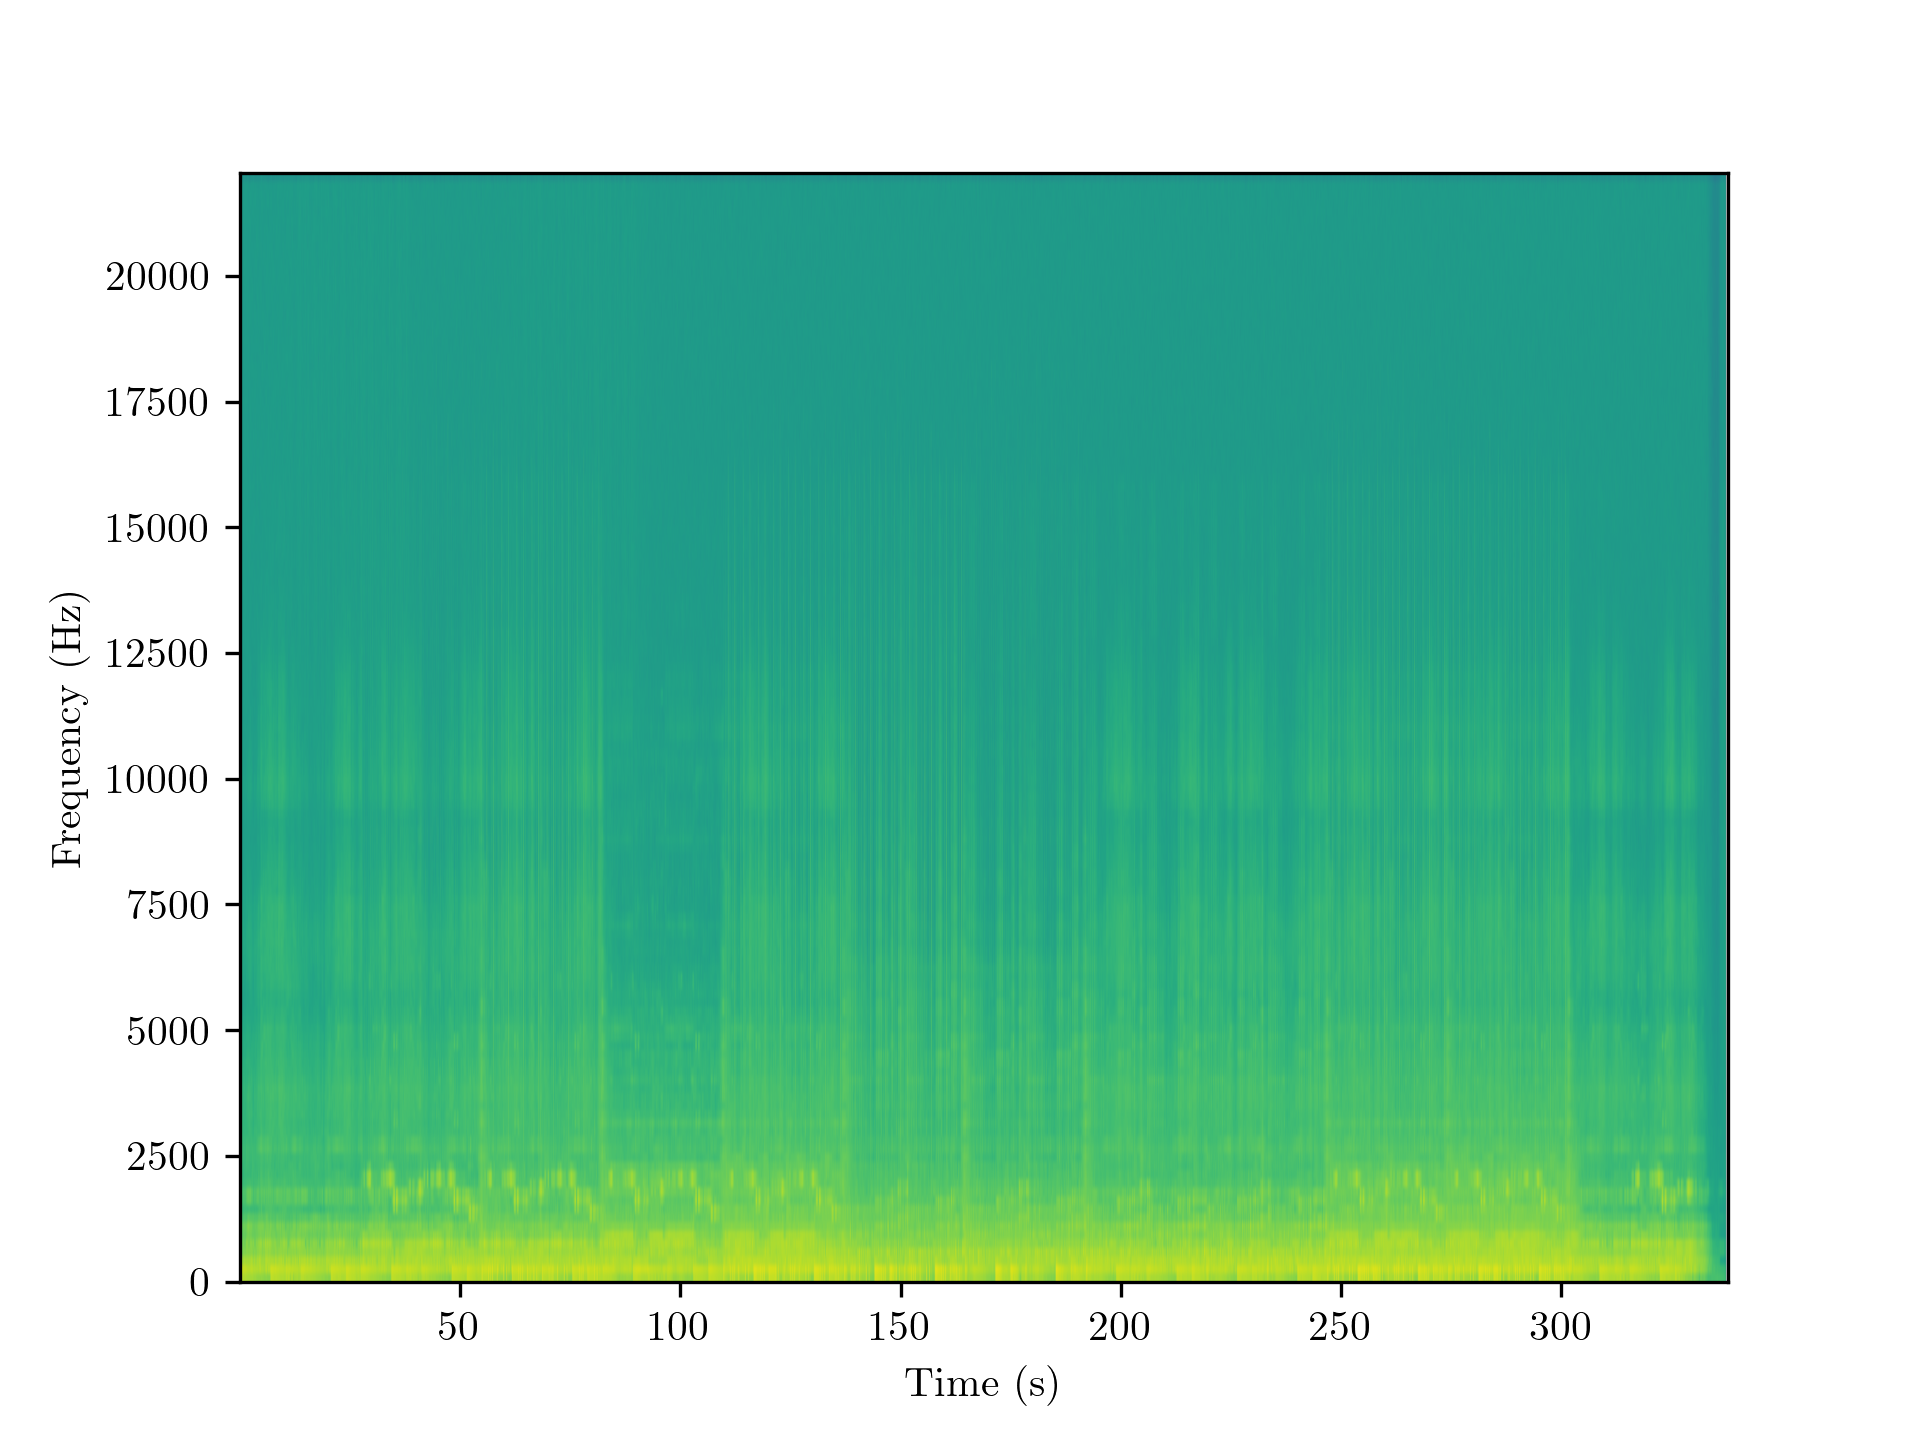
\includegraphics[width=\textwidth]{embedded1Spectrogram.png}
            \caption{Original}
            \label{fig:embedded1Spectrogram}
        \end{center}
    \end{subfigure}
    \begin{subfigure}[h]{0.3\textwidth}
        \begin{center}
            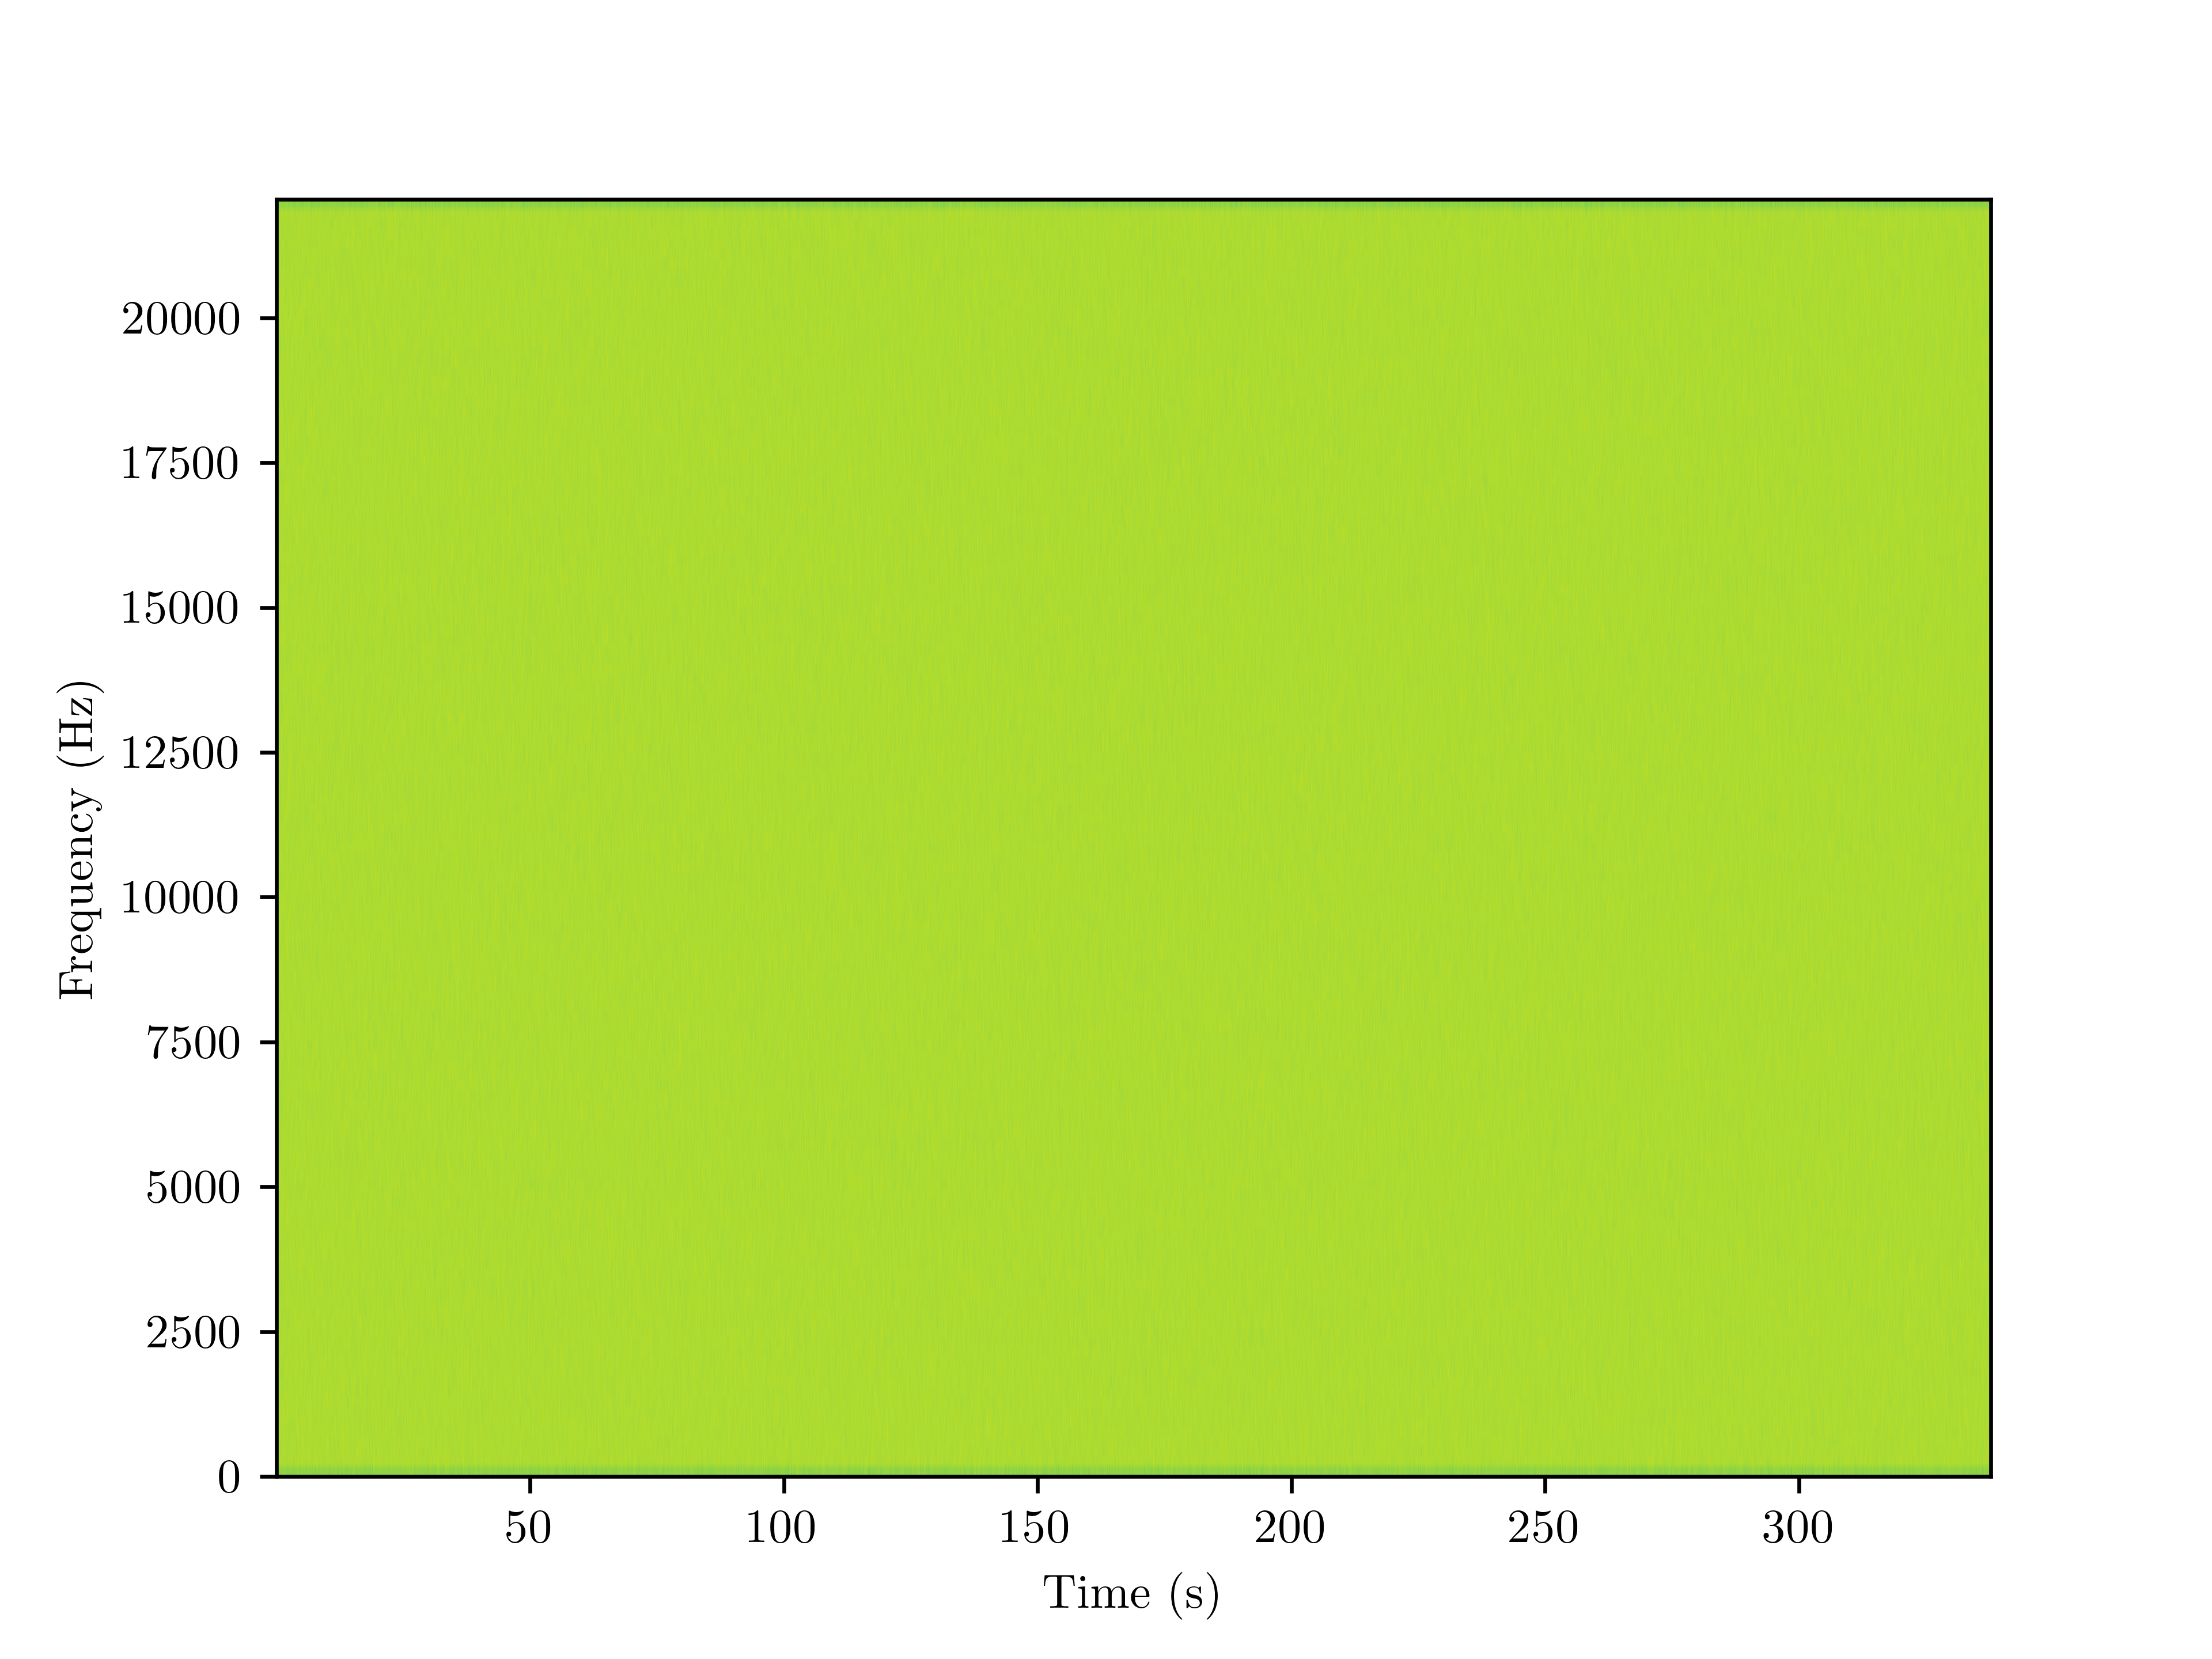
\includegraphics[width=\textwidth]{encrypted1Spectrogram.png}
            \caption{Encrypted}
            \label{fig:encrypted1Spectrogram}
        \end{center}
    \end{subfigure}
    \begin{subfigure}[h]{0.3\textwidth}
        \begin{center}
            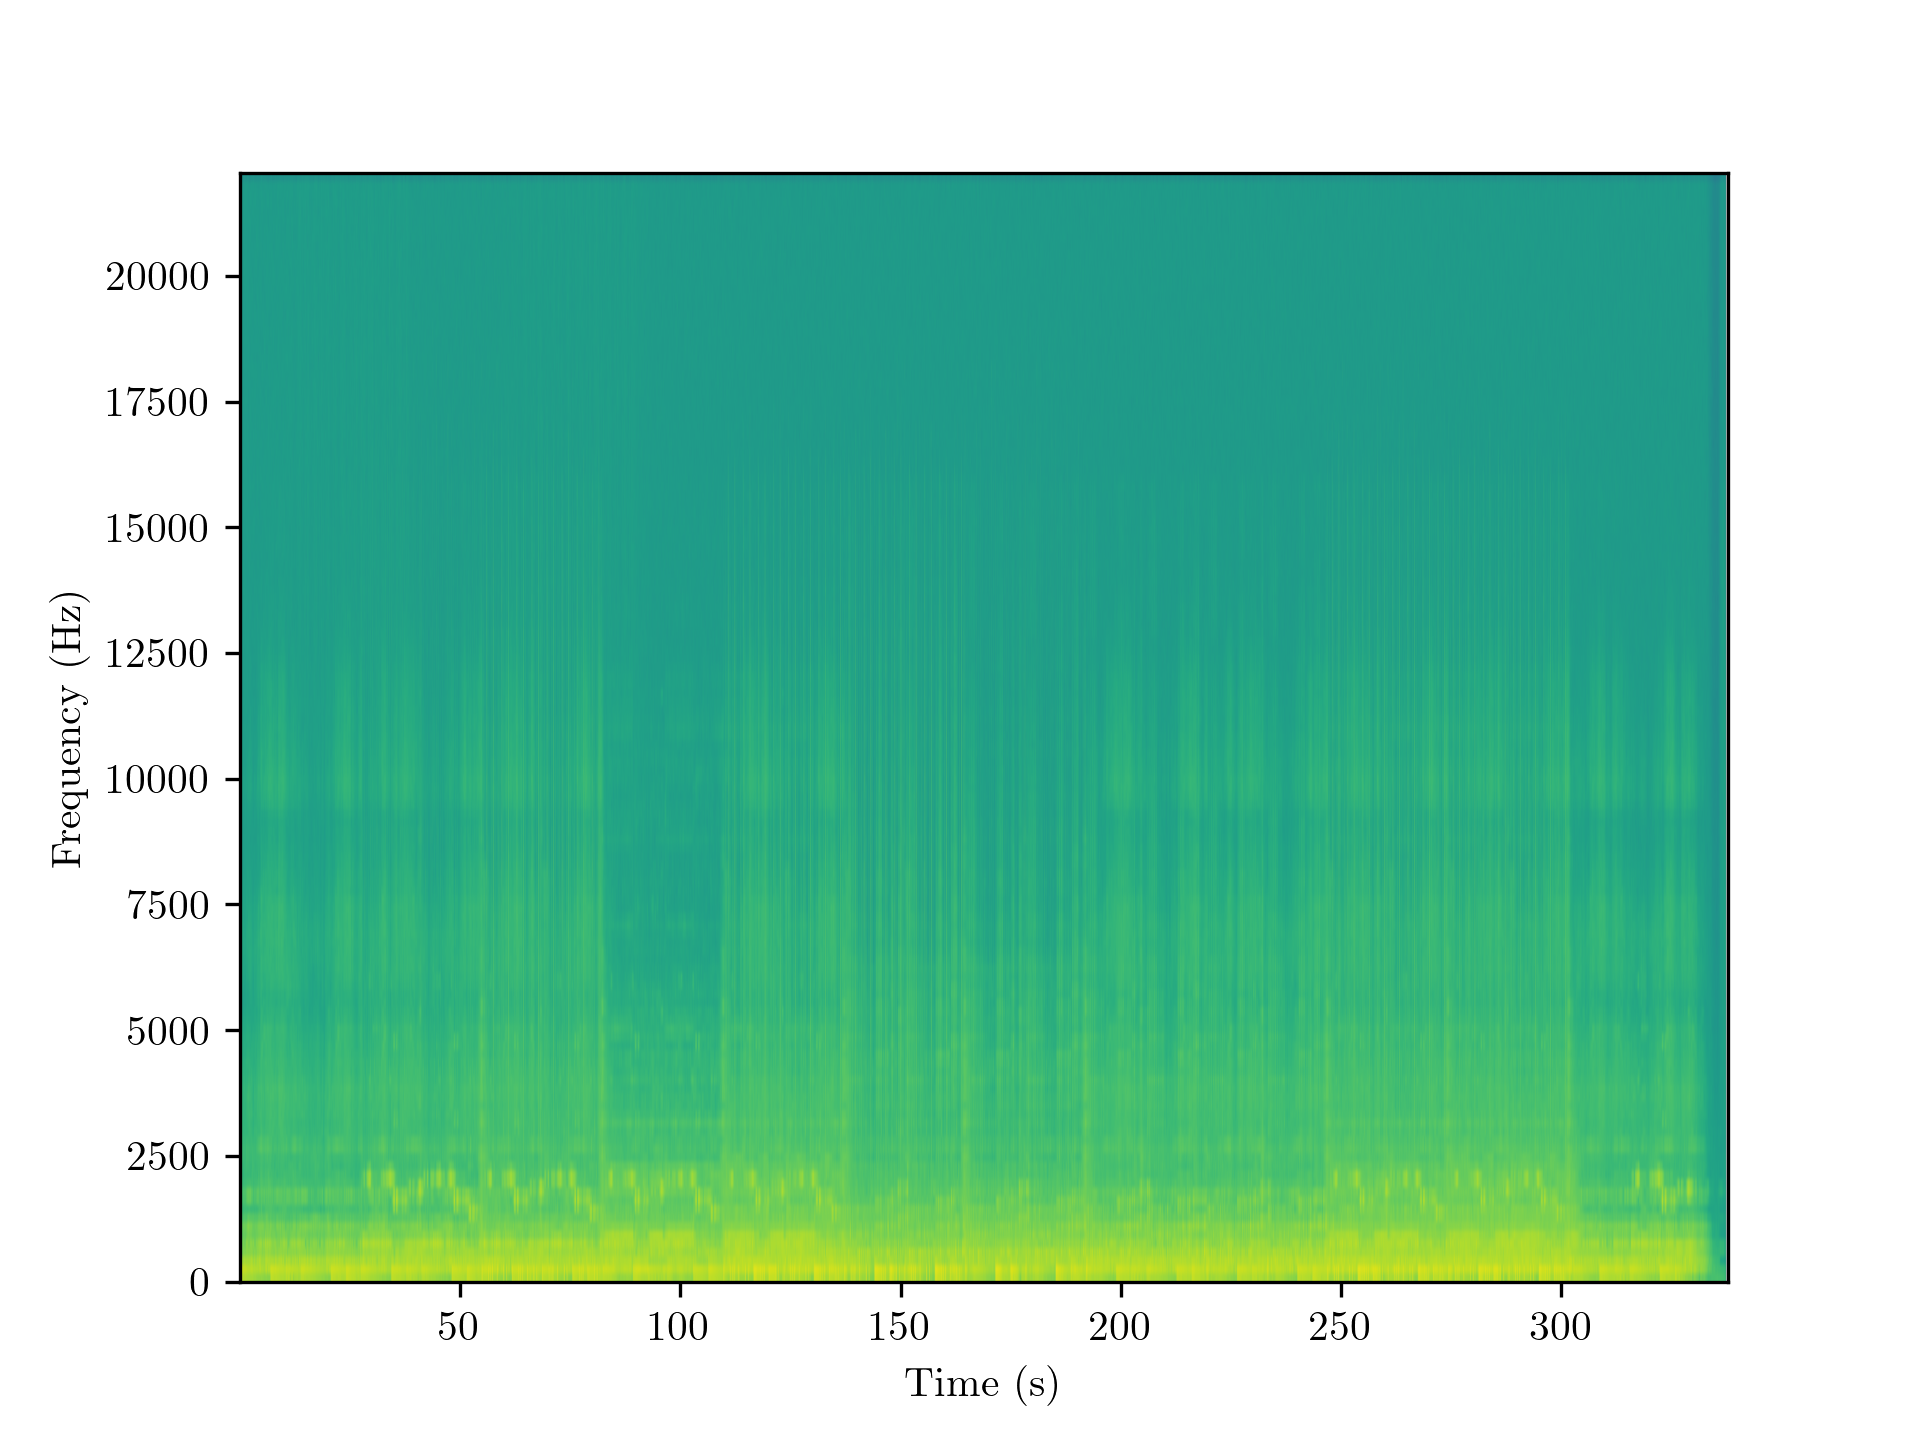
\includegraphics[width=\textwidth]{decrypted1Spectrogram.png}
            \caption{Decrypted}
            \label{fig:decrypted1Spectrogram}
        \end{center}
    \end{subfigure}
    \caption{Spectrogram of Audio 1: (\ref{fig:embedded1Spectrogram}) before encryption, (\ref{fig:encrypted1Spectrogram}) after encryption and (\ref{fig:decrypted1Spectrogram}) after decryption.}
    \label{fig:audio1Spectrogram}
\end{figure}
\begin{figure}[pos=h]
    \begin{subfigure}[h]{0.3\textwidth}
        \begin{center}
            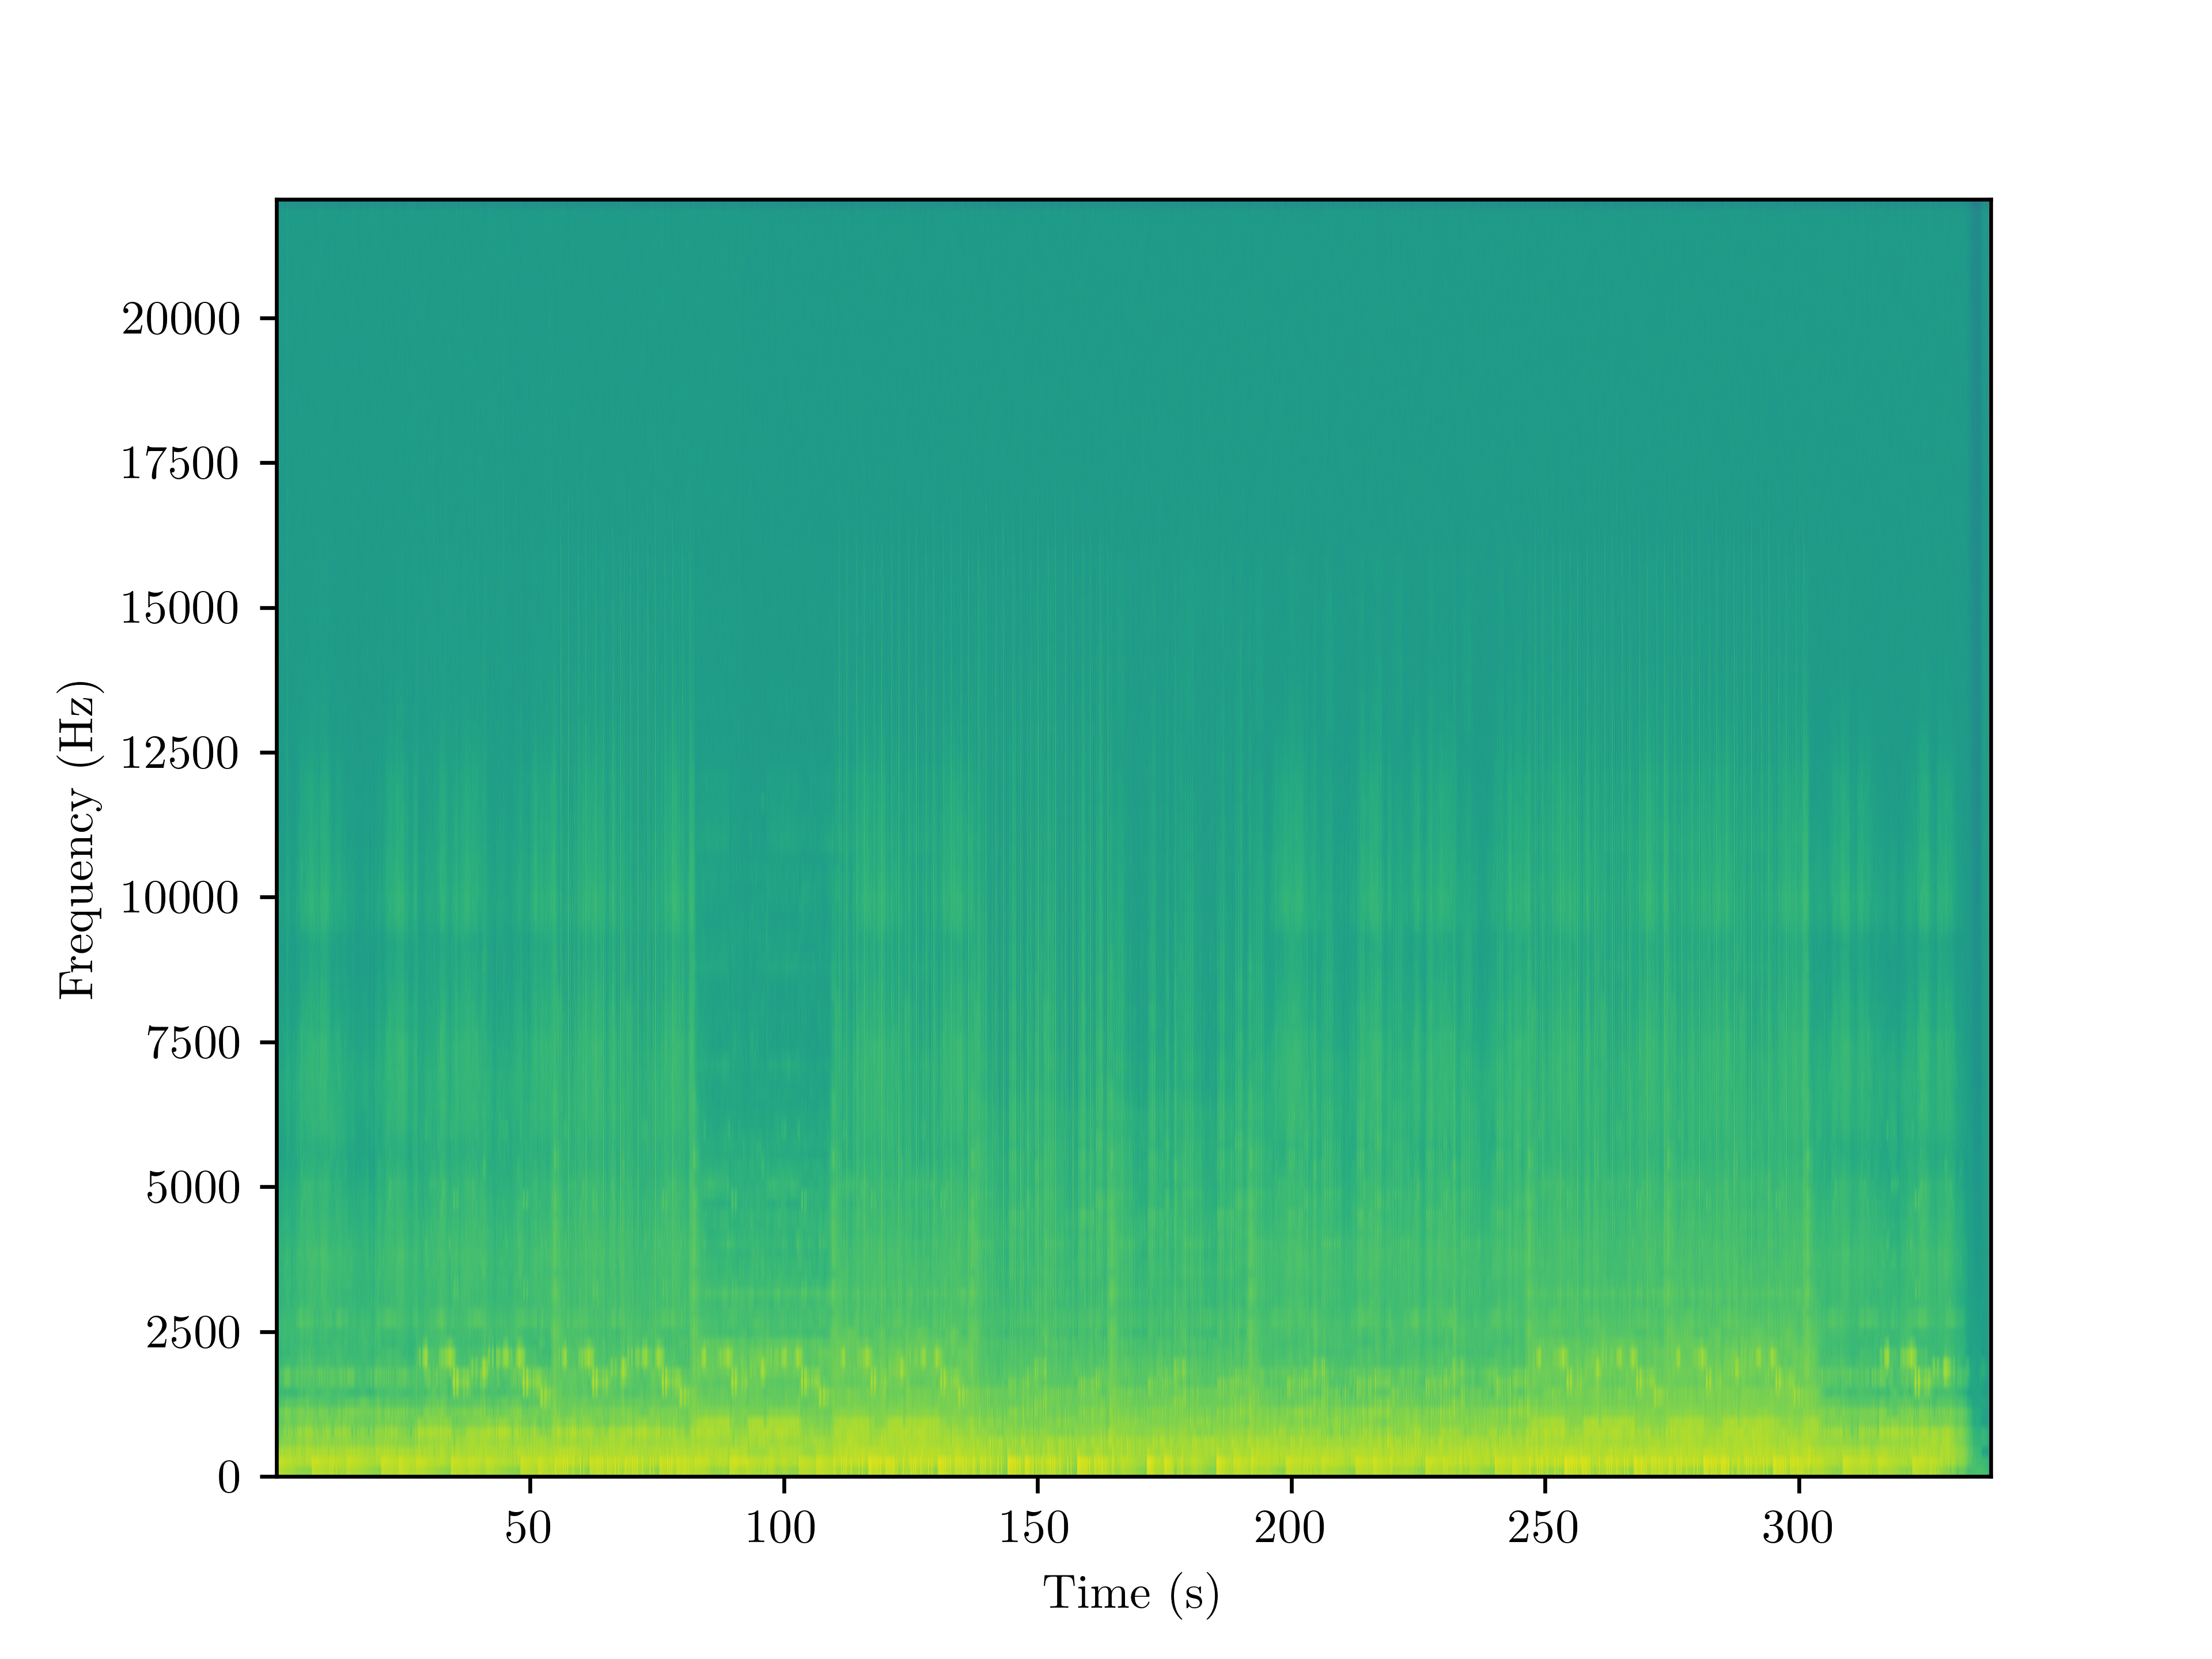
\includegraphics[width=\textwidth]{embedded2Spectrogram.png}
            \caption{Original}
            \label{fig:embedded2Spectrogram}
        \end{center}
    \end{subfigure}
    \begin{subfigure}[h]{0.3\textwidth}
        \begin{center}
            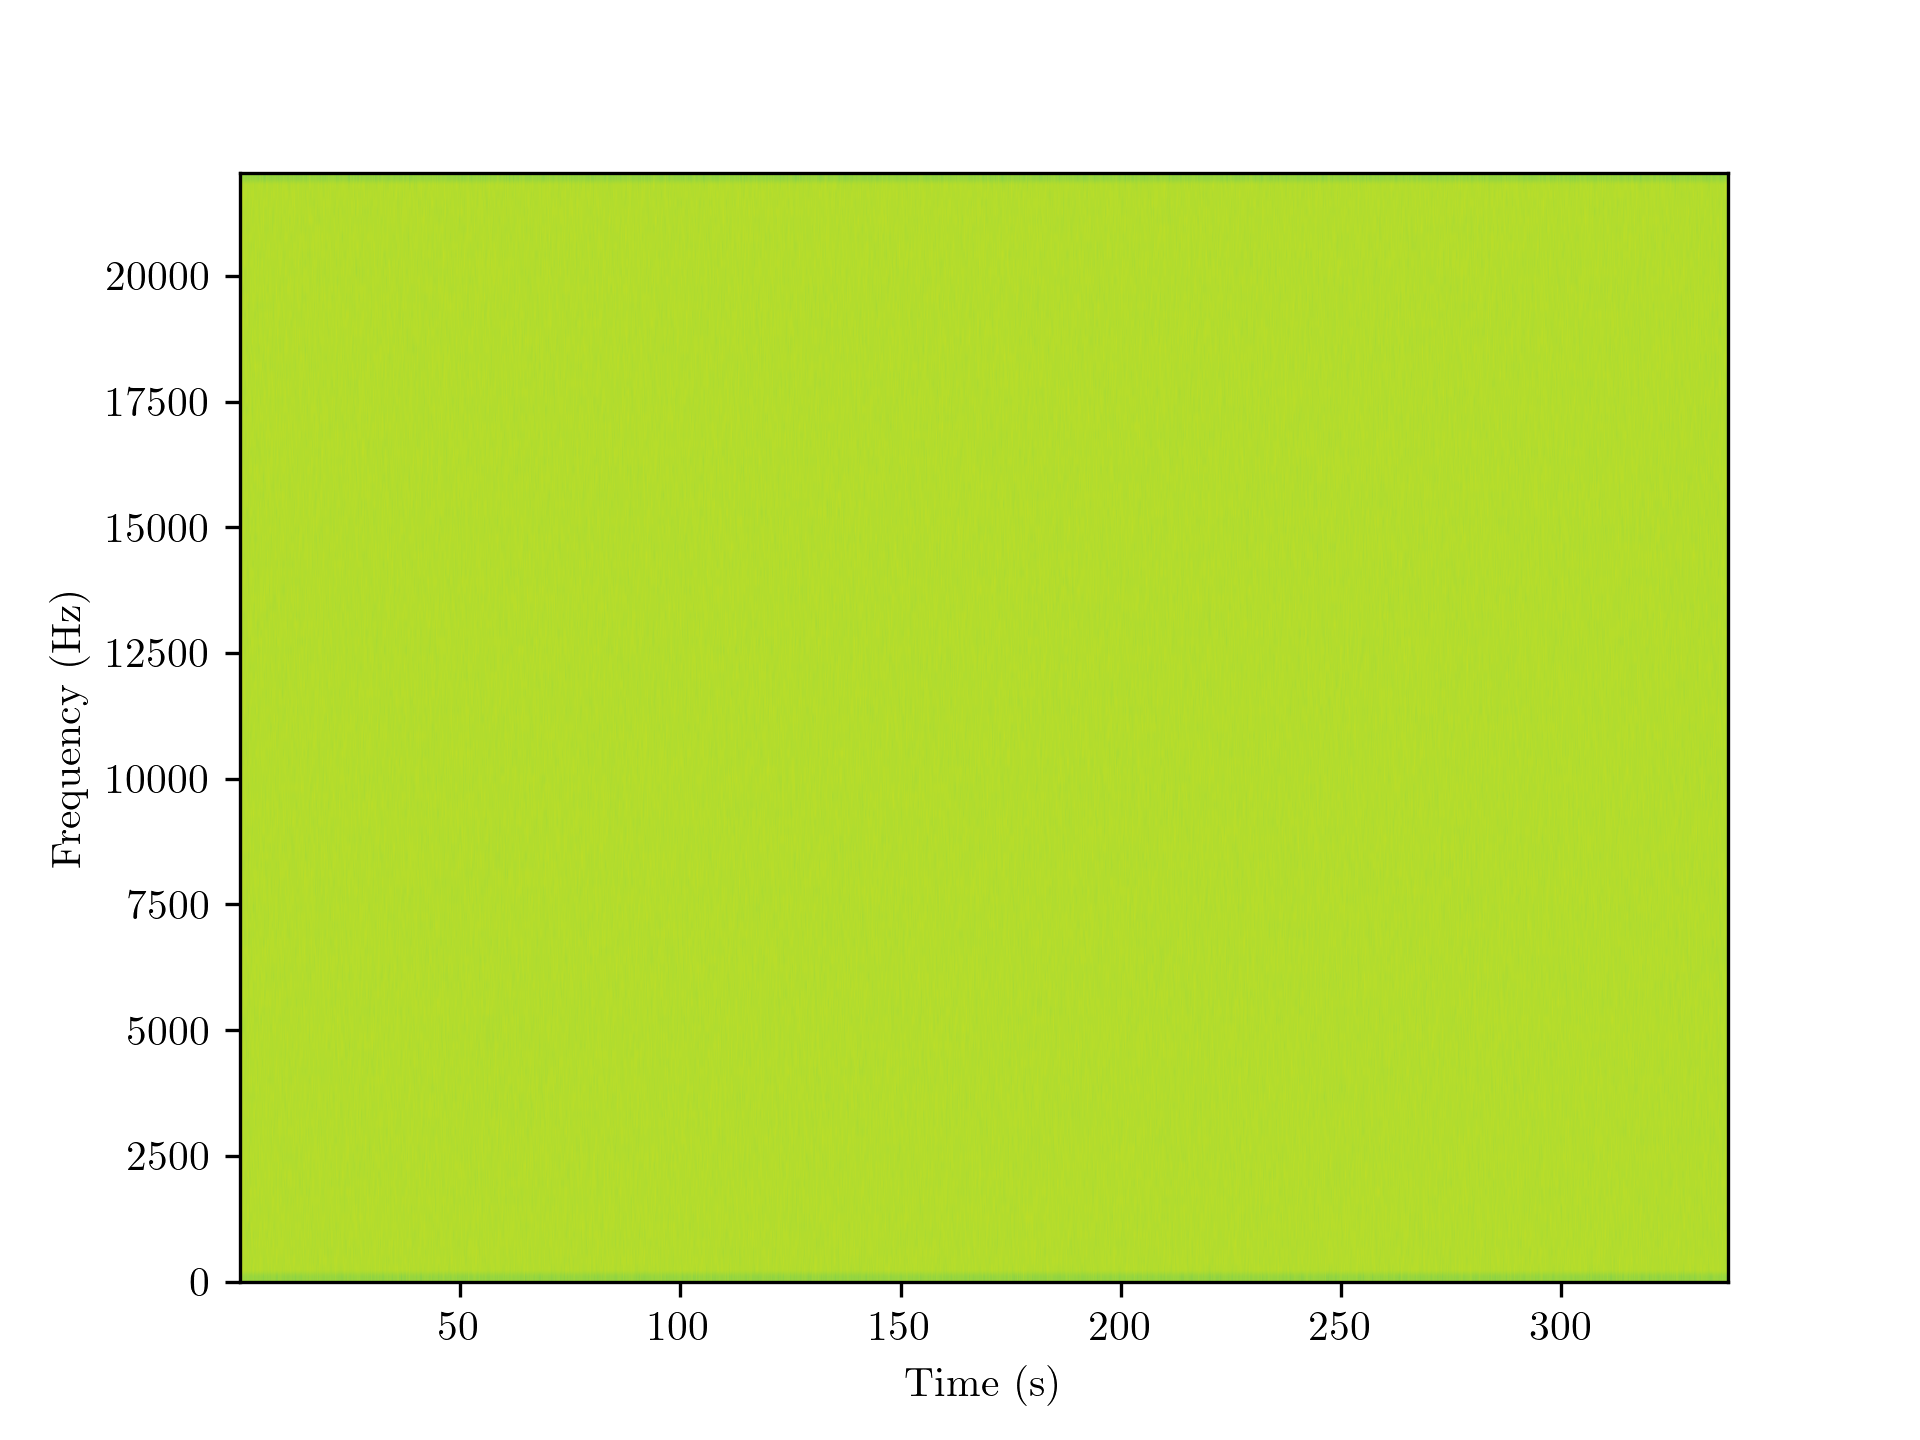
\includegraphics[width=\textwidth]{encrypted2Spectrogram.png}
            \caption{Encrypted}
            \label{fig:encrypted2Spectrogram}
        \end{center}
    \end{subfigure}
    \begin{subfigure}[h]{0.3\textwidth}
        \begin{center}
            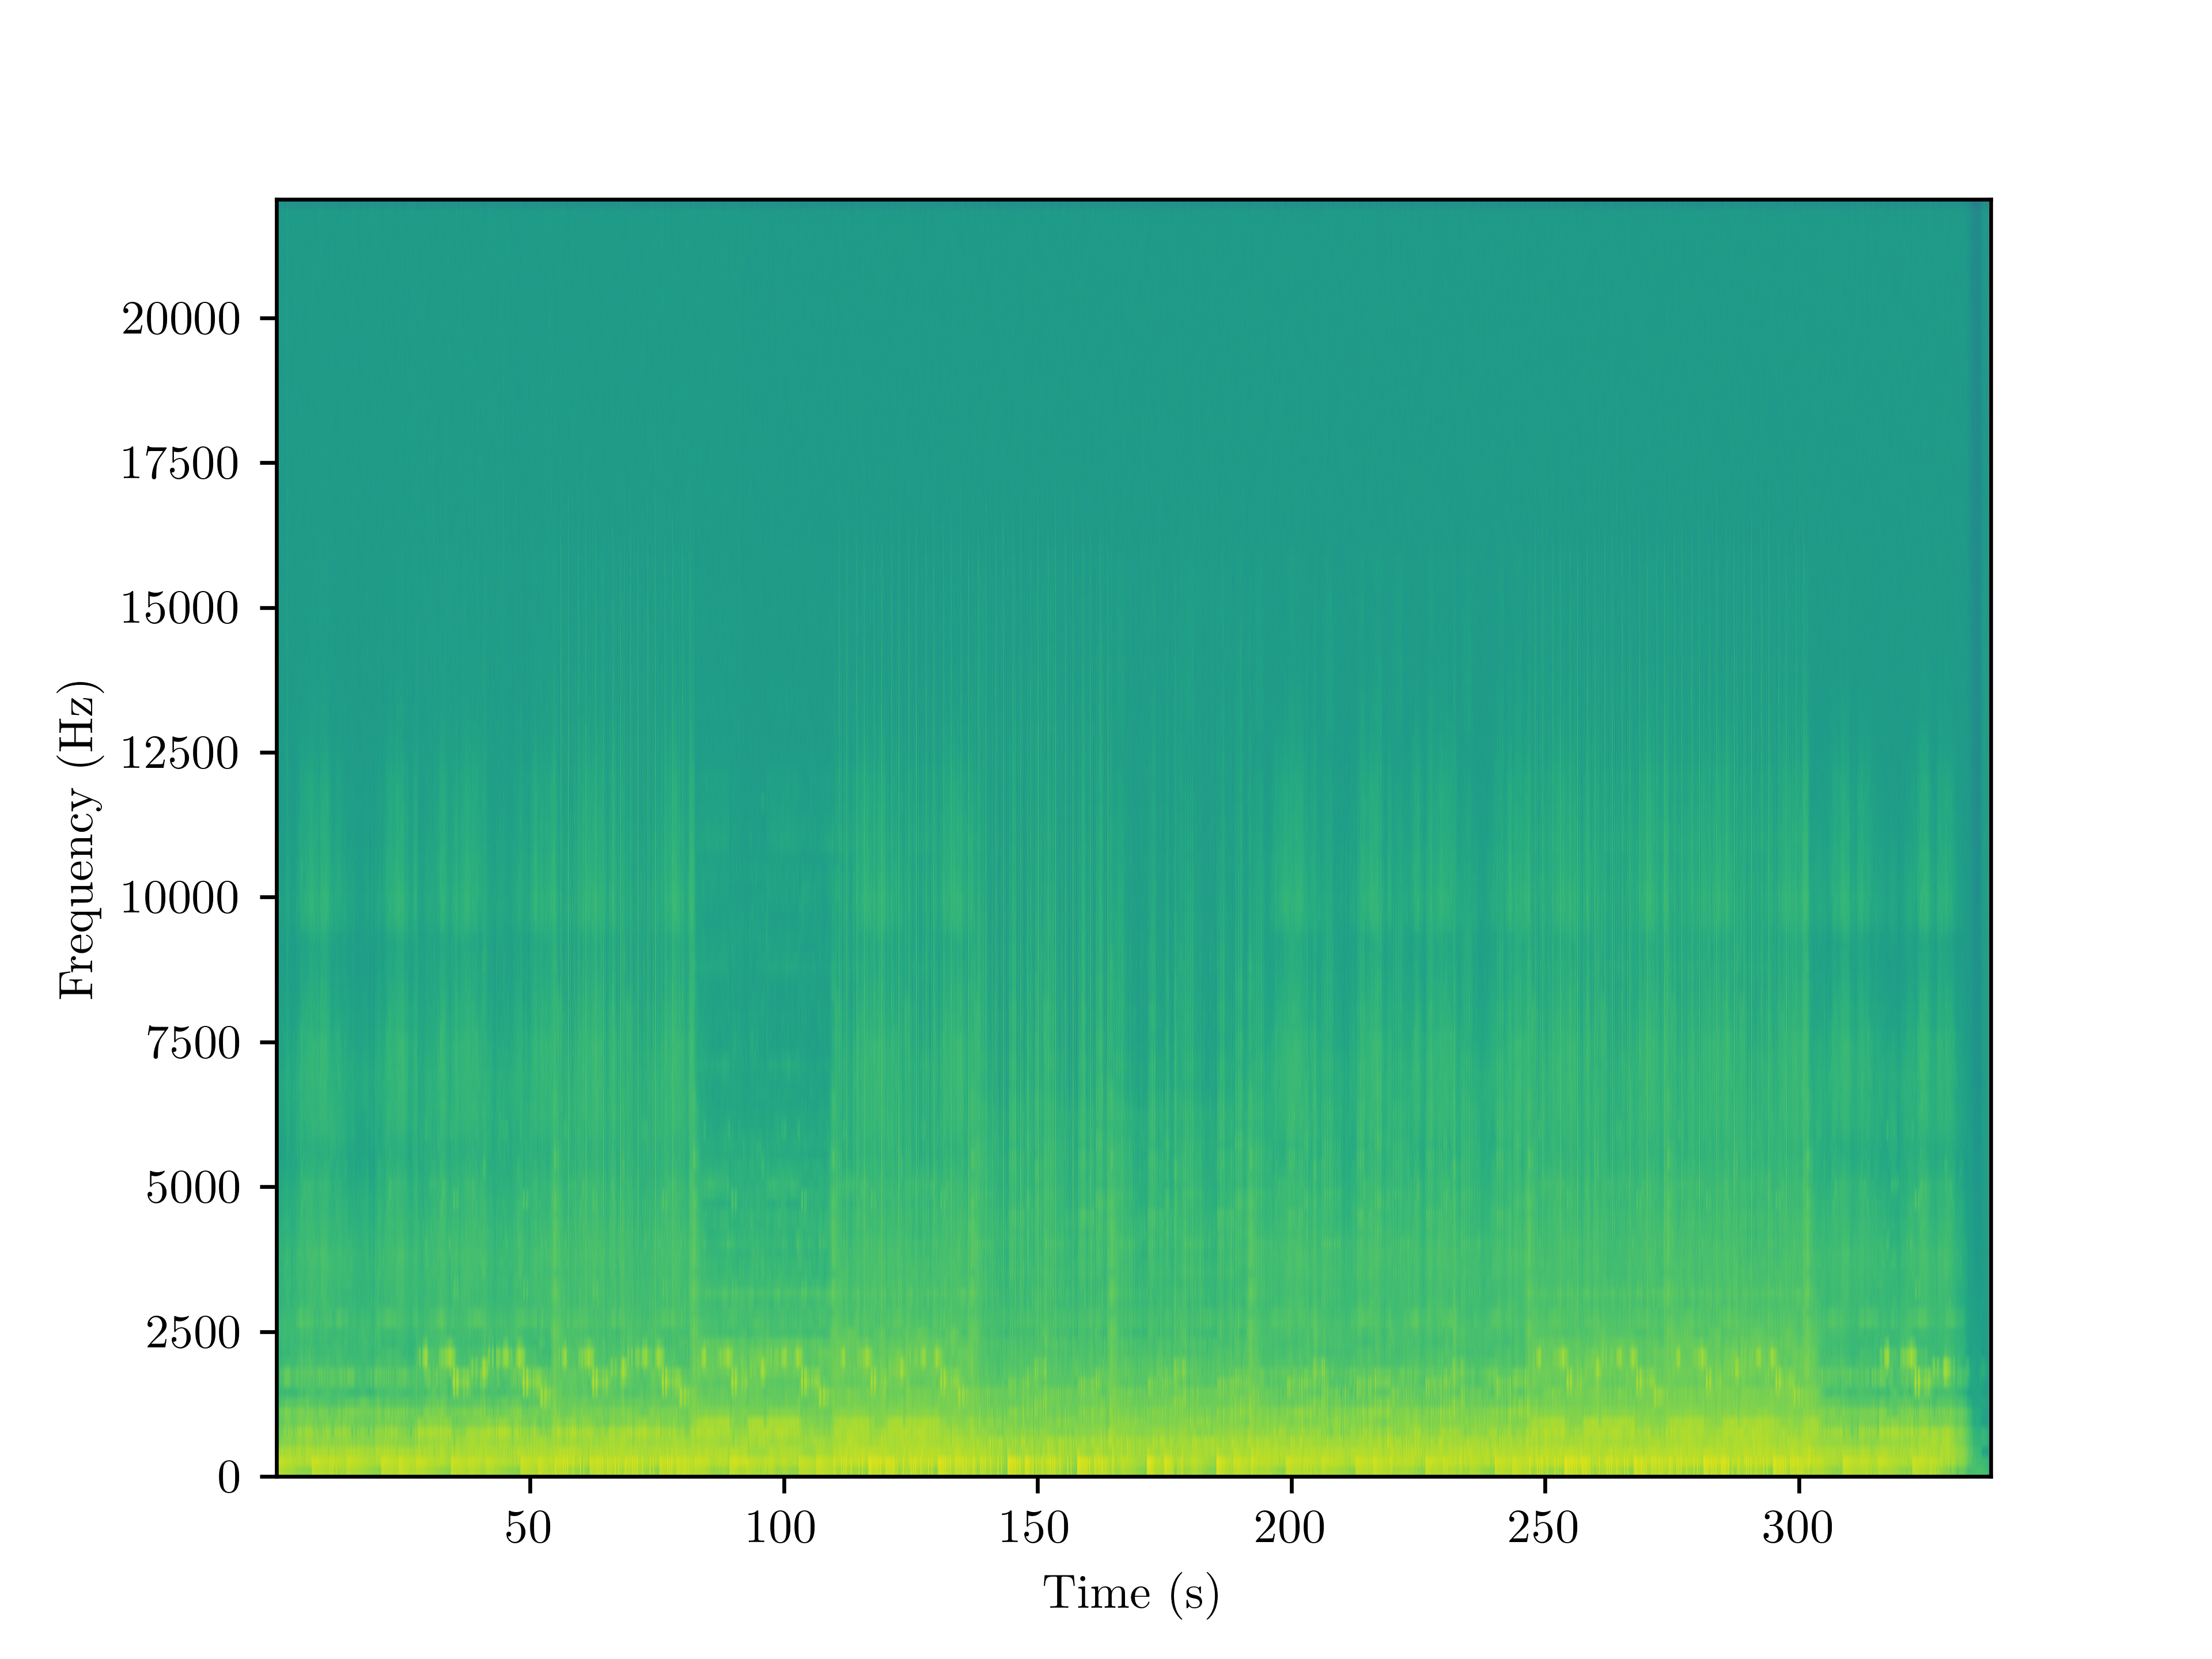
\includegraphics[width=\textwidth]{decrypted2Spectrogram.png}
            \caption{Decrypted}
            \label{fig:decrypted2Spectrogram}
        \end{center}
    \end{subfigure}
    \caption{Spectrogram of Audio 2: (\ref{fig:embedded2Spectrogram}) before encryption, (\ref{fig:encrypted2Spectrogram}) after encryption and (\ref{fig:decrypted2Spectrogram}) after decryption.}
    \label{fig:audio2Spectrogram}
\end{figure}

A visual inspection of the spectrograms in Figures \ref{fig:audio1Spectrogram} and \ref{fig:audio2Spectrogram} reveals a stark contrast between the embedded and encrypted audio signals, indicating successful encryption. Conversely, the spectrograms of the embedded and decrypted audio signals (Figures \ref{fig:embedded1Spectrogram} and \ref{fig:decrypted1Spectrogram}, and Figures \ref{fig:embedded2Spectrogram} and \ref{fig:decrypted2Spectrogram}) exhibit a high degree of similarity, confirming the correctness of the decryption process. The striking resemblance between these correlation maps also underscores the efficacy of the steganography scheme, demonstrating its ability to conceal and retrieve the embedded audio signals accurately.
\subsubsection{Key Sensitivity Analysis}
Key Sensitivity is a measure of the response to the slightest change in key of an encryption system. High Key Sensitivity is an indication of the slightest change in encryption key causing huge changes in the encryption and decryption process. To demonstrate Key Sensitivity of the proposed architecture, let us consider two scenarios --
\begin{itemize}
    \item \textbf{Scenario -- 1:} The stego-audio is encrypted using K1 key and decrypted using the same key (Figure \ref{fig:keySensitivityK1}).
    \item \textbf{Scenario -- 2:} The stego-audio is encrypted using K1 key but decryption is attempted using K2 key, which differs from K1 by a single bit.(Figure \ref{fig:keySensitivityK2})
\end{itemize}
For instance, let $K1=\mathbf{0}0001000000100001010001011000011$ and $K2=\mathbf{1}0001000000100001010001011000011$. The hash output are $\text{SHA3}_{K1}=e57179067dc01f3d3434e4e1447d0368cd716894c71ca9e59da3d7b9a5be6fce$ and $\text{SHA3}_{K2}=a2b702be844ae3adea1fd88c1c6e2452fdde129988fd78f047ebacf5c5d2aa67$. Due to the mismatch in computed hexdigest, decryption attempt with $K2$ will fail.
\begin{figure}[pos=h]
    \begin{center}
        \includesvg[width=\textwidth]{keySensitivityK1.svg}
        \caption{Key Sensitivity Analysis Scenario 1: Encryption and Decryption using the same key, $K1$}
        \label{fig:keySensitivityK1}
    \end{center}
\end{figure}
\begin{figure}[pos=h]
    \begin{center}
        \includesvg[width=0.75\textwidth]{keySensitivityK2.svg}
        \caption{Key Sensitivity Analysis Scenario 2: Encryption using key $K1$ and Decryption using key $K2$}
        \label{fig:keySensitivityK2}
    \end{center}
\end{figure}
\subsubsection{Unified Average Changing Intensity (UACI)}
Unified Average Changing Intensity is a measure of the average intensity change rate between the original and the modified signal. In this case, UACI measures the average intensity change rate between the embedded audio and the encrypted audio signals. A higher UACI value is preferred, as a higher UACI value indicates a considerable change in the encrypted audio from the original embedded audio. For $16$-bit audio signals, UACI is calculated using the following formula --
\begin{equation}
    \text{UACI}=\frac{1}{N}\sum_{i=1}^{N}\left(\frac{|S_i-D_i|}{65535}\right)\times100
\end{equation}
Here, $S_i$ is the samples of the embedded signal, $D_i$ is the samples of the encrypted signals and $N$ is the total number of samples, which is the same in both signals. The calculated values of UACI is shown in Table \ref{table:uaci}.
\begin{table}[pos=h]
    \begin{center}
        \caption{UACI values of audio signals.}
        \begin{tabular}{cr}
            \hline
            Audio File & \multicolumn{1}{c}{UACI}                    \\ \hline
            Audio 1    & $50.003490097286196$                        \\ \hdashline
            Audio 2    & $49.991852542937640$                        \\ \hline
                       & \textit{avg.:}$\mathbf{49.997671320111918}$
        \end{tabular}
        \label{table:uaci}
    \end{center}
\end{table}

It can be gleaned with ease from the table above that the encrypted audios almost do not contain any patterns from the original embedded audios as the UACI values were comparatively high.
\subsubsection{Number of samples change rate (NSCR)}
Number of samples change rate (NSCR) calculates the percentage of the sample values that are in contrast between the original embedded audios and the encrypted audios. Higher NSCR values are an indication of higher number of samples being altered in the course of encryption and thus producing a signal substantially different from the original signal. The following formula is utilized to determine the value of NSCR --
\begin{equation}
    \text{NSCR}=\left(\frac{D}{N}\right)\times100
\end{equation}
Here, $D$ is the number of sample that are distinct between the original embedded signal and the encrypted audio signal and $N$ is the total number of samples, which is the same in both signals. The NSCR values that we determined is shown in Table \ref{table:nscr}.
\begin{table}[pos=h]
    \begin{center}
        \caption{NSCR values of audio signals.}
        \begin{tabular}{cr}
            \hline
            Audio File & \multicolumn{1}{c}{NSCR}                    \\ \hline
            Audio 1    & $99.9985266157303\%$                        \\ \hdashline
            Audio 2    & $99.9984527787054\%$                        \\ \hline
                       & \textit{avg.:}$\mathbf{99.9984896972179\%}$
        \end{tabular}
        \label{table:nscr}
    \end{center}
\end{table}

It can be concluded that the encrypted audio signals bear very small resemblance to their original embedded counterpart, as the NSCR values of both signals were almost close to $100\%$.

\begin{table}[pos=H]
    \begin{center}
        \caption{Comparison of encrypted audio properties for different encryption schemes.}
        \begin{tabularx}{\textwidth}{>{\centering\arraybackslash}X>{\centering\arraybackslash}X>{\centering\arraybackslash}X>{\centering\arraybackslash}X>{\centering\arraybackslash}X}
            \toprule
            \textbf{Scheme}                 & \textbf{Entropy}    & \textbf{Correlation}    & \textbf{UACI}          & \textbf{NSCR}             \\
            \midrule
            Ref. \cite{farsana2023audio}    & $N/A$               & $0.00971$               & $33.3$                 & $99.9995\%$               \\
            Ref. \cite{shah2021efficient}   & $15.3695181$        & $-0.0026$               & $33.205726$            & $99.99168727\%$           \\
            Ref. \cite{abdelfatah2020audio} & $N/A$               & $0.000053$              & $35.5483$              & $99.9948\%$               \\
            Ref. \cite{lima2016audio}       & $15.9725$           & $N/A$                   & $33.3192$              & $99.9992125\%$            \\
            Ref. \cite{naskar2021audio}     & $N/A$               & $0.0002951832$          & $33.5599931566$        & $99.99950878\%$           \\
            Ref. \cite{adeel2020novel}      & $7.9983$            & $0.00022$               & $33.39$                & $99.95\%$                 \\
            Ref. \cite{aziz2021noise}       & $7.9438333$         & $-0.00667$              & $25.585$               & $99.583467\%$             \\
            Ref. \cite{dai2021audio}        & $N/A$               & $0.00095$               & $32.8242$              & $99.920275\%$             \\
            Proposed                        & $\mathbf{15.99842}$ & $\mathbf{0.0000146272}$ & $\mathbf{49.99767132}$ & $\mathbf{99.998489697\%}$ \\
            \bottomrule
        \end{tabularx}
        \label{table:analysis}
    \end{center}
\end{table}

Table \ref{table:analysis} presents a definitive comparison of encrypted audio properties of existing works with our proposed scheme. It is evident that our encryption scheme provides improved entropy, correlation and UACI -- all hallmarks of a robust encryption system. And although the NSCR of our scheme is not the highest, it is still close enough to the expected $100\%$ that indicate high grade encryption.
\subsection{Security Analysis}
Although our encryption technique provided us with considerably robust encryptions, there exists two different security threat -- one in the quantum channel and the other in the classical channel. In the quantum channel, an eavesdropper, Eve, might perform her own measurement on the qubits intended for Alice and Bob. In this process, Eve may gain insight about Alice and Bob's keys. In the classical channel, the encrypted audio suffer from tampering, that is, a malicious party might intercept the encrypted signal and modify it before relaying it to the intended recipient. These scenarios and their solutions are discussed in the subsequent sections.
\subsubsection{Eavesdropping Analysis}
The E91 QKD is protected by Bell's inequality. In the presence of an eavesdropper, Eve, the Clauser -- Horne -- Shimony -- Holt (CHSH) correlation \cite{PhysRevLett.23.880} will be violated. This will alert Alice and Bob of Eve's presence, allowing them to discard the now obsolete key and take necessary steps. Here, we present the CHSH correlation values for different key lengths in the presence and absence of eavesdropping. Table \ref{table:chsheRsults} displays the CHSH correlation values for different key lengths without eavesdropping, which are close to $2\sqrt{2} \approx 2.828$, indicating that the qubits are maximally entangled and thus confirming the absence of an eavesdropper. In contrast, in Table \ref{table:chshEveKnowledge} the CHSH correlation value is below 2 indicating that the qubits are not maximally entangled and thus confirming the presence of an eavesdropper.
\begin{table}[pos=h]
    \begin{center}
        \caption{CHSH correlation values for different key lengths in the absence of an eavesdropper}
        \begin{tabularx}{\textwidth}{>{\centering\arraybackslash}X>{\centering\arraybackslash}X>{\centering\arraybackslash}X>{\centering\arraybackslash}X}
            \hline
            Iterations & Key Length & Number of Mismatched Bits & CHSH    \\ \hline
            $1$        & $109$      & $0$                       & $2.794$ \\
            $2$        & $131$      & $0$                       & $2.754$ \\
            $3$        & $215$      & $0$                       & $2.636$ \\
            $4$        & $44$       & $0$                       & $3.009$ \\
            \hline
        \end{tabularx}
        \label{table:chsheRsults}
    \end{center}
\end{table}
\begin{table}[pos=h]
    \begin{center}
        \caption{CHSH correlation values for different key lengths in the presence of an eavesdropper}
        \begin{tabularx}{\textwidth}{>{\centering\arraybackslash}X>{\centering\arraybackslash}X>{\centering\arraybackslash}X>{\centering\arraybackslash}X>{\centering\arraybackslash}X>{\centering\arraybackslash}X}
            \hline
            Iterations & Key Length & Number of Mismatched Bits & CHSH    & Eve's Knowledge of Alice's Key & Eve's Knowledge of Bob's Key \\ \hline
            $1$        & $126$      & $16$                      & $1.229$ & $88.1\%$                       & $96.03\%$                    \\
            $2$        & $142$      & $12$                      & $1.346$ & $93.66\%$                      & $93.66\%$                    \\
            $3$        & $243$      & $32$                      & $1.37$  & $93.83\%$                      & $90.53\%$                    \\
            $4$        & $44$       & $7$                       & $1.48$  & $95.45\%$                      & $84.09\%$                    \\
            \hline
        \end{tabularx}
        \label{table:chshEveKnowledge}
    \end{center}
\end{table}
\subsubsection{Tampering Analysis}
After storing the secret audio in the cover audio using steganography, we encrypted the embedded audio using the ChaCha20-Poly1305 AEAD. The ChaCha20-Poly1305 produces an encrypted file along with an authentication tag, which can be used to validate the authenticity of the encrypted file in the receiver end. If a malicious party modifies the encrypted file en route to the receiver, the authentication tag calculated by the receiver will be different from the tag sent by the sender, alerting the receiver of tampering. This will allow the receiver to take the necessary steps to mitigate the effects of the malicious party. Here, we present two different circumstances --

\begin{enumerate}
    \item The encrypted files, \textit{encrypted1.bin} and \textit{encrypted2.bin}, reaches their destination without any tampering by a malicious party. A brief depiction of this scenario is presented in Table \ref{table:scenario1}.
    \item The encrypted files, \textit{encrypted1.bin} and \textit{encrypted2.bin}, are intercepted by a malicious party, who performs random byte modification on the files and sends the modified files to their intended destination. A brief depiction of this scenario is presented in Table \ref{table:scenario2}.
\end{enumerate}
In the first scenario, the encrypted files will be decrypted and verified successfully. For the second scenario, we simulated the random byte modifications that the malicious party would have done. As the encrypted file is modified, the recalculated MAC is different from the one sent alongside the message. This resulted in verification failure and in turn decryption failure, alerting the recipient of the actions of the malicious party. Some of these alterations are shown in Table \ref{table:modified1} and \ref{table:modified2}.

\begin{table}[pos=h]
    \caption{Comparison between \textit{encrypted1.bin} and its modified counterpart.}
    \begin{center}
        \begin{tabular}{c:c|c:c}
            \hline
            \multicolumn{2}{c|}{Original File} & \multicolumn{2}{c}{Modified File}                                                                                                 \\ \hline
            \texttt{Address}                   & \texttt{Hexdata}                                      & \texttt{Address}  & \texttt{Hexdata}                                      \\ \hline
            \dotfill                           & \dotfill                                              & \dotfill          & \dotfill                                              \\
            \texttt{000004a0}                  & \texttt{7f7af670c44b\underline{9f}fd15b38dc21140951e} & \texttt{000004a0} & \texttt{7f7af670c44b\underline{62}fd15b38dc21140951e} \\
            \dotfill                           & \dotfill                                              & \dotfill          & \dotfill                                              \\
            \texttt{000005e0}                  & \texttt{0ae68fb6740c4347dc\underline{fd}2b616643d69c} & \texttt{000005e0} & \texttt{0ae68fb6740c4347dc\underline{7c}2b616643d69c} \\
            \dotfill                           & \dotfill                                              & \dotfill          & \dotfill                                              \\
            \texttt{00000ae0}                  & \texttt{ea01590d92bac0\underline{33}b8412dce7cf8e7d7} & \texttt{00000ae0} & \texttt{ea01590d92bac0\underline{6c}b8412dce7cf8e7d7} \\
            \dotfill                           & \dotfill                                              & \dotfill          & \dotfill                                              \\
            \dotfill                           & \dotfill                                              & \dotfill          & \dotfill                                              \\ \hline
        \end{tabular}
        \label{table:modified1}
    \end{center}
\end{table}
\begin{table}[pos=h]
    \caption{Comparison between \textit{encrypted2.bin} and its modified counterpart.}
    \begin{center}
        \begin{tabular}{c:c|c:c}
            \hline
            \multicolumn{2}{c|}{Original File} & \multicolumn{2}{c}{Modified File}                                                                                                 \\ \hline
            \texttt{Address}                   & \texttt{Hexdata}                                      & \texttt{Address}  & \texttt{Hexdata}                                      \\ \hline
            \dotfill                           & \dotfill                                              & \dotfill          & \dotfill                                              \\
            \texttt{00000770}                  & \texttt{84fa9cb31654d0\underline{21}5b870be20e14f533} & \texttt{00000770} & \texttt{84fa9cb31654d0\underline{ad}5b870be20e14f533} \\
            \dotfill                           & \dotfill                                              & \dotfill          & \dotfill                                              \\
            \texttt{00000a60}                  & \texttt{1d7f2184\underline{bd}0c5027713aac0e2aa71f64} & \texttt{00000a60} & \texttt{1d7f2184\underline{6d}0c5027713aac0e2aa71f64} \\
            \dotfill                           & \dotfill                                              & \dotfill          & \dotfill                                              \\
            \texttt{00000ed0}                  & \texttt{76911249292f57364d\underline{80}912cec5b5f42} & \texttt{00000ed0} & \texttt{76911249292f57364d\underline{17}912cec5b5f42} \\
            \dotfill                           & \dotfill                                              & \dotfill          & \dotfill                                              \\
            \dotfill                           & \dotfill                                              & \dotfill          & \dotfill                                              \\ \hline
        \end{tabular}
        \label{table:modified2}
    \end{center}
\end{table}
\section{Findings and Discussion}
\label{sec:discussion}
Our research strived to illustrate the effectiveness of the combination of E91 QKD, ChaCha20-Poly1305 AEAD and LSB steganography for secure exchange of audio messages. In the preceding sections, we performed different types of analysis to validate our proposed methodology. Figure \ref{fig:embeddedAudio1} and \ref{fig:embeddedAudio1} provides a visual testimony to our LSB embedding scheme, while Figure \ref{fig:encrypted1} and \ref{fig:encrypted2} demonstrates the effectivity of our chosen encryption scheme. Figure \ref{fig:decrypted1} and \ref{fig:decrypted2} illustrated the accuracy of the decryption scheme. Figure \ref{fig:extracted1} and \ref{fig:extracted2} depicts the potency of our LSB extraction scheme. We also measured a number of different evaluation metrics to depict the might of our encryption. Table \ref{table:entropy} exhibits the Entropy of the encrypted signals, which were both $\approx8$; a further evidence to the strength of the method of our encryption. Table \ref{table:corrcoef} gives tribute to the high randomness of our encrypted signals and their weak relationship with their original, unencrypted counterparts. Table \ref{table:uaci} presents the UACI values while Table \ref{table:nscr} construes the NSCR values. For both encrypted files, UACI values were $\approx50$, and NSCR values were $\approx100\%$. The obtained values of UACI and NSCR indicates a strong encryption while keeping the distortion low. Furthermore, we performed the CHSH correlation calculation to demonstrate the circumstance of the qubits not being maximally entangled due to the presence of an eavesdropper. In the absence of an eavesdropper, the qubits are maximally entangled, producing a CHSH value around $2\sqrt{2}$, as shown in \ref{table:chsheRsults}. However, in the presence of an eavesdropper, the qubits will no longer be maximally entangled, resulting in CHSH value that will deviate substantially from $2\sqrt{2}$. This condition is shown in Table \ref{table:chshEveKnowledge}. In addition, we performed authentication tag verification to demonstrate the effect of a malicious party altering the encrypted files en route to their destination. When the encrypted files arrive intact at their destination without modification, the recipient can successfully verify the integrity of the received file and decrypt it, as shown in Table \ref{table:scenario1}. Nonetheless, if the encrypted files were modified prior to reaching their destination, the integrity verification by the recipient will result in a failure, consequently causing the decryption process to fail. This is shown in Table \ref{table:scenario2}.
\begin{table}[pos=h]
    \begin{center}
        \caption{Scenario 1}
        \begin{tabular}{c|l:l}
            \hline
                                              & \multicolumn{1}{c:}{\textit{encrypted1.bin}}     & \multicolumn{1}{c}{\textit{encrypted2.bin}}      \\ \hline
            \multirow{2}{*}{Sender End}       & \texttt{Nonce}: $5e4ef364b086ab3e2d1118cb$       & \texttt{Nonce}: $d64f6fe0710ebeb0324e8cc6$       \\
                                              & \texttt{Tag}: $416c6c92659047d2f0660c36f58c1fa5$ & \texttt{Tag}: $5977c55fe95a60173ff7476bfad4c29a$ \\ \hdashline
            \multirow{2}{*}{Receiver End}     & \texttt{Nonce}: $5e4ef364b086ab3e2d1118cb$       & \texttt{Nonce}: $d64f6fe0710ebeb0324e8cc6$       \\
                                              & \texttt{Tag}: $416c6c92659047d2f0660c36f58c1fa5$ & \texttt{Tag}: $5977c55fe95a60173ff7476bfad4c29a$ \\ \hdashline
            \multirow{2}{*}{Operation Status} & \texttt{Verification successful!}                & \texttt{Verification successful!}                \\
                                              & \texttt{Decryption successful!}                  & \texttt{Decryption successful!}                  \\ \hline
        \end{tabular}
        \label{table:scenario1}
    \end{center}
\end{table}
\begin{table}[pos=h]
    \begin{center}
        \caption{Scenario 2}
        \begin{tabular}{c|l:l}
            \hline
                                              & \multicolumn{1}{c:}{\textit{encrypted1.bin}}     & \multicolumn{1}{c}{\textit{encrypted2.bin}}      \\ \hline
            \multirow{2}{*}{Sender End}       & \texttt{Nonce}: $5e4ef364b086ab3e2d1118cb$       & \texttt{Nonce}: $d64f6fe0710ebeb0324e8cc6$       \\
                                              & \texttt{Tag}: $416c6c92659047d2f0660c36f58c1fa5$ & \texttt{Tag}: $5977c55fe95a60173ff7476bfad4c29a$ \\ \hdashline
            \multirow{2}{*}{Receiver End}     & \texttt{Nonce}:\dotfill                          & \texttt{Nonce}:\dotfill                          \\
                                              & \texttt{Tag}:\dotfill                            & \texttt{Tag}:\dotfill                            \\ \hdashline
            \multirow{2}{*}{Operation Status} & \texttt{Verification failed!}                    & \texttt{Verification failed!}                    \\
                                              & \texttt{Decryption failed!}                      & \texttt{Decryption failed!}                      \\ \hline
        \end{tabular}
        \label{table:scenario2}
    \end{center}
\end{table}

Based on the discussion above, we can observe the following --
\begin{enumerate}
    \item The proposed technique is effective in encrypting audio signals.
    \item The encrypted signals high entropy and randomness compared to their original counterparts.
    \item The incorporation of E91 QKD with ChaCha20-Poly1305 AEAD augmented the security of the proposed technique against potential attacks in both key generation and transmission process.
\end{enumerate}
\section{Conclusion and Future Work}
\label{sec:conclusion}
Our research presents a novel and practical framework for securing digital audio transmission by integrating Quantum Key Distribution, particularly the E91 protocol, with classical cryptographic methods, secure hashing and audio steganography using the Least Significant Bit technique. To enhance both confidentiality and integrity, we integrated the ChaCha20-Poly1305, a modern authenticated encryption scheme known for its performance and security. In our system, entangled photon pairs are generated via the E91 protocol and distributed between Alice and Bob, forming what is known as the Ekert key. This shared quantum key is then processed using the SHA-3 hash function to derive a high-entropy 256-bit symmetric key. This key is used for both steganographic embedding of the audio message and ChaCha20-Poly1305 encryption, creating a multi-layered security model. Anticipating the challenges posed by future quantum attacks—which could compromise traditional encryption - we tested the robustness of the system through the CHSH inequality test and tampering analysis. These evaluations confirmed the system's resistance to both quantum and classical threats. Furthermore, the audio quality remained consistent after encryption and decryption, supporting the practicality of our approach.

Our future work will focus on (I) experimenting with alternative QKD protocols such as B92, SARG04, and Coherent One-Way, which may offer improved efficiency or better adaptability to different environments.\cite{nurhadi2018quantum} (II) Enhancing the steganography technique—such as employing phase or echo-based methods—could improve resistance to detection and data loss. We also plan to (III) extend this framework to support the secure transmission of other data types, such as video. Furthermore, (IV) integrating quantum error correction techniques\cite{devitt2013quantum} will help maintain key integrity in noisy channels and enable reliable long-distance key distribution\cite{nagata2017quantum}, making the system more scalable and robust for real-world deployment.
% \section{Installation}

% The package is available at author resources page at Elsevier
% (\url{http://www.elsevier.com/locate/latex}).
% The class may be moved or copied to a place, usually,
% \verb+$TEXMF/tex/latex/elsevier/+, %$%%%%%%%%%%%%%%%%%%%%%%%%%%%%
% or a folder which will be read                   
% by \LaTeX{} during document compilation.  The \TeX{} file
% database needs updation after moving/copying class file.  Usually,
% we use commands like \verb+mktexlsr+ or \verb+texhash+ depending
% upon the distribution and operating system.

% \section{Front matter}

% The author names and affiliations could be formatted in two ways:
% \begin{enumerate}[(1)]
% \item Group the authors per affiliation.
% \item Use footnotes to indicate the affiliations.
% \end{enumerate}
% See the front matter of this document for examples. 
% You are recommended to conform your choice to the journal you 
% are submitting to.

% \section{Bibliography styles}

% There are various bibliography styles available. You can select the
% style of your choice in the preamble of this document. These styles are
% Elsevier styles based on standard styles like Harvard and Vancouver.
% Please use Bib\TeX\ to generate your bibliography and include DOIs
% whenever available.

% Here are two sample references: 
% See \citet{Fortunato2010}. Also refer \citet{Fortunato2010,NewmanGirvan2004}.
% More citations are here \citep{Fortunato2010,Vehlowetal2013}.

% \section{Floats}
% {Figures} may be included using the command, \verb+\includegraphics+ in
% combination with or without its several options to further control
% graphic. \verb+\includegraphics+ is provided by {graphic[s,x].sty}
% which is part of any standard \LaTeX{} distribution.
% {graphicx.sty} is loaded by default. \LaTeX{} accepts figures in
% the postscript format while pdf\LaTeX{} accepts {*.pdf},
% {*.mps} (metapost), {*.jpg} and {*.png} formats. 
% pdf\LaTeX{} does not accept graphic files in the postscript format. 

% \begin{figure}
% 	\centering
% 	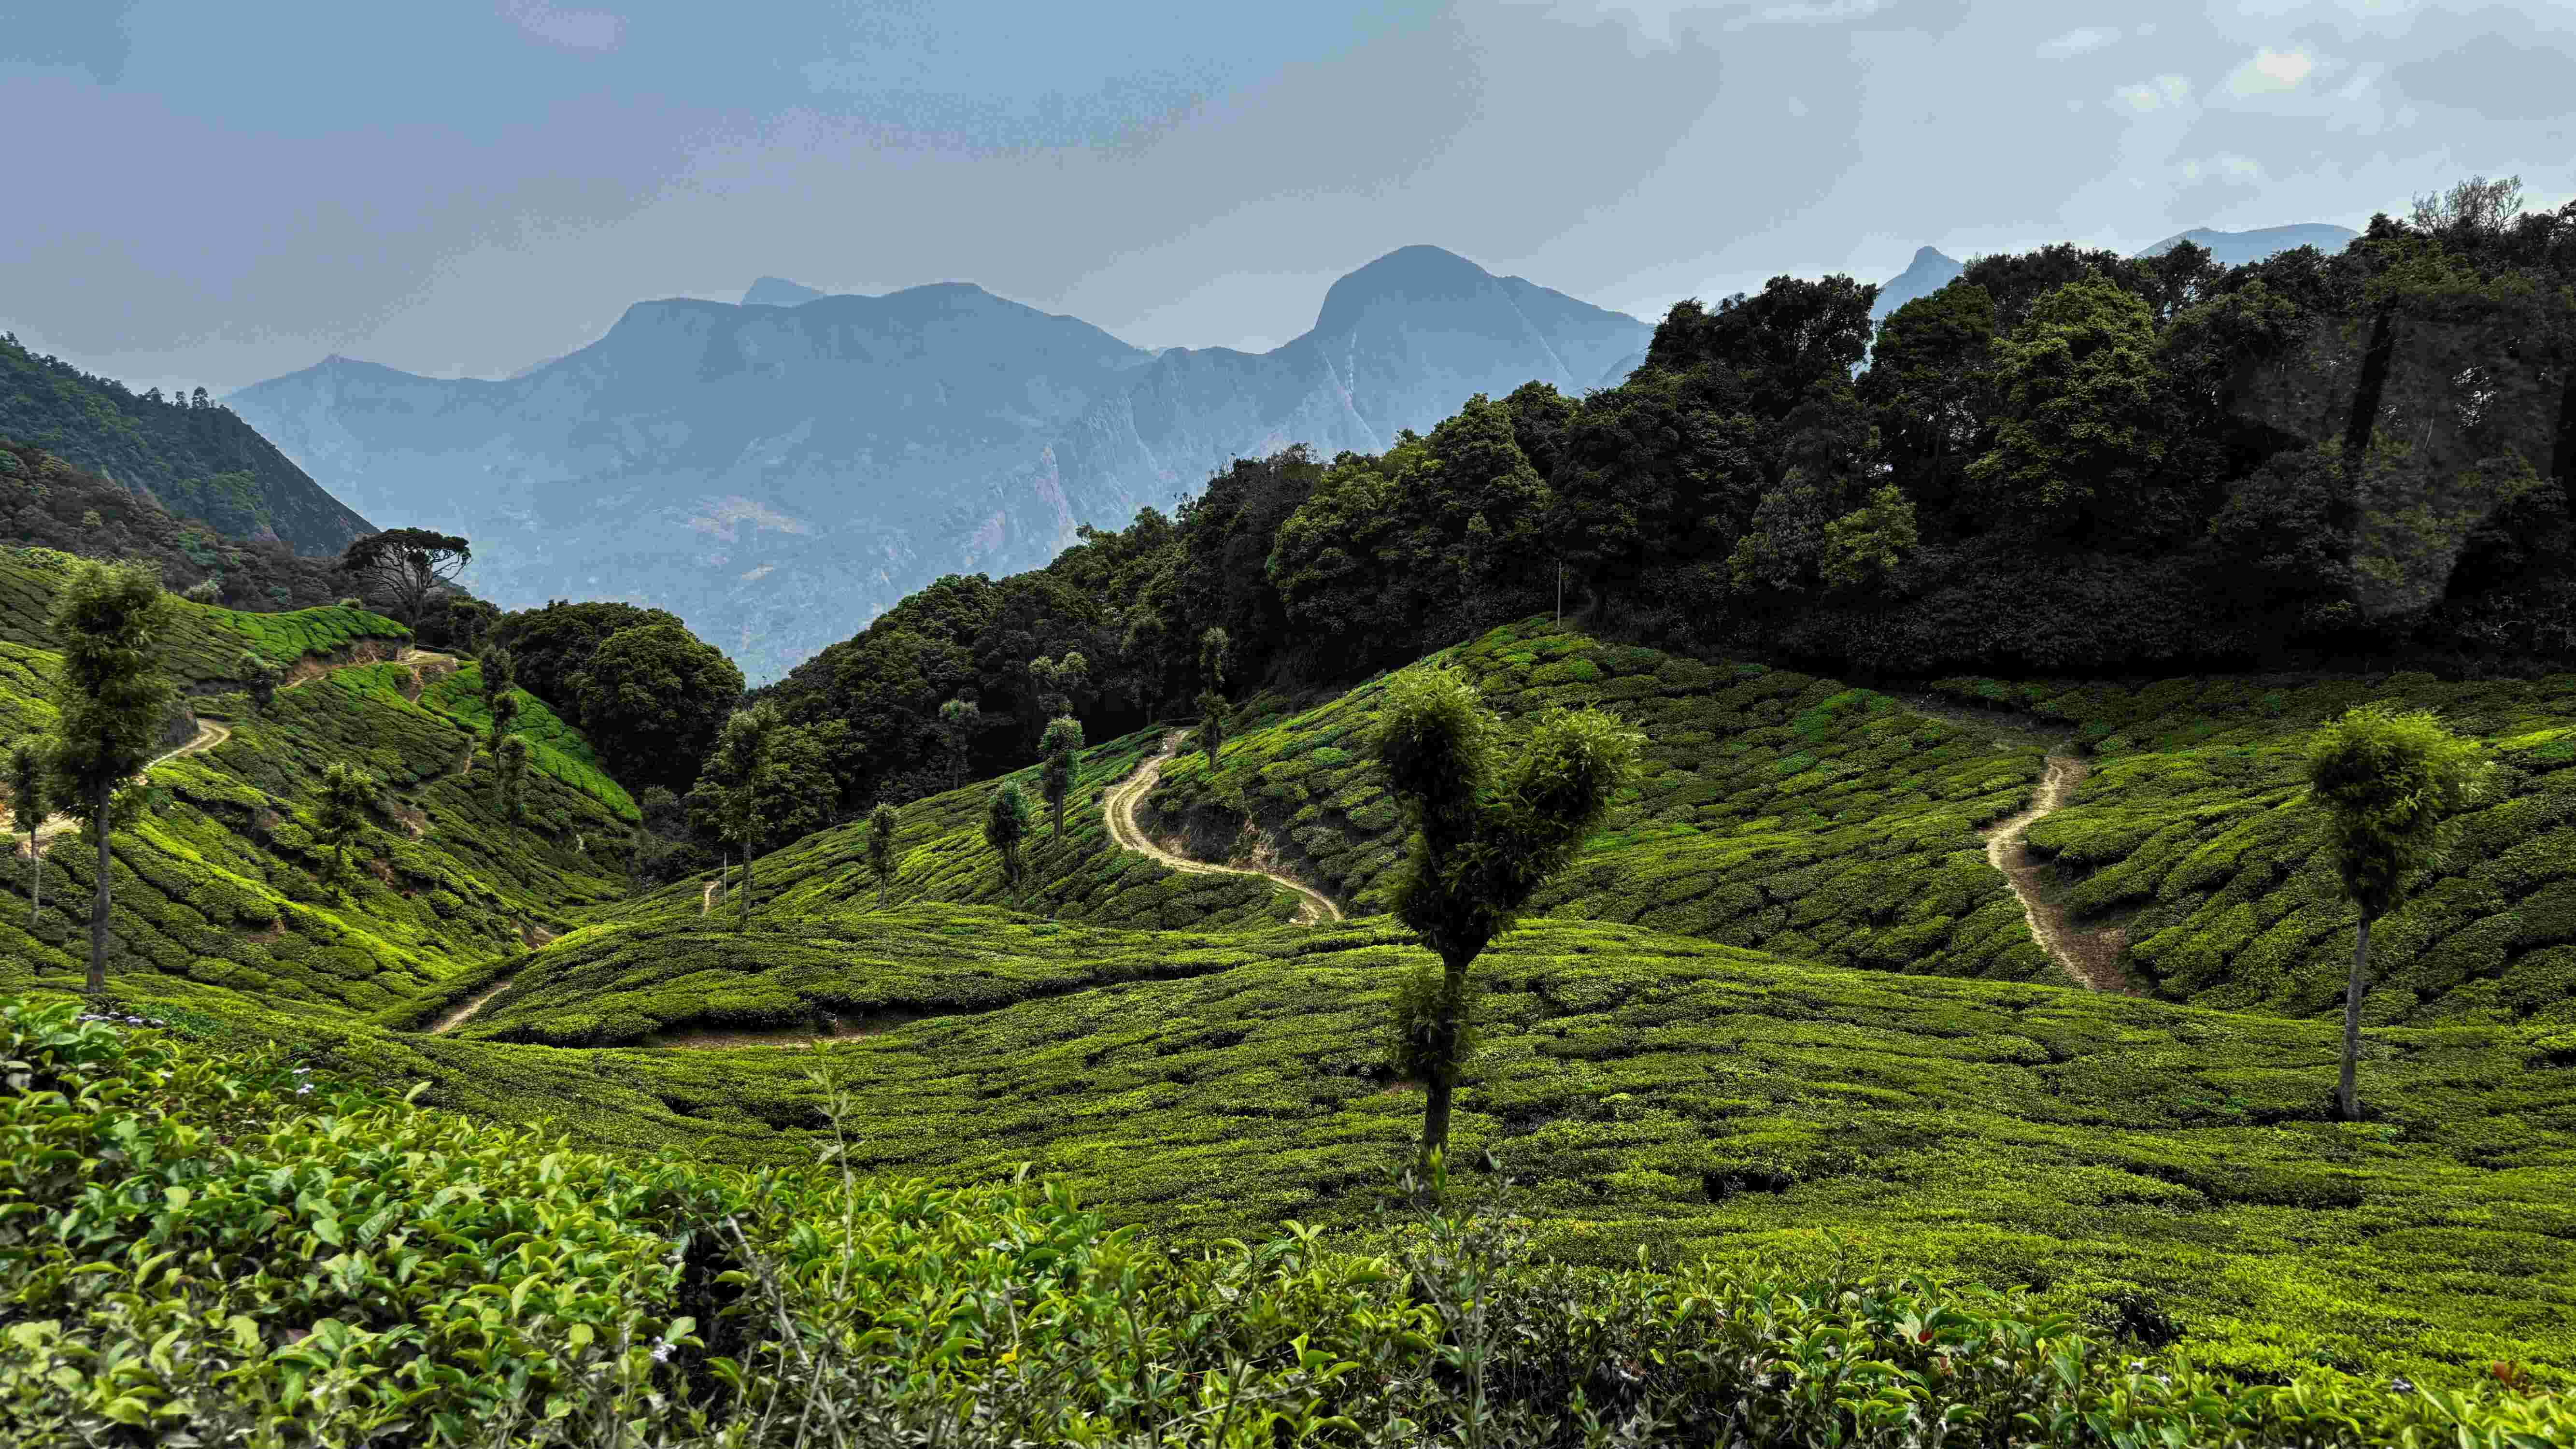
\includegraphics[width=.9\textwidth]{figs/cas-munnar-2024.jpg}
% 	\caption{The beauty of Munnar, Kerala. (See also Table \protect\ref{tbl1}).}
% 	\label{FIG:1}
% \end{figure}


% The \verb+table+ environment is handy for marking up tabular
% material. If users want to use {multirow.sty},
% {array.sty}, etc., to fine control/enhance the tables, they
% are welcome to load any package of their choice and
% {cas-sc.cls} will work in combination with all loaded
% packages.

% \begin{table}[width=.9\linewidth,cols=4,pos=h]
% \caption{This is a test caption. This is a test caption. This is a test
% caption. This is a test caption.}\label{tbl1}
% \begin{tabular*}{\tblwidth}{@{} LLLL@{} }
% \toprule
% Col 1 & Col 2 & Col 3 & Col4\\
% \midrule
% 12345 & 12345 & 123 & 12345 \\
% 12345 & 12345 & 123 & 12345 \\
% 12345 & 12345 & 123 & 12345 \\
% 12345 & 12345 & 123 & 12345 \\
% 12345 & 12345 & 123 & 12345 \\
% \bottomrule
% \end{tabular*}
% \end{table}

% \section[Theorem and ...]{Theorem and theorem like environments}

% {cas-sc.cls} provides a few shortcuts to format theorems and
% theorem-like environments with ease. In all commands the options that
% are used with the \verb+\newtheorem+ command will work exactly in the same
% manner. {cas-sc.cls} provides three commands to format theorem or
% theorem-like environments: 

% \begin{verbatim}
%  \newtheorem{theorem}{Theorem}
%  \newtheorem{lemma}[theorem]{Lemma}
%  \newdefinition{rmk}{Remark}
%  \newproof{pf}{Proof}
%  \newproof{pot}{Proof of Theorem \ref{thm2}}
% \end{verbatim}


% The \verb+\newtheorem+ command formats a
% theorem in \LaTeX's default style with italicized font, bold font
% for theorem heading and theorem number at the right hand side of the
% theorem heading.  It also optionally accepts an argument which
% will be printed as an extra heading in parentheses. 

% \begin{verbatim}
%   \begin{theorem} 
%    For system (8), consensus can be achieved with 
%    $\|T_{\omega z}$ ...
%      \begin{eqnarray}\label{10}
%      ....
%      \end{eqnarray}
%   \end{theorem}
% \end{verbatim}  

% \newtheorem{theorem}{Theorem}

% \begin{theorem}
% For system (8), consensus can be achieved with 
% $\|T_{\omega z}$ ...
% \begin{eqnarray}\label{10}
% ....
% \end{eqnarray}
% \end{theorem}

% The \verb+\newdefinition+ command is the same in
% all respects as its \verb+\newtheorem+ counterpart except that
% the font shape is roman instead of italic.  Both
% \verb+\newdefinition+ and \verb+\newtheorem+ commands
% automatically define counters for the environments defined.

% The \verb+\newproof+ command defines proof environments with
% upright font shape.  No counters are defined. 


% \section[Enumerated ...]{Enumerated and Itemized Lists}
% {cas-sc.cls} provides an extended list processing macros
% which makes the usage a bit more user friendly than the default
% \LaTeX{} list macros.   With an optional argument to the
% \verb+\begin{enumerate}+ command, you can change the list counter
% type and its attributes.

% \begin{verbatim}
%  \begin{enumerate}[1.]
%  \item The enumerate environment starts with an optional
%    argument `1.', so that the item counter will be suffixed
%    by a period.
%  \item You can use `a)' for alphabetical counter and '(i)' for
%    roman counter.
%   \begin{enumerate}[a)]
%     \item Another level of list with alphabetical counter.
%     \item One more item before we start another.
%     \item One more item before we start another.
%     \item One more item before we start another.
%     \item One more item before we start another.
% \end{verbatim}

% Further, the enhanced list environment allows one to prefix a
% string like `step' to all the item numbers.  

% %\pagebreak
% \begin{verbatim}
%  \begin{enumerate}[Step 1.]
%   \item This is the first step of the example list.
%   \item Obviously this is the second step.
%   \item The final step to wind up this example.
%  \end{enumerate}
% \end{verbatim}

% \section{Cross-references}
% In electronic publications, articles may be internally
% hyperlinked. Hyperlinks are generated from proper
% cross-references in the article.  For example, the words
% \textcolor{black!80}{Fig.~1} will never be more than simple text,
% whereas the proper cross-reference \verb+\ref{tiger}+ may be
% turned into a hyperlink to the figure itself:
% \textcolor{blue}{Fig.~1}.  In the same way,
% the words \textcolor{blue}{Ref.~[1]} will fail to turn into a
% hyperlink; the proper cross-reference is \verb+\cite{Knuth96}+.
% Cross-referencing is possible in \LaTeX{} for sections,
% subsections, formulae, figures, tables, and literature
% references.

% \section{Bibliography}

% Two bibliographic style files (\verb+*.bst+) are provided ---
% {model1-num-names.bst} and {model2-names.bst} --- the first one can be
% used for the numbered scheme. This can also be used for the numbered
% with new options of {natbib.sty}. The second one is for the author year
% scheme. When  you use model2-names.bst, the citation commands will be
% like \verb+\citep+,  \verb+\citet+, \verb+\citealt+ etc. However when
% you use model1-num-names.bst, you may use only \verb+\cite+ command.

% \verb+thebibliography+ environment.  Each reference is a
% \verb+\bibitem+ and each \verb+\bibitem+ is identified by a label,
% by which it can be cited in the text:

% \noindent In connection with cross-referencing and
% possible future hyperlinking it is not a good idea to collect
% more that one literature item in one \verb+\bibitem+.  The
% so-called Harvard or author-year style of referencing is enabled
% by the \LaTeX{} package {natbib}. With this package the
% literature can be cited as follows:


% \begin{enumerate}[\textbullet]
% \item Parenthetical: \verb+\citep{WB96}+ produces (Wettig \& Brown, 1996).
% \item Textual: \verb+\citet{ESG96}+ produces Elson et al. (1996).
% \item An affix and part of a reference:
% \verb+\citep[e.g.][Ch. 2]{Gea97}+ produces (e.g. Governato et
% al., 1997, Ch. 2).
% \end{enumerate}

% In the numbered scheme of citation, \verb+\cite{<label>}+ is used,
% since \verb+\citep+ or \verb+\citet+ has no relevance in the numbered
% scheme.  {natbib} package is loaded by {cas-sc} with
% \verb+numbers+ as default option.  You can change this to author-year
% or harvard scheme by adding option \verb+authoryear+ in the class
% loading command.  If you want to use more options of the {natbib}
% package, you can do so with the \verb+\biboptions+ command.  For
% details of various options of the {natbib} package, please take a
% look at the {natbib} documentation, which is part of any standard
% \LaTeX{} installation.

% \appendix
% \section{My Appendix}
% Appendix sections are coded under \verb+\appendix+.

% \verb+\printcredits+ command is used after appendix sections to list 
% author credit taxonomy contribution roles tagged using \verb+\credit+ 
% in frontmatter.

% \printcredits

%% Loading bibliography style file
\bibliographystyle{model1-num-names}
% \bibliographystyle{cas-model2-names}

% Loading bibliography database
\bibliography{cas-refs}


%\vskip3pt

% \bio{}
% Author biography without author photo.
% Author biography. Author biography. Author biography.
% Author biography. Author biography. Author biography.
% Author biography. Author biography. Author biography.
% Author biography. Author biography. Author biography.
% Author biography. Author biography. Author biography.
% Author biography. Author biography. Author biography.
% Author biography. Author biography. Author biography.
% Author biography. Author biography. Author biography.
% Author biography. Author biography. Author biography.
% \endbio

% \bio{figs/cas-pic1}
% Author biography with author photo.
% Author biography. Author biography. Author biography.
% Author biography. Author biography. Author biography.
% Author biography. Author biography. Author biography.
% Author biography. Author biography. Author biography.
% Author biography. Author biography. Author biography.
% Author biography. Author biography. Author biography.
% Author biography. Author biography. Author biography.
% Author biography. Author biography. Author biography.
% Author biography. Author biography. Author biography.
% \endbio

% \vskip3pc

% \bio{figs/cas-pic1}
% Author biography with author photo.
% Author biography. Author biography. Author biography.
% Author biography. Author biography. Author biography.
% Author biography. Author biography. Author biography.
% Author biography. Author biography. Author biography.
% \endbio


\end{document}